% Infrastructure section 30-01-2011


\subsection{Description}
%
% put here the description of the content of the section
%
\emph{
Responsible:  WP1 coordinator, J.v.d.Brand  \\
}
Interferometric gravitational wave detectors are large and complex and the selection of their site is an issue of great importance. The selected site should allow the highest possible level of scientific productivity at reasonable cost of construction and operation, and at minimal risk. Of paramount importance are the selection criteria that impact the scientific potential of ET. These include natural and anthropogenically generated seismicity and site geological constrains that affect critical parameters such as interferometer arm lengths. The first section of this chapter provides the requirements for the site and infrastructure of Einstein Telescope. An important aspect within these requirements is the allowed seismic motion, which is addressed according to source frequency. Seismic sources include the ambient seismic background, microseisms, meteorologically generated seismic noise, and cultural seismicity from anthropogenic activity. 

The second section describes the background on one of the fundamental infrastructure limitations called Newtonian noise. Newtonian noise originates from fluctuations in the surround geologic and atmospheric density, causing a variation in the Newtonian gravitational field. New analytical formalisms and finite element models are presented for subterranean detectors giving an estimate for NN in ET for different geologies. Using these models we show that it is in principle possible to deploy seismic sensor arrays that monitor seismic displacements and filter the detector data using Wiener or Kalman filters.

The third section discusses the ET site selection. As part of the site selection and infra-structure program for ET, 11 European sites were systemically characterised to catalogue regions within Europe that would comply with the ET site demands. Among the data that were logged were the local seismic activity, already existing local infra-structure, and population density. 

Finally, we discuss the subterranean infrastructure and cost aspects for caverns, tunnels, vacuum, and cryogenics for the ET site.
\FloatBarrier
\subsection{Executive Summary}
%
% put here a summary of the main achievement/statements of this section
%
\emph{
Responsible:  WP1 coordinator, J.v.d.Brand  \\
}
%Put here a summary of the main achievement/statements of this section \dots \par
Throughout the ET design study, the site selection and infrastructure design working group has seen an opulent evolution from a site study at 11 locations in 9 different countries, to a completely designed underground detector infrastructure. The site study has revealed several promising underground sites that comply with ET low seismic background performance requirements. In order to ascertain all site characterisation procedures were carried according to seismologic standards, measurements and data collection was carried out in collaboration with the Observatories and Research Facilities for European Seismology (ORFEUS) which is maintained by seismology department of the Dutch bureau of Meteorology. 

%At any site, seismic noise causes a secondary noise which cannot be shielded from. The local seismicity causes perturbations in the local gravity field, which are predicted by the so-called Newtonian or gravity gradient noise in gravitational wave detectors. Whereas the sensitivity of currently operating gravitational wave detectors is not limited by this noise source, second and third generation detectors will be sensitive to these gravity gradients at 10\,Hz and below. In order to predict the effect of gravity gradient noise in subterranean settings, a new analytical formalism has been developed. The analytical results were verified by finite element analysis allowing model expansion by incorporating complex geologies and inhomogeneous soils. Finally, using the analytical model and finite element results, the knowledge of the local seismicity was used to create optimal filters to remove (with certain efficiency) the gravity gradient noise from the gravitational wave detector data. 

The infrastructure definition contained several aspects such as the vacuum envelope, cryogenic infrastructure, tunnels, and caverns that are transverse through the detector optical configuration and suspension working groups. With the choice of combining a triple triangular detector with a xylophone detector topology, ET amalgamates an optimised planned disbursement for construction with a realistic proposal for a robust, highly sensitive, wide-band gravitational wave observatory. Through the design process, the vacuum system, caverns, and tunnel diameter are optimised such that the total infrastructure can be used for decades after its construction. The excavation of underground tunnels, caverns, and halls will occur over a period of approximately two years, where the ET observatory will be built in stages; the first construction stage containing a single 10\,km xylophone detector. Later the second stage will incorporate the second and third 10\,km xylophone detector.





\FloatBarrier
\subsection{The infrastructure reference design}
Einstein Telescope will have excellent sensitivity of about $10^{-22}/\sqrt{\rm Hz}$ at low frequency (2 Hz). Within the infrasound observation bandwidth, down to 2\,Hz, the scientific potential is directly affected by site location and the observatory infrastructure. Therefore, it is of paramount importance that the infrastructure reference design minimises limitations set by the selected site and the observatory infrastructure. 
\begin{figure}[h!]
	\centering
		\includegraphics[width=17cm]{./Sec_SiteInfra/Figures/ArtisticView2.jpg}
		\caption{Artistic impression of Einstein Telescope. The observatory has a triangular configuration that can house three xylophone detectors. Each detector is comprised of a low-frequency cryogenic interferometer and a high-frequency interferometer operated at room temperature. The corner stations are connected by 11 km long tunnels.}
		\label{Landscape}
\end{figure}

When choosing the observatory site and it's corresponding infrastructure, the local seismic activity is one of the most important site specific noise sources that can affect or degrade the interferometer performance. Mitigation of seismic noise is achieved by combining careful site selection, choosing a location that features low seismic noise, with advanced suspension systems (outlined in Chapter 4) providing an observation bandwidth down to 1.8 Hz. A prime example of a site that exhibits a low seismic background is the site selected for the Large Cryogenic Gravitational Telescope (LCGT) in Japan. LCGT will be located in the Kamioka mine, which currently holds the Super-Kamiokande neutrino experiment and the prototype cryogenic gravitational wave detector, CLIO. The Kamioka facility is a former zinc and gold mine and is situated 250 km west of Tokyo. Access to the underground is through a well maintained horizontal road tunnel, allowing for depths of up to 1000m. When considering that the ET performance requirements surpass those of LCGT, it becomes apparent that the infrastructure reference design advocates for a subterranean observatory and will require the realisation of substantial underground infrastructure. Section \ref{SiteInvestigation} provides an outline of the various excellent subterranean candidate sites that have been identified in Europe, which contain a similar seismic noise background to Kamioka.\\

As was explained in Chapter \ref{Ch1}, in order to construct a wide-band gravitational wave observatory, the detector topology must adopt a xylophone detection scheme containing six interferometers housed in triangular configuration. Each xylophone detector will be located in one of the corner stations and contain a high and low frequency detector pair. Fig. \ref{Landscape} shows a scaled impression of the underground observatory. The first step towards realisation of ET is the construction of the full underground infrastructure including a single xylophone detector. Fig. \ref{infra2} shows the vacuum envelope of a single xylophone detector. The bottom left corner show the vacuum towers that house the suspension systems and main optical components, which are situated in the main caverns or corner station. 

\begin{figure}[t!]
\centering
\includegraphics[width=17cm]{./Sec_SiteInfra/Figures/infra2.jpg}
\caption{Global view of a single xylophone detector showing the vacuum system and suspension towers needed to house the various optical components. Note that distances are not to scale.}
\label{infra2}
\end{figure}

The corner stations, or main caverns, in Fig \ref{Landscape} house the laser injection system and many of the interferometer seismic isolation systems that suspend the optical components. The interconnecting tunnels house the interferometer arms and have an inner diameter of 5.5 m over much of the 11 kilometres of tunnel length. Along each arm there are satellite caverns, which house the cryogenic and room temperature infrastructure for the low and high frequency input test masses respectively.  Top-level buildings, which form part of the corner stations, contain the main assembly buildings that give access to a 20 m diameter shaft and lead into the underground. In general there are two manners that can provide access to the underground; vertical access and horizontal access. Both options are discussed below and careful consideration must be taken when selecting a site that features either of these access methods.   

%Finally, the ET site studies were performed at various underground locations in hard rock (Frejus, Canfranc, Gran Sasso, Sardinia and Hungary in Europe, Homestake in the USA, and Kamioka in Japan), in salt (Slanic Salt Mine in Romenia, and Realmonte in Sicily), and in Boom clay (the HADES facility for storage of nuclear waste in Mol, Belgium). The lowest seismic noise was obtained in hardrock where it's likely to expect higher homogeneity and seismic correlation lengths. As will become evident from section 3.5, these parameters could have a significant effect on the low frequency performance of the observatory. This initial site study provide a guideline towards a medium- to long term (2 - 3 years) site study, aimed at characterising several areas within Europe that comply with long term stability of scientific driven infrastructure limitations. Examples of such limitations vary from the diurnal and seasonal local seismologic, geologic, and hydrologic conditions to the stability and support of nearby universities and government. 
\FloatBarrier
\subsubsection{Caverns}
The following section provides a general overview of the caverns, tunnels and vacuum system layout. Details about the function and/or purpose of the optical components, housed in the vacuum system, are explained in Chapter 5.

\subsubsection*{Main caverns}
Fig. \ref{infra3} shows the corner station layout with the detector vacuum envelope. Each of the corner stations has a cylindrical shape with a 65\,m diameter and contains two levels. The corner station top level has a height of 30\,m, housing the main suspension systems and vacuum envelope. The basement level contains 3.5\,m high passageways that lead to small cleanroom areas underneath the suspension systems, providing underneath access to the suspended optical components. The vacuum pipes for the low frequency (LF) and high frequency (HF) interferometer are situated on top of each other. This way, the interferometer beams propagate parallel along the vertical plane but are housed in separate vacuum pipes. For cryogenic design purposes, explained in section XX, the LF vacuum system is situated on top of the HF system.

When inspecting the detector layout in Fig \ref{infra3}, it becomes clear that each of the corner stations contain detector components from all three xylophone detectors (in Fig \ref{infra3} the detector number is denoted by the last number on the component labels). The main optical components of the interferometers need to be suspended requiring a total of 17 suspension towers in the main cavern. Four of these towers are part of the cryogenic suspension system for end test masses ETM-LF-2 and ETM-LF-3. A point of interest is that three towers contain double payloads, while another three towers contain triple payloads. Technical difficulties associated with multi-payload suspension systems are dealt with in Chapter 4. Finally, the main cavern occupies two cryolinks that protect the cryogenic end test masses ETM-LF-2 and ETM-LF-3 from thermal radiation. The cryogenic infrastructure needed for the operation of these cryolinks is discussed in section \ref{cryoinfra}.

It can be seen in Fig. \ref{infra3} that the main cavern is connected to four tunnels. Two of these tunnels accommodate six vacuum beam pipes. A third tunnel holds a single vacuum pipe while the fourth tunnel is empty. The parallel tunnel systems will be used to allow transportation of equipment between main cavern and auxilliary cavern, while also providing parallel escape routes for emergency purposes.

The laser of the low frequency interferometer, and its associated injection system, is denoted by LLF-1. The laser beam is injected into the interferometer through the power recycling mirror PRM-LF-1 and is directed towards beamsplitter BS-LF-1. Arrows indicate the directions of the two beams towards the 10 km long interferometer arms. In the same manner, the high-frequency laser, and its associated injection system, is denoted LHF-1. The high frequency laser is injected through the power recycling mirror PRM-HF-1 and propagates to beamsplitter BS-HF-1, where again arrows indicate the directions of the two beams. The HF interferometer contains two steering mirrors, both denoted SM-HF-1, after BS-HF-1 that are used to direct both beams towards the 10\,km long interferometer arms. Steering mirrors are used solely in the HF beams, since the low-frequency requirements for seismic noise isolation are less stringent for HF interferometer beams. 

After the laser beams have interacted with the interferometer test-masses, the laser beams return to the central interferometer area, where they are recombined on their respective beamsplitters. The interference signal at the beamsplitter provides the gravitational readout. A typical method called signal recycling, is employed to enhance the detected signal strength. When a gravitational wave appears in the interference signal, the signal recycling technique re-injects this signal into the interferometer to increase the interaction time with the gravitational wave itself, increasing the signal to noise ratio. The technique is explained in detail in section (5.x.x). This technique is called signal recycling and is accomplished by the mirrors SRM-LF-1 and SRM-HF-1 in the LF and HF interferometers respectively. For the LF interferometer, after the signal recycling mirror the light is bounced off three steering mirrors, indicated in Fig. \ref{infra3} by SM-SR-LF-1. These mirror steer the beam towards a set of 10\,km long filter cavities, which are used to lower the quantum noise terms entering the detection scheme (see section 5.x.x for more details on the reduction of quantum noise). 
\begin{figure}[t!]
	\centering
		\includegraphics[width=17cm]{./Sec_SiteInfra/Figures/infra3.jpg}
		\caption{Schematic outline of the main infrastructure in one of the large underground caverns. The labels are explained in the text.}
	\label{infra3}
\end{figure}

As stated above, the HF interferometer also employs the signal recycling. After the signal recycling mirror SRM-HF-1, the HF interferometer beam is injected into its own filter cavity, which lowers the laser quantum readout noise. The cavity is 700 m long and the end test mass ETM-FC-HF-1 is located in an auxilliary cavern.

As can be seen in Fig \ref{infra3}, the corner stations also house four end test masses, two from each xylophone detector. In Fig. \ref{infra3} these are indicated by ETM-LF-2, ETM-HF-2 and ETM-LF-3, ETM-HF-3 for the second and third xylophone detector pair respectively. Finally, the main cavern houses two end test masses for one of the low frequency the filter cavities. In Fig. \ref{infra3} this is indicated with ETM-FC-LF-3.



%\begin{figure}[h!]
%	\centering
%		\includegraphics[width=17cm, angle=90]{./Sec_SiteInfra/Figures/infra3.jpg}
%		\caption{Schematic outline of the main infrastructure in one of the large underground caverns. The labels are explained in the text.}
%	\label{infra3}
%\end{figure}



\FloatBarrier
\subsubsection*{Auxilliary caverns}

An impression of the infrastructure of one of the auxiliary caverns is shown in Fig. \ref{infra4}. As with the main caverns, the auxiliary caverns contain two levels with 3.5\,m high passageways underneath the 30\,m high top level. The auxiliary caverns are cylindrical in shape with a diameter of 30\,m. In its final configuration, six beam pipes pass through this cavern where the cavern is occupied by the input test masses of both the low frequency and high frequency interferometer. The low frequency ITM is a cryogenic payload and is protected from thermal radiation by cryolinks. The cavern is equipped with the necessary cryogenic infrastructure. It can be seen in Fig. \ref{infra3} that each auxilliary cavern provides the entrance to a main interferometer arm tunnel.

\begin{figure}[h!]
\centering
\includegraphics[width=16cm]{./Sec_SiteInfra/Figures/infra4.jpg}
\caption{Schematic outline of the main infrastructure in one of the auxilliary underground caverns.
The labels are explained in the text.}
\label{infra4}
\end{figure}

\FloatBarrier
\subsubsection{Tunnels}
The corner stations are connected by approximately 11 km long tunnels. These tunnels have an inner diameter of 5.5\,m and an outer diameter of 6.0\,m. At locations where cryolinks are present, the tunnel inner diameter will be increased to 6.0\,m, increasing the outer diameter to 6.5\,m. The main caverns and the auxilliary caverns are connected by parallel tunnels, running length of 700\,m. Consequently, the observatory requires more than 34 km of tunnel.
  
The tunnel system can accommodate upto six vacuum pipes. In addition, the tunnel houses the services for electricity, water, compressed air, cryogenics, safety systems and air conditioning. The diameter of the tunnel is sufficiently large to allow transportation of vacuum beam pipes. An artist impression of the main- and a single auxiliary cavern, connected by the tunnel system is shown in Fig. \ref{infra}. 
\begin{figure}[h!]
	\centering
		\includegraphics[width=17cm]{./Sec_SiteInfra/Figures/ArtisticView1.jpg}
		\caption{Artistic impression of Einstein Telescope. The observatory has a triangular configuration that can house three xylophone detectors. Each detector is comprised of a low-frequency cryogenic interferometer and a high-frequency interferometer operated at room temperature. The corner stations are connected by 11 km long tunnels.}
		\label{infra}
\end{figure}
During installation the tunnel will be equipped with a monorail system, which later is to be converted to a personnel transport system. Section \ref{assembly} discusses how the staged assembly of the observatory will work and how the monorail system is used to transport long sections of vacuum beam pipe are transported down the tunnel. During the tunnel construction, provisions are made to accommodate large vacuum valves into the tunnel walls, and to allow welding of the beam sections. For vacuum assembly and safety reasons, the tunnel is divided into 500\,m sections that are equipped with fire retarding doors, and safety shelters. Finally, the tunnel is equipped with an elaborate safety system that allows control of the airflow in order to direct smoke in case of a fire.
%\begin{figure}[htbp!]
%\centering
%\includegraphics[width=17cm]{./Sec_SiteInfra/Figures/Tunnels1.pdf}
%\caption{Schematic outline of the tunnel.
%The tunnel is occupied by the vacuum vessels that hold the low frequency (LF-1 and LF-2) and high frequency (HF-1 and HF-2) arms of two interferometers. In addition, the vacuum vessels for both filter (FC-1-1 and FC-2-1) cavities are housed. The inner diameter is 5.5 m and the tunnel wall has a thickness of 50 cm.}
%\label{fig:infra5}
%\end{figure}

\FloatBarrier
\subsubsection{Access shafts}
Presently, it is not clear whether the observatory will have horizontal or vertical access. When considering sites for ET, the manner in which access to the underground is allowed, requires careful consideration. In traditional mining, access to the underground is via a decline (ramp) or inclined vertical shaft, or adit. Shafts are considered as vertical excavations while adits are horizontal excavations into the side of a hill or mountain. 

The CMS access shaft for the LCC project at CERN, Geneva is a prime example of a large subterranean laboratory that contains a vertical access shaft. During its construction, the ground surrounding the access shaft walls were reinforced by injecting liquid nitrogen into the ground, freezing the surrounding soil. Another point to consider is that the construction of direct vertical access shafts to depths exceeding 200\,m (which might be desirable for ET) carry with it construction methods that are significantly more complex than when considering a more shallow infrastructure. All of these considerations tie in closely to the local geography and geology of a chosen site.
\begin{figure}[htbp!]
	\centering
		\includegraphics[width=17cm]{./Sec_SiteInfra/Figures/ShaftAccess.jpg}
		\caption{The construction of the CMS access shaft for the LHC project at CERN, Geneva. This shaft has an 18 m diameter and the entire CMS experiment was lowered through it. To facility its construction, the ground at the shaft walls was frozen.}
	\label{shaftaccess}
\end{figure}

Figure \ref{shaftaccess} shows an impression of the observatory with a vertical access area. Each corner station can be accessed through a 20 m diameter vertical shaft. If tunnel excavation is accomplished by tunnel boring machines, these will be lowered through these shafts. After tunnel construction, the shafts will be equipped with concrete elevator modules, staircases and will carry all services (power, water, compressed air, ventilation ducts, $etc.$). Additional shafts with a 10 m diameter are foreseen at the centre of the arms.

Finally, the top of the shafts will be integrated in large suface buildings. There the equipment of the ET interferometers, such as the vacuum system, will be prepared. Subsequently, the various modules will be lowered through the shafts into the caverns using hoisting devices.

\FloatBarrier
\subsubsection{Infrastructure safety considerations}
Safety and health will have the highest priority during every stage of the planning, design, construction, and operation of the observatory. Particular attention has to be paid key areas such as underground communication, ventilation, access, emergency egress and refuge design. During the construction of the subterranean infrastructure, the safety of both engineering and scientific personnel has to be insured. Hazards at this phase include explosions, strata collapse, vehicle collisions, fires, inundation, drowning and asphyxiation.

Ventilation and climate control within the subterranean environment is essential. In general, ventilation provides a flow of air to the underground workings of a mine of sufficient volume to dilute and remove noxious gases (typically NO$_{\rm{x}}$, SO$_2$, methane, CO$_2$ and CO). These can cause harmful physiological effects, including death. The concentration of methane and other airborne contaminants underground can generally be controlled by dilution (ventilation), capture before entering the host air stream (methane drainage), or isolation (seals and stoppings). Because gases can also poison engineers and scientists or displace the oxygen in the underground, causing asphyxiation, gas detection equipment must be installed and able to detect common gases, such as CO, O$_2$, H$_2$S. 

When working in deeper mines, high temperatures and humidity can result in heat-related illnesses, including heat stroke which can be fatal. During both construction and operation of the observatory, a ventilation system is set up to force a stream of air through the working areas. Some sources note that the operating cost for mine ventilation may account for one third of a typical underground facility electrical power budget [reference wikipedia].

Finally, after construction has finished, many of the above hazards are still risk factors and have to be addressed are. These include strata collapse, explosions, water inundation and drowning, electrocution, fire, cryogens ($e.g.$ rapid expansion > asphyxiation), and chemicals like sulphide minerals etc.   
 
%Finally, the ET site studies were performed at various underground locations in hard rock (Frejus, Canfranc, Gran Sasso, Sardinia and Hungary in Europe, Homestake in the USA, and Kamioka in Japan), in salt (Slanic Salt Mine in Romenia, and Realmonte in Sicily), and in Boom clay (the HADES facility for storage of nuclear waste in Mol, Belgium). The lowest seismic noise was obtained in hardrock where it's likely to expect higher homogeneity and seismic correlation lengths. As will become evident from section 3.5, these parameters could have a significant effect on the low frequency performance of the observatory. This initial site study provide a guideline towards a medium- to long term (2 - 3 years) site study, aimed at characterising several areas within Europe that comply with long term stability of scientific driven infrastructure limitations. Examples of such limitations vary from the diurnal and seasonal local seismologic, geologic, and hydrologic conditions to the stability and support of nearby universities and government. 

 
 
\FloatBarrier
\subsection{Site specific noise}
%\emph{Responsible:  D. S. Rabeling\\}
As was mentioned in the reference design section, it is of great importance to determine if sites contain already existing infrastructure, what the depth of the site is, and what the geologic and seismologic stability is at a given location. This last point is because site specific noise sources, like for instance seismic noise, will most likely influence the final sensitivity of the ET observatory. In order to prevent that the detector sensitivity is affected by seismically induced vibrations, current gravitational wave detectors employ seismic isolation system. Details about the proposed seismic isolation strategies for ET are explained in Chapter\,4, and for illustrative purposes, figure \ref{SuspensionArtistic} shows an artist cut-away impression of the 17\,m high suspension systems, proposed for the ET test masses. 
\begin{figure}[h!]
	\begin{center}
		 \includegraphics[width=17cm]{./Sec_SiteInfra/Figures/SuspensionArtistic2.jpg}
			\caption{Artistic cut-away impression of the ET suspension system. Such suspension chains isolate the test-masses at the bottom from seismic disturbances. For ET, seismic isolation alone will not suffice and sites with low seismic background need to be identified.}		
			\label{SuspensionArtistic}
	\end{center}
\end{figure}

%The isolation requirements for ET scale with the local seismic activity. Therefore, it is prudent to identify the areas within Europe that comply with long term stability requirements for ET and study the diurnal and seasonal variations of local seismologic, geologic, and hydrologic conditions. Section \ref{SeismicNoise} provides a background on seismic noise and its origin, for the preliminary site investigation in section \ref{SiteInvestigation}.

The seismic isolation requirements for ET scale with the local seismic activity at a given site. Thus, when scaling the seismic isolation requirements from current detectors to those for ET, it becomes clear that sites with a low seismic noise background are required to fulfil the seismic isolation target. Following in the footsteps of LCGT, site studies were therefore aimed at underground environments in Europe. The most significant results of this study are presented in \ref{SeismicResults}, showing the variation in local seismic activity in a variety geologies like hard rock (Frejus, Canfranc, Gran Sasso, Sardinia and Hungary in Europe, Homestake in the USA, and Kamioka in Japan), salt (Slanic Salt Mine in Romenia, and Realmonte in Sicily), and in Boom clay (the HADES facility for storage of nuclear waste in Mol, Belgium).  

Finally, section \ref{NewtonianNoise} provides the background on a secondary site specific noise source that originates from the local seismic activity, called gravity gradient noise. Gravity gradient noise arrises from the Newtonian coupling between the soil and the interferometer test mass. The local seismic background can be regarded as a stochastic field which causes time varying density perturbations in the soil. These density variations are the cause of a direct perturbation in the local gravity field, which of the same order (or bigger) than the gravitational wave induced signal.  

\FloatBarrier
\subsubsection{Seismic noise}
\label{SeismicNoise}
Noise studies \cite{Bard2003, Gutenberg1958, Asten1984, Peck2008} often categorise seismic noise sources according to frequency. For Einstein Telescope, critical frequency regions are in the range of 0.1 - 10\,Hz, where the seismic noise is variable mainly due to microseismic and human activity. Noise at frequencies below 1\,Hz is termed `microseismic' and its sources are dominantly natural ($i.e.$ non cultural and non-local), depending on oceanic and large-scale meteorological conditions ($e.g.$ monsoons and cyclones). Around 1\,Hz wind effects and local meteorological conditions show up, while for frequencies above 1\,Hz additional sources (besides natural) are related mainly due to human activity. Such noise is termed `cultural noise' or `anthropogenic noise'. It should be noted that the 1 Hz division is not absolute.
 \begin{figure}[h!]
	\begin{center}
		 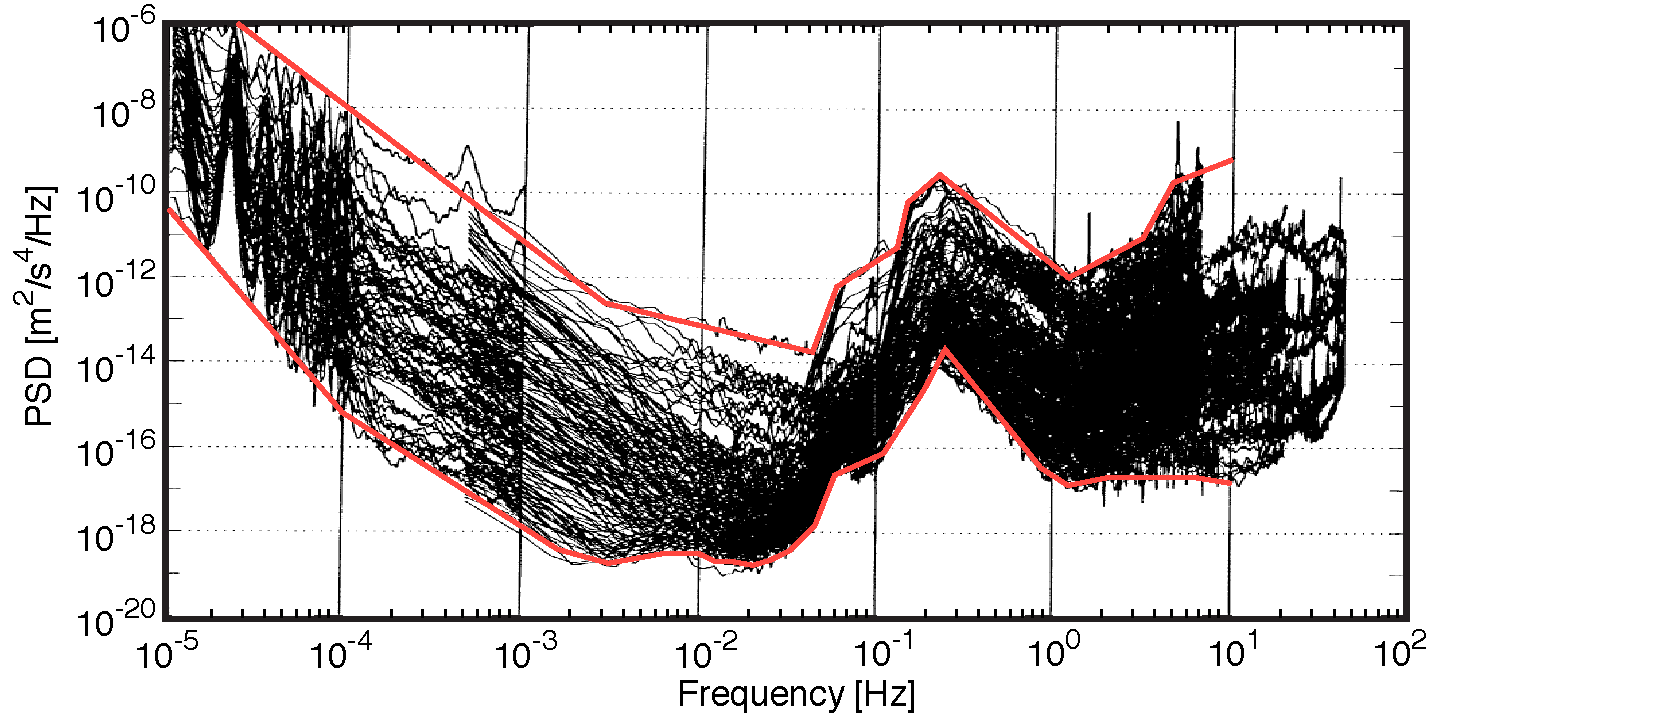
\includegraphics[width=17cm]{./Sec_SiteInfra/Figures/peterson2.pdf}
			\caption{Overlay of network station spectra used in Peterson's background noise study \cite{Peterson1993} together with straight-line segments fitted to the high-noise and low-noise envelopes of the overlay.}		
			\label{fig3.1}
	\end{center}
\end{figure}

Throughout this section seismic measurements are presented as acceleration power spectral density (PSD)\footnote{In the literature various representations are used, such as the root power spectral density (RPSD), acceleration, velocity and displacement spectral densities.} versus Fourier frequency, where PSD values have units of squared acceleration $({\rm m/s}^2)^2/{\rm Hz}$. The largest PSD values are seen at low frequencies. Here, the surface of the Earth experiences large external forces due to the gravitational attractions of the Moon and Sun. At very low frequencies this causes the surface of the Earth to rise and fall with amplitudes of about 0.5\,m with respect to the center of the Earth. This tidal motion can be seen in Fig. \ref{fig3.1} at a period of $2.3 \times 10^{-5}$\,Hz. Since the motion occurs at very low frequency the interferometer test masses will move {\sl coherently} and differential test mass motion presents no problem. Large PSD values are observed at periods clustered around $5.5 \times 10^{-2}$\,Hz and 0.2\,Hz which correspond to microseisms. Note that a large dynamic range of more than four orders of magnitude (90 dB) is needed to accommodate signals between 0.01\,Hz and 1\,Hz.

Peterson \cite{Peterson1993} catalogued acceleration noise power spectral density plots for frequencies up to 50\,Hz from 75 seismic stations distributed worldwide. Several years of data were collected (about 12,000 spectra in total). From the upper and lower bound of the combined data of both surface and borehole sensors (100 - 340\,m depth) Peterson derived, what is now known as, the new high/low noise model (NHNM/NLNM), which replaced his earlier low noise model \cite{Peterson1980}. The data including the upper and lower bound fit are shown in Fig. \ref{fig3.1}. 

As can be seen from Fig \ref{fig3.1}, microseismic ground motion is a prominent feature for frequencies around 0.07\,Hz and 0.17\,Hz. The small lower-frequency peak (periods of 10 - 16\,s) correlates with the frequency of coastal waves, where the ocean wave energy is converted into seismic energy through either vertical pressure variations or from the surf crashing onto the shore. The larger peak, at about twice the frequency (periods of 4 - 8\,s), originates from standing ocean waves that couple to the continental shelf. The standing waves are generated by superposition of ocean waves of equal period traveling in opposite directions and have recently been confirmed by satellite observations. Corresponding PSD values change up to 30 dB depending on the storm intensity, while the two frequencies shift upward as storms age.
\begin{figure}[t!]
	\begin{center}
		\includegraphics[width=15cm]{./Sec_SiteInfra/Figures/GWD_spectra3.pdf}
		\caption{Seismic acceleration PSD at current gravitational wave detector sites. The magenta dotted line represents the most critical seismic performance limits, which are set by gravity gradient noise.}
		\label{fig3.2}
	\end{center}
\end{figure}

Presently, the large interferometric detectors GEO600, LIGO, and Virgo are placed on the surface of the earth and, consequently, are sensitive to seismic disturbances. In fact, their operation is limited by seismic displacement noise and their sensitivity rapidly deteriorates for frequencies below 10 Hz. At these low frequencies Virgo has realized excellent performance due to a suitable attenuation scheme. The required seismic noise reduction for second generation GW detectors will be achieved by improving passive and active vibration isolation systems. To further suppress seismic noise in third generation detectors the test masses will be suspended from even more sizeable and complex seismic attenuators, which scheme is discussed in chapter 4. Using a simplistic model, Hild \emph{et al.} showed that by combining a scaled version of the currently used Virgo super-attenuator with data from seismic measurements at the Kamioka mine, the ET target sensitivity could be reached \cite{HildETconventional}. 

Using data from seismic measurements at the Kamioka mine in Japan Hild \emph{et al.} first showed that, using some conservative estimates for seismic isolation, the ET target sensitivity could be reached. 

Using data from seismic measurements at the Kamioka mine in Japan, and some conservative estimates for seismic isolation, Hild \emph{et al.} calculated that, in order to reach the ET target sensitivity, a requirement is set on the tolerable seismicity of a site \cite{HildETconventional}. 

For comparison, Fig. \ref{fig3.2} shows the seismic acceleration power spectral densities (PSD) of the Virgo and LIGO Hanford and Livingston sites. 

For Einstein Telescope the critical frequencies $f$ are in the range 0.1 - 10 Hz, where the seismic noise is variable mainly due to microseismic and anthropogenic activity. It is therefore important to chose a site location far from oceans and human activities (both at present and in future). The NLNM yields a PSD of $1.38 \times 10^{-17}{\rm m}^2/{\rm s}^4/{\rm Hz}$ at 1 Hz corresponding to an acceleration of $3.7 \times 10^{-9}{\rm m/s}^{2}$. Like the NLNM many remote sites show an approximately flat PSD response for accelerations in the frequency band of 1 - 10 Hz. Corresponding displacements can be found by double integration of the accelerations yielding a $1/\omega^2$ frequency dependence. The conversion should take the integration bandwidth into account (often 1/3 octave is used corresponding to a range of $\pm 10 \%$ about the center value). Note that when a Gaussian signal is passed through a narrow-band filter, the absolute peak signals of the filtered signal envelope will have a Rayleigh distribution (yielding a factor $1.253 \sigma$ for $\vert \overline{x}_P \vert$). Using the above, we find that the lowest possible displacements, according to the NLNM, are about 0.1 nm/$\sqrt{\rm Hz}$ at 1 Hz and decrease with $f^{-2}$.
\begin{figure}[t!]
	\begin{center}
		\includegraphics[width=12cm]{./Sec_SiteInfra/Figures/VirgoRoadNoise.pdf}
		\caption{Top: Seismogram recorded on the ground underneath one of the nearby bridges (top signal) and the simultaneous seismogram recorded at Virgo (bottom signal). Three heavy trucks  were crossing at approximately 5, 230, and 420s. Both signals have been bandpass filtered between 1 and 4\,Hz. Bottom: Cross-correlation of the first 100s between the two seismic channels.}
		\label{roadnoise}
	\end{center}
\end{figure}

\FloatBarrier
\subsubsection*{Anthropogenically generated seismic noise}
As was discussed above, the NLNM is a composite of different stations and instruments with different geology and in various geographic regions. Therefore, it is not possible to duplicate its response at one specific location. It has been observed that lowest noise is obtained in continental sites with sensors placed in hard rock. Sensors with low PSD values are often at borehole and subterranean stations operated at remote sites, far from cultural, oceanic, and meteorologically induced seismic noise. For ET, this means that the distance to urban areas, highways, railways, airports, etc. needs be considered. The influence of traffic induced seismicity on gravitational wave detectors have been studied by various authors. Road noise depends on road structure and materials, traffic density and vehicle type and speed. Schofield $et$ $al.$ \cite{Schofield2000} reported that local traffic, from passenger vehicles to heavy trucks, induced vibrations at the LIGO Hanford, WA, site. Vibrations were measured for frequencies in the 1 - 50 Hz range, with maxima around 4 - 12 Hz. At the Virgo gravitational wave site, road noise was analysed using recordings of the seismic field at the Virgo site and correlating these recordings with measurements underneath a major high way overpass, 3\,km away from the Virgo arms terminal building. Seismic noise originating from the nearby traffic was found in frequency ranges of 1-4\,Hz, peaking at 3\,Hz. The top plot of Fig. \ref{roadnoise} shows the seismic recordings underneath the overpass and at the Virgo end building. The bottom plot of Fig. \ref{roadnoise} shows the cross-correlation between the two signals during the first 100 seconds.  Coward $et$ $al.$ \cite{Coward2003} recorded ground vibrations at the AIGO site in Australia for vehicles passing the instrumentation as close as 24 m. Road noise was visible in the 5 - 30 Hz frequency band.
\begin{figure}[t!]
	\begin{center}
		 \includegraphics[width=14cm]{./Sec_SiteInfra/Figures/DayNightRatio.pdf}
		\caption{Midday versus midnight noise PSD ratios as a function of frequency at four different measurement sites. Cultural noise is visible for frequencies above 0.7 Hz.}
			\label{fig3.3}
	\end{center}
\end{figure}

Even in remote areas, anthropogenic noise can still be recognised. Spectrograms for frequencies up to 60 Hz have been made by Young $et$ $al.$ \cite{Young1996} with seismometers at the surface and within boreholes in the USA for data collected over more than one year. Seismometers were placed in boreholes at Amarillo, TX, at depths of 5, 100, 200, 367, 1219 and 1951 m. The anthropogenic character was present at all depths and exceeded background by about 10 dB. Its source was identified from diurnal patterns and was prominent for frequencies between 1 and 40 Hz. At Datil, NM, seismometers were installed at depths of 0, 5, 43, and 85 m and cultural noise was absent, most probably due to the remoteness of the site. At Pinedale, WY, with seismometers at depths of 3, 13, 30, 122 and 305 m, diurnal patterns in cultural noise were obscured by a pattern of progressive day-time increase of wind noise. 
\begin{table}[h] 
		\centering      % used for centering table
		\caption{Population density at the four different measurement sites. Population density figures are given in km$^{-2}$.} 
		\setlength{\tabcolsep}{10pt} 
			\begin{tabular}{l c c c}  % centered columns (4 columns) 
			\hline\hline                        %inserts double horizontal lines 
			Location & Pop. Density & Dist. to ocean/sea & Day/Night @ 10\,Hz \\  % inserts table 
			& [\,km$^{-2}$\,] & [\,km\,] & [\,dB\,] \\ [0.5ex]
			%heading 
			\hline                    % inserts single horizontal line 
			$Romania$ & 180 & 300 & 33  \\   % inserting body of the table 
			$Sardinia$ & 10 & 10 & 16 \\ 
			$Hungary$ & 75 & 500 & 9 \\        % [1ex] adds vertical space 
			$Spain$ & 1.38 & 120& 1 \\ [1ex]       % [1ex] adds vertical space 
			\hline     %inserts single line
			\end{tabular} 
		\label{PopDens}
\end{table} 

As part of the ET site characterisation, the presence and spectral PSD values of anthropogenic noise were investigated. Fig. \ref{fig3.3} shows an example of the day/night ratio obtained from four different site measurements. Respective high and low frequency disturbances can easily be recognised by comparing the listed day/night ratio values with local population density and the distance to seas and oceans, which are listed in table \ref{PopDens}. Comparing these statistics, and comparing this with the population density map of Europe in Fig. \ref{fig3.4} (data from REGIO database of EUROSTAT) corroborates the day/night ratio's found in table \ref{PopDens}. 



\begin{figure}[t!]
	\begin{center}
		 \includegraphics[width=12cm]{./Sec_SiteInfra/Figures/population.pdf}
		\caption{High frequency (1 - 10 Hz) seismic noise is driven by cultural noise. Density of population in Europe from the REGIO database of EUROSTAT \cite{eurostat}.}
	\label{fig3.4}
	\end{center}
\end{figure}

\FloatBarrier
\subsubsection*{Wind generated seismic noise}
Wind noise has been studied by a number of authors to quantify the conversion of wind energy into ground motion. The presence of wind causes movement of surface objects, such as trees or structures, or directly through turbulent pressures on topographic irregularities. Of particular interest for ET are its frequency range, the wind speed threshold for it to become evident, and its persistence with depth. 

Withers $et$ $al.$ \cite{Withers1996} performed measurements at Datil, New Mexico in the frequency band of 1-60Hz. This is a remote site that features sparse vegetation and distances to the nearest road and railroad were 12 and 90 km respectively. Measurements were performed at a depth of 0, 5, 43 and 85 m and the effect of wind noise was evident over the entire observed bandwidth with an ambient background threshold of $\sim$3 m/s. At a depth of 43m a reduction of 20 dB was found. Slightly higher reduction factors were found at 85m.
\begin{figure}[h!]
	\begin{center}
		\includegraphics[width=12cm]{./Sec_SiteInfra/Figures/wind.pdf}
		\caption{European wind resources based on data collected for the European Wind Atlas \cite{WindatlasWWW}.}
		\label{fig3.5}
	\end{center}
\end{figure}

Young $et$ $al.$ \cite{Young1996} carried out similar measurements at Amarillo, Texas at a depths of 3, 13, 30, 122 and 305 m. Wind speed thresholds, for the presence of wind induced background noise, were found to be 3-4 m/s at depths of 0-5 m and 8-9 m/s at depths below 100 m. A strong correlation between seismic noise and wind was observed over a broad frequency spectrum range from 1 to 60 Hz. The noise was 34 dB above the NLNM at a depth of 3 m, and decreased to 10 dB above NLNM at a depth of 305 m. Koller et al. (2004) determined that many parameters relating to measured ground motion caused the amplitude ratio to vary, but that only wind speed affected the frequency at which the horizontal to vertical ratio curves peaked. Mucciarelli et al. (2005) found that, provided the sensor was sheltered from direct wind (inside a concrete box at 1.5 m depth), wind increased the amplitude of all components of seismic noise (vertical, east-west, north-south) in the band 0.1-10 Hz similarly, such that ratio was unchanged. This conclusion was valid for wind speeds up to 8 m/s. 

The reductions in wind noise are a prime example that surface seismic noise contributions will decay with depth. For ET, the underground environment is expected to improve on all sources of seismic noise since surface seismic noise is exponentially reduced with depth, $e^{4d /\lambda}$, where d is the depth and $\lambda$ is the wavelength of the seismic wave. Fig. \ref{fig3.6} shows measurements at the Gy\"ongy\"osorozi mine by beker $et$. $al$. in the Hungary and indicate a factor of $\sim$10 suppression at 1\,Hz at the depth of 400\,m, and substantially more at higher frequencies. At Gy\"ongy\"osoroszi, the speed of sound at 400\,m underground (hardrock) is $\sim$3\,km/s, implying that the seismic waves in the 0.1-10\,Hz band have long wavelengths that at the surface: 300\,m - 30\,km.
\begin{figure}[h!]
	\begin{center}
		 \includegraphics[width=15cm]{./Sec_SiteInfra/Figures/Hung_transparent2.pdf}
		\caption{Measured reduction of seismic noise at the Gy\"ongy\"osorozi mine in Hungary for three different seismic sensors at depths of 0, 70, and 400m.}
		\label{fig3.6}
	\end{center}
\end{figure}

\FloatBarrier
\subsubsection{Geological and geographic considerations}

McNamara and Buland \cite{mcnamarab} have carried out a study of geographic dependence of ambient seismic noise in the USA. The strongest geographic dependence is obtained for frequencies above 1 Hz. Noise levels at the East coast are up to 50 dB above NLNM due to large population centers and represents cultural noise. Microseismism shows up in the 0.125 - 0.25 Hz frequency range (panel B) and is dominant is coastal regions. The US continental interior has noise levels about 10 dB above NLNM.

\medskip
\noindent
Recently, OneGeology \cite{onegeology}, an ambitious online project, under the direction of the British Geological Survey, started the collection of worldwide geological information. Large areas of alluvium can be identified in Europe. Allivium is deposited soft soil composed of silt, clay, sand and gravel. Its material properties vastly differ from hard rock such as granite. This has immediate consequences for the ambient seismic noise levels. The seismic data have been obtained with the ORFEUS (Observatories and Research Facilities for European Seismology) network, a non-profit foundation that aims at co-ordinating and promoting digital, broadband seismology in the European-Mediterranean area. For frequencies around 2 Hz the seismic noise is almost 40 dB higher in alluvium (stationa GE.HLG) than hardrock (station CH.GIMEL). This is caused by the lower velocity of seismic waves in sediments compared to hardrock. Areas dominated by alluvium can be found in the Netherlands, northern Germany and Poland, in the south of Germany, northern Italy (Po area), Toleda area in Spain, and eastern Europe. PSD values about 40 dB larger than hardrock have also been found in alluvium regions near Bejing, China and Santa Barbara, USA. Although for a surface site such regions should be avoided, this is not at all clear for an underground site.

\medskip
\noindent
Results of a systematic investigation of ambient noise in Germany \cite{steinwachs} were made by Steinwachs. Noise levels are lowest for sites in the south of Germany where geology is determined by kristalline granite formations. Highest ambient noise levels are recorded in the north of Germany where the hardrock layers are covered by alluvium (molasse). In between layers of harder Jura formations cover the crystalline granite. Average spectral densities are fitted with exponential functions because of strong oscillations in PSD values. The signal at 2 Hz for the smallest spectral densities has been traced by a directional analysis to Rayleigh waves originating from the coast of Norway. The signal is believed to be due to choppy water waves in the shallow North Sea hitting the shore.

\medskip
\noindent
At first sight it may be thought that Scandinavia may provide suitable sites, since it is scarcely populated leading to low cultural noise, while the surface is dominated by old, good crystalline hardrock. However, seismic measurements from the KONO station near Kongsberg, Norway, show PSD values 20 - 30 dB above the NLNM (typically 140 dB around 1 Hz). It should be noted that the KONO sensor is located in a silver mine at 340 m depth. The ambient seismic noise is due to the high frequency tail from the microseismic peak. KONO data show that the microseismic peak show large seasonal variations. Moreover, in the winter months seismic noise can be expected from ice activities in the East Sea.




\FloatBarrier
\subsection{Newtonain noise}
\emph{
Responsible:  G.\ Cella  \\
}

Another source of noise within the gravitational wave detector that originates
from the local seismic is gravity gradient noise. The seismic activity causes
perturbations in the local gravity field, which couples directly to the
interferometer test masses. Since no filter or shield can be built for
gravitational coupling, suppressing this noise source is difficult and low
seismicity sites should be identified. It is expected that an underground
environment is to improve on all associated sources of seismic noise spectral
amplitude, including seismically induced NN. Furthermore, the local
environmental conditions underground are usually stable (and controllable) and
anthropogenic-induced seismicity is much more controllable underground, where
access is limited.

The following subsections discuss this issue. 

In Subsection~\ref{subsub:NNanalyticalestimation} a simple analytical
estimations of NN is discussed. The power spectrum of NN is written as a
function of a measurable seismic quantity, under the hypothesis of homogeneity
for the medium, and neglecting any kind of effects from underground
structures.  This kind of approach is possible only with simplified models,
however it can provide guidelines expecially when detailed informations about
the geological structure of the site are not available.

A complimentary approach to analytical estimation, based on finite element
models, is presented is Subsection~\ref{subsub:NNfiniteelementmodels}. This is
the natural way to give a refined evaluation of aspects that cannot be
considered easily in the analytical approach, such as the effect of the
infrastructures and of the geological details, for example inhomogeneities.

Finally, two NN subtraction schemes are presented. In
Subsection~\ref{subsub:AmbientNNsubtraction} a subtraction scheme is presented
to monitor the NN induced by the ambient seismic background, using a seismic
sensor array. This is the approach that must be used when it is not possible
to recognize a dominant and localized source of seismic noise.

On the other hand if a strong and coherent source of noise is known (for
example a pump), a single accelerometer can be used to monitor the induced
seismic field. Using optimal filtering, the NN transfer function is estimated
from the source to the interferometer test mass, and can be subtracted from
the data. Details about this subtraction procedure are presented in
Subsection~\ref{subsub:NNsubtractionperiodic}.
\FloatBarrier
\subsubsection{A simplified NN estimate}
\label{subsub:NNanalyticalestimation}

For a given distribution of masses, which can be described by a mass density
function $\rho({\bf x},t)$, the acceleration experienced by a test mass
located at ${\bf y}$ can be written as
\begin{eqnarray}
	{\bf a}^{NN}({\bf y},t)=G\int_{V}\rho({\bf x},t)
        \frac{\bf x-y}{|{\bf x-y}|^{3}}                        
        dV_{x}
	\label{eq3.1}
\end{eqnarray}
where the integration is extended to the volume $V$ of interest.

We are interested in the fluctuating part of this quantity when the medium is
an elastic solid. From the expression of mass conservation we get
\begin{eqnarray}
	\dot{\rho}+{\bf \nabla}\cdot{\bf J}_{m}=0
	\label{eq3.3}
\end{eqnarray}
where the mass density current is given by ${\bf J}_{m}=\rho_{0}({\bf
x})\dot{\boldsymbol \xi}({\bf x},t)$, $\rho_{0}$ being the density of the
medium in the static configuration and ${\boldsymbol \xi}$ its small
displacement at a given point.

By inserting Eq.~(\ref{eq3.3}) inside Eq.~(\ref{eq3.1}) we find
\begin{eqnarray}
	{\bf a}^{NN}({\bf y},\omega)=G\int_{V}\nabla[\rho_{0}({\bf
	x}){\boldsymbol \xi}({\bf x},\omega)]
        \frac{\bf x-y}{|{\bf x-y}|^{3}}                        
        dV_{x} \label{eq3.4}
\end{eqnarray}
Note that this expression contains two different effects, as can be seen
 expanding the derivative. The terms proportional to
 $\rho_{0}{\boldsymbol \nabla} {\boldsymbol \xi}$ describe the fluctuations of
 the local density connected to the compression of the medium, while
 ${\boldsymbol \nabla}\cdot{\boldsymbol \xi} \rho_{0}$ takes in account the
 effect of the movement of density inhomogeneities, for example at the surface
 boundary.

Starting from Eq.~(\ref{eq3.4}) a general theory about the connection between
seismic measurements and NN can be developed. We will not give here the
details, which can be found for example in~\cite{Beker2010GRG}. The general
idea is to decompose seismic motion in normal modes, which are supposed to
behave as oscillators coupled to unknown stochastic forces. By measuring
quantities connected to seismic fluctuations (for example the power spectrum
of horizontal and/or vertical displacement, or the correlation between
displacements at two different points) we can get informations about the
excitation of these oscillators. Using Eq.~(\ref{eq3.4}) these can be
converted to an estimate of NN.

By making some additional assumptions a simple estimate of strain equivalent
power spectrum of NN $S_{h}^{NN}$ can be done. We will present and discuss now
this simplified result.

We model the ground as a homogeneous medium of given density $\rho_{0}$ and
the longitudinal and transverse speeds of sound $c_{L}$, and $c_{T}$
respectively. The mirrors of the interferometer are supposed to be
underground, inside a cavity whose effect can be seen to be not important in
the low frequency regime we are interested to.

As we said there will be two kind of contributions, connected to surface and
bulk fluctuations. The main assumption of the model is that the fluctuations
associated to surface Raileigh waves are dominant. In this case both the
contributions are exponentially damped with the depth, over a typical scale of
$\ell \sim v_s (2\pi f)^{-1}$ where $v_s$ is the speed of sound and $f$
the frequency.

\begin{figure}[t!]
	\begin{center} \includegraphics[width=16cm]{./Sec_SiteInfra/Figures/GeometricFactor.pdf} \caption{The
		geometrical suppression factor $\mathcal{F}$ as a function of
		the ratio between the mode's wavelength and the length L of
		the interferometer arm. $\mathcal{F}$ suppresses the NN at low
		frequencies. It is normalized to one in the high frequency
		region, where the contribution of the motion of each test mass
		is uncorrelated and adds in
		quadrature.}  \label{fig3.7} \end{center}
\end{figure}


If we assume further that damping effects are negligible, so that each mode is
excited essentially only at its natural frequency we can write now the final
expression for the NN estimate as
\begin{eqnarray}
\sqrt{\frac{S^{NN}_{h}(\omega)}{C^{seism}_{vv}(0;\omega)}}= 
\frac{4\pi G\rho_{0}}{L\omega\sqrt{2}}
\times\bigg{(}\frac{2(\beta^{2}_{T}+1)e^{\beta_{L}Kz}-(1+2\beta_{L}+\beta^{2}_{T})
e^{Kz}}{\beta_{L}(\beta^{2}_{T}-1)}\bigg{)}\mathcal{F}\bigg{(}
\frac{\omega L}{c_{T}\sqrt{x}}\bigg{)}^{1/2}
\label{eq3.36}
\end{eqnarray}
where we choose to normalize the noise to the power spectrum of vertical
surface seismic motion, $C^{seism}_{vv}(0;\omega)$.
The function
\begin{eqnarray}
\mathcal{F}(KL)=1+2J_{2}(kL)-\frac{2}{kL}J_{1}(kL)-\frac{1}{2}J_{2}(KL\sqrt{2})
\label{eq3.33}
\end{eqnarray}
which appears in Eq.~(\ref{eq3.36}) describes the coherence between the
gravitational accelerations of different test masses. It is apparently real
and it goes to zero in the low frequency regime. This is due to the fact that
when the wavelength of seismic modes is large compared with the interferometer
size each mirror feels the same acceleration, so that the length of the
resonant cavities in the arms of the interferometer does not
fluctuate. Practically it can be set to one in the frequency range of
interest.

Setting $z=0$ in Eq.~(\ref{eq3.36}) we can directly compare with previous
estimates of NN on the surface~\cite{GGSaulson, GGCellaCuoco, GGThorne},
finding essentially an agreement.

The attenuation factor, which is the ratio between the NN amplitude at a depth
$z$ and the one on the surface, can be obtained comparing the intermediate
factor between brages in Eq.~(\ref{eq3.33}). 

It is plotted in Fig.~\ref{fig3.8} (left) for several selected frequencies, as
a function of the depth.

For a given frequency NN can be zero at a peculiar depth. This in a sense is
an artifact of our oversimplified model, and depend from our assumption that a
mode contribute to the NN noise only at its resonant frequency. Another
consequence of this assumption is that the vertical seismic correlation is
proportional to $J_{0}\Big{(}\frac{\omega r}{c_{T}\sqrt{x}}\Big{)}$, so it
decrease quite slowly (as $r^{-1/2}$) at large distances, which is also quite
unrealistic.

We can take into account coherence effects by add some damping to the seismic
modes considered in the model. This is equivalent to give a finite width to
its resonant response. Just for illustrative purpose we can choose a Gaussian
line shape parameterized by a width parameter $\Gamma$ and compare the result
for the NN estimate. We do not report the analytical details here, instead we
present the result comparing the attenuation factor at different values of
$\Gamma$ in Fig.~\ref{fig3.8} (right).

We see the expected smoothing effect, and also an apparent saturation of the
attenuation factor for the smallest $Q$. This can be understood, because when
the quality factor is small there are longer wavelength modes which are
excited for a given frequency. Coherence effects have also an impact on the
estimate of NN, which will not be discussed here.
\begin{figure}[t]
\begin{center} 
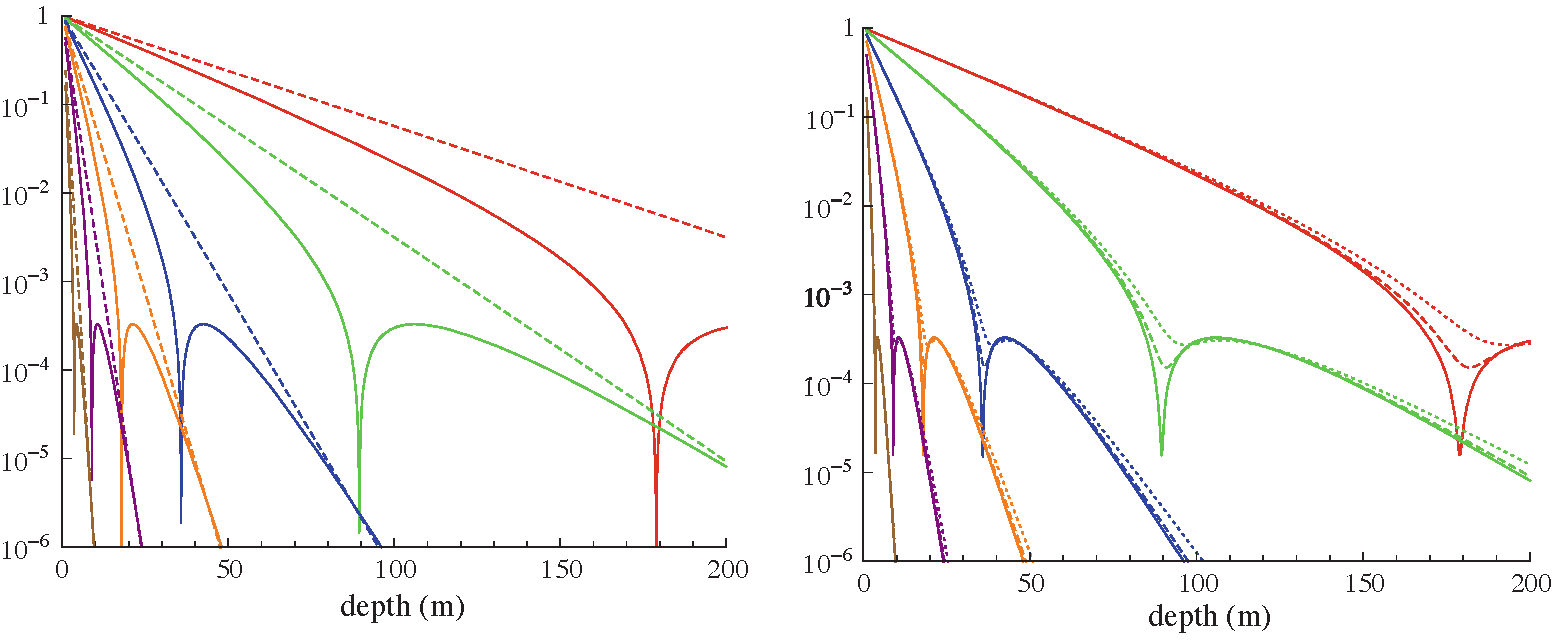
\includegraphics[width=16.5cm]{./Sec_SiteInfra/Figures/CellaNNTF.pdf} 
\caption{{\em Left}. The
		NN attenuation factor (vertical axis) predicted by
		Eq. (\ref{eq3.33}) as a function of depth (horizontal axis)
		for selected frequencies. The correspondence is red 1Hz, green
		2Hz, blue 5Hz, orange 10Hz, purple 20Hz, and brown 50Hz. Here
		$c_{T}=220m/s$ and $c_{L}=440m/s$ (continuous line) or
		$c_{L}=880m/s$ (dashed line). The zero appears when the two
		exponentially damped factors in Eq. (\ref{eq3.33})
		cancel. Before and after this point the decrease will be
		dominated by one of the two, therefore the decay constant
		changes. {\em Right}. The effect of the quality factor (vertical
		axis) as a function of depth (horizontal axis, in m) for
		selected frequencies. The quality factor is modeled using
		Eq. (\ref{eq3.36}) and corresponds roughly to $Q=10^{4}$
		(continuous line), $Q=10^{3}$ (dashed line), and
		$Q=2\times10^{3}$ (dotted line)}.  \label{fig3.8} \end{center}
\end{figure}
\FloatBarrier
\subsubsection{Finite element models}
\label{subsub:NNfiniteelementmodels}

\emph{
Responsible:  D. S. Rabeling  \\
}

Complimentary to the presented analytical descriptions of seismic activity, it will be come important, whenever considering a non-homogeneous medium or complex geologies, to have an accurate description of the seismic wave field. Simulations of such systems were accomplished using the FE software package \textit{Comsol}~\cite{comsol}. In the FE framework 3D continuum is subdivided into small hexahedral elements. Within each element the relevant physical parameters, like displacement and stress, are approximated by spline functions of arbitrary order. The following section shows how the FE software can be used to predict the NN contributions from surface and bulk waves in homogeneous media. The analysis provides the basis for simulation in non-homogeneous and/or stratified soils.

The displacement wave field that results from a seismic disturbance, is governed by the elasto-dynamic equations. The wave field in a homogeneous elastic medium can be expressed as a combination of plane body waves~\cite{seismic_schevenels}. Two types of body waves exist, pressure (P) and shear (S) waves~\cite{seismic_achenbach}. In the case of P-waves the movement of a ground particles is parallel to the direction of wave propagation. For S-waves the particle motion is perpendicular to the direction of the wave. The characteristics of seismic waves can be described by the ground properties, parametrized by  the Young's modulus, $E$,  the density, $\rho$, and  the Poisson ratio, $\nu$, describing the relationship between shear and strain forces. The wave velocities are then given by
\begin{eqnarray}
	c_P = \sqrt{\frac{E(1-\nu)}{(1-2\nu)(1+\nu)\rho}},\mbox{ and} \hspace{0.5cm} c_S = \sqrt{\frac{E}{2(1+\nu)\rho}},
	\label{eq3.38}
\end{eqnarray}
for P and S-waves respectively. Typical values for hard-rock range from 3 - 6 km/s for $c_P$, and 1.5 - 4 km/s for $c_S$.
In a medium that is bounded by another medium, such as air, or is comprised of layers, surface and head waves also exist. Head waves emerge in stratified media where modes propagating along an interface, cause energy to radiate into the low velocity zone. Surface waves are typically referred to as Rayleigh and Love waves. Love waves involve particle motion parallel to the surface and transverse to the direction of propagation. They produce no density variations and therefore have no effect on gravity gradients~\cite{GGThorne}. Rayleigh waves are polarized perpendicular to the surface and vanish with depth.

Solving the wave equation for harmonic Rayleigh waves results in the following displacement fields~\cite{seismic_rayleigh}
\begin{eqnarray}
\xi_x &=& iA(k_R e^{-\kappa_P z}-\zeta \kappa_S e^{-\kappa_S z}) e^{i(k_R x-\omega t)}, \\ \nonumber
\xi_z &=& -A (\kappa_P e^{-\kappa_P z}-\zeta k_R e^{-\kappa_S z})e^{i(k_R x-\omega t)},
\label{eq3.39} 
\end{eqnarray}
where $A$ is an arbitrary amplitude, $t$ denotes time, $\omega$ denotes the angular frequency, $z$ is the depth, $k_R$ is the wave number of the Rayleigh wave, and $\kappa_S=\sqrt{k^2_R-k^2_S}$ and $\kappa_P=\sqrt{k^2_R-k^2_P}$ are decay factors related to the shear and pressure wave numbers. Finally, $\zeta=\sqrt{\kappa_P/\kappa_S}$. The horizontal Rayleigh wave speed, $c_R$, is slightly lower than the S-wave speed and when expressed in units of $c_S$ is purely a function of $\nu$.  It can be found through $c_R/c_S = \chi$ where $\chi$ is the real root, in the range $0 < \chi < 1$ of the equation~\cite{seismic_rayleigh}
\begin{equation}
	\chi^6 -8\chi^4 + 8\left(\frac{2-\nu}{1-\nu}\right)\chi^2 - \frac{8}{1-\nu}=0.
	\label{eq3.40}
\end{equation}
The above describes harmonic Rayleigh waves propagating far from the source. In reality, excitation of a medium results in a combination of all the different wave fields; body and surface.
An important aspect for third generation GW detectors is the influence of cultural seismic noise. It has been shown \cite{WoodsASCE} that the distribution of displacement waves from an excitation with a circular footing on a homogeneous, isotropic half-space largely consists of Rayleigh surface waves: 67 \% of the energy, with 26 \% and 7 \% in shear and compression waves, respectively. One solution to reduce the cultural noise amplitude, is to move away from (sub)urban areas. Their amplitude decays exponentially and is negligible at a depth of a few Rayleigh wavelengths, $\lambda_R = 0.92 c_S/f$. Therefore, it seems natural to consider underground sites for third-generation GW detectors.
\begin{figure}[t] %  figure placement: here, top, bottom, or page
   \begin{center}
   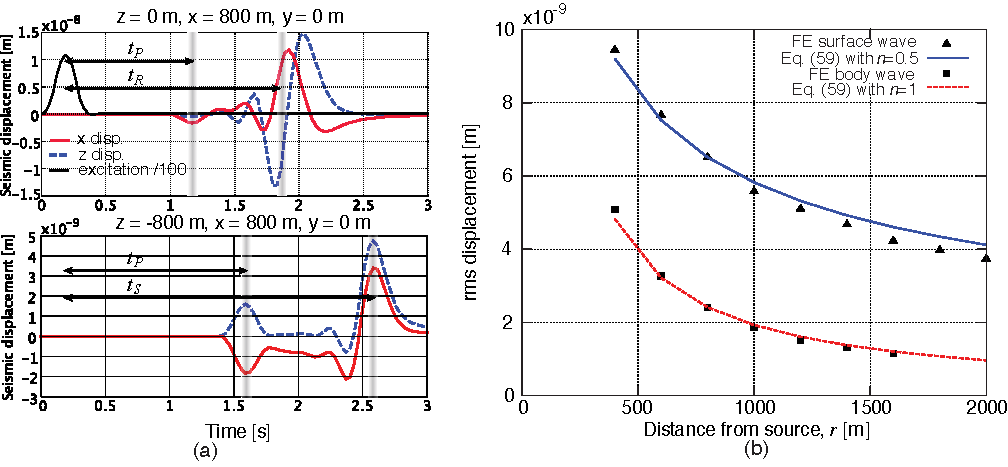
\includegraphics[width=0.9\textwidth]{./Sec_SiteInfra/Figures/Check_surfbulk.pdf} 
  \caption{(a) FE ground displacement measurements at a surface and subterranean location after a pulse excitation. P, S and Rayleigh wave arrival times are indicated. (b) The FE results for the rms amplitude of the surface and body waves with increasing distance from the source. The geometric damping contribution to Eq.~(\ref{eq3.41}) is plotted for comparison.}
 	 \label{fig3.9}
  \end{center}
\end{figure}

As waves propagate through the medium, their amplitude decreases. This attenuation can be attributed to two factors; material and geometric damping. Geometrical damping is a result of energy spreading over an increasing area. The frequency dependent material damping involves energy lost due to friction. Seismic wave attenuation for homogeneous media, can be described by~\cite{seismic_kim}
\begin{equation}
A_2 = A_1\left(\frac{r_1}{r_2}\right)^n e^{-\frac{\pi \eta f}{c}(r_2-r_1)},
\label{eq3.41}
\end{equation}
where $A_1$ and $A_2$ are the wave amplitudes at distance $r_1$ and $r_2$ from the source, $n$ is the geometric damping coefficient, $f$ is  the frequency and $c$ the propagation speed of the wave. The material damping is represented by the loss factor $\eta$. The geometric damping coefficient can be determined analytically by assessing the type of wave involved and the source type. For radial surface waves $n=1/2$ while radial body waves within the medium decay with $n=1$.

To confirm the ground motion response calculated by a FE model, the arrival times and geometric damping of the wave fields can be studied. A homogenous half-space was simulated by creating a half-sphere model with no reflection of waves incident to the spherical boundary. In view of symmetry the model could be further simplified to a quarter half-space with symmetric boundary conditions on the vertical surfaces. A single vertical excitation force was applied uniformly within a circular area at the origin with a time dependent factor given by $F(t) = A \sin^2( \pi t/T_e)$ for $0\leq t \leq T_e$ where $T_e$ is the excitation period. The amplitude scaling factor, $A$, was adjusted to create a vertical displacement at the excitation point of 1 $\mu$m.

The model has parameters $E$ = 10 GPa, $\rho=2.0$ g/cm$^3$, $\nu=$ 0.25 and a radius of 2.2 km. This results in wave speeds of $c_P = 800$ m/s, $c_S = 462$ m/s and $c_R = 420$ m/s. No material damping was implemented in this model. 

Fig.~\ref{fig3.9}a shows the FE results of seismic displacements along with expected arrival times at a location on the surface and at a depth of 800 m. Note the phase difference of $\pi/2$ between the $x$ and $z$ displacements of the Rayleigh wave. The rms wave amplitude with increasing distance from the source across the surface and within the medium are plotted in Fig.~\ref{fig3.9}b. As expected from Eq.~(\ref{eq3.41}) the wave attenuation is proportional to $1/\sqrt{r}$ along the surface and $1/r$ within the medium. 
\begin{figure}[t] 
  \begin{center}
   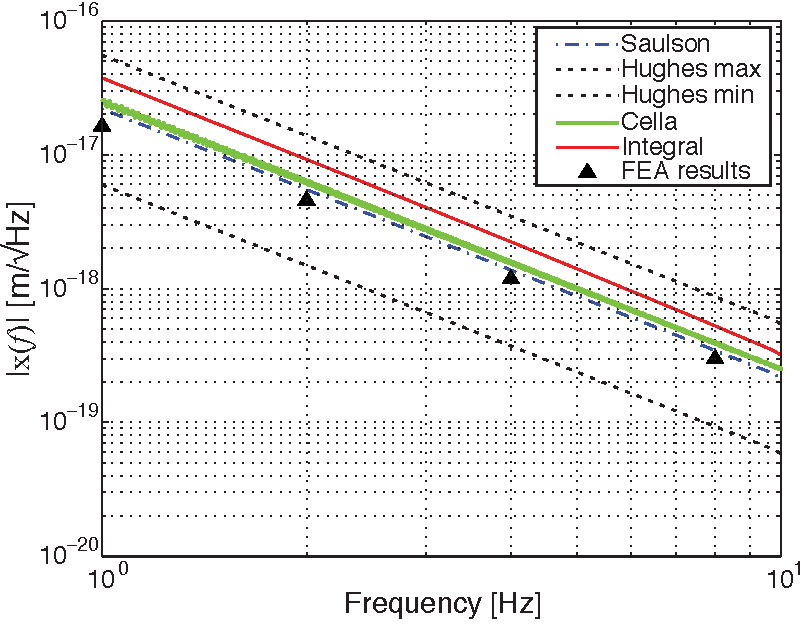
\includegraphics[width=0.49\textwidth]{./Sec_SiteInfra/Figures/ThorneSaulFEMcomparison_surface2.pdf} 
   \caption{FE calculation of the Newtonian displacement noise amplitude for a surface detector. For comparison the results of Saulson, Hughes and Thorne, and the analytic integral are shown.}
   \label{fig:FEresult}
   \end{center}
\end{figure}

With the above model, we can calculate the NN for a given distribution of masses, which can be described by the mass density function $\rho(\mathbf{r},t)$. The resulting acceleration, experienced by a test mass (i.e.\ an interferometer mirror) located at $\mathbf{y}$, can be written as
\begin{equation}
\mathbf{a}(\mathbf{y},t) = G \int_V \rho(\mathbf{r},t) \frac{\mathbf{r'}}{|\mathbf{r'}|^3}dV,
\label{eq3.42}
\end{equation}
where $\mathbf{r}$ is the position of the mass volume $dV$ and $\mathbf{r'}=\mathbf{r}-\mathbf{y}$.
In our FE analysis the acceleration is the summation of the contributions from each node $i$ with mass $m_i$ located at $\mathbf{r}_i$. The acceleration at the test mass is given by
\begin{equation}
\mathbf{a} = \sum_i \mathbf{a}_i = \sum_i  G m_i \frac{\mathbf{r'}}{|\mathbf{r'}|^3},
\label{eq3.43}
\end{equation}
with $G$ the universal gravitational constant. When a seismic disturbance is present, the nodes suffer a displacement denoted by $\mathbf{\xi}_i(\mathbf{r},t)$. The gravity gradient acceleration due to these displacements is given by
\begin{equation}
\mathbf{a}^{NN}(\mathbf{y},t) = \sum_i (\nabla\otimes\mathbf{a}_i)^T \mathbf{\xi}_i(\mathbf{r},t).
\label{eq3.44}
\end{equation}
Note that in the gravity gradient calculations presented here, the mass associated with each node is assumed to be constant. The corresponding analytical expression can be obtained by substituting $m_i \rightarrow \rho dV$ and evaluating the resulting integral.


The calculation of GGN via FE models was validated by creating simple rectangular homogenous half-space models, equivalent to those discussed by Saulson for a surface detector~\cite{GGSaulson}. The isotropic, elastic half-space with $\rho = 1.8$ g/cm$^3$, $\nu = 0.33$, $c_P = 440$ m/s and $c_S = 220$ m/s was excited on one boundary to yield plane harmonic pressure waves scaled to a flat ambient seismic noise spectrum of 1 nm/$\sqrt{\mbox{Hz}}$ between 1 and 10 Hz and the subsequent nodal displacements were recorded as a function of time. Boundary conditions were set such that no reflections occurred and seismic waves were continuous. With this input spectrum the gravity gradient displacement noise amplitude at the interferometer output was calculated and the result is shown in Fig.~\ref{fig:QS2Clay_paper}a and b. The FE results are compared with the analytic results of Saulson and Hughes and Thorne~\cite{GGSaulson}\cite{GGThorne}.
To facilitate comparison, an integral cut-off radius equal to that used in Saulson's analysis ($r_{\mbox{\scriptsize{cutoff}}} = \lambda/4$) was employed in the summation process. Fig.~\ref{fig:FEresult} shows that good agreement is obtained. To assess the effect of this cut-off the above model was calculated analytically with Eq.~(\ref{eq3.44}). Removing the cut-off leads to an increase of GGN by about a factor 2. The FE results approach those of the analytic expression in the limit that $r_{\mbox{\scriptsize{cutoff}}} $ decreases to zero.
\begin{figure}[ht]
	\begin{center}
	\includegraphics[width=0.87\textwidth]{./Sec_SiteInfra/Figures/QS2Clay_paper.pdf}
	\caption{(a) Total displacement for a time domain simulation at 2.34 seconds after a 1 $\mu$m pulse excitation at the center of the half-sphere. (b) Time domain evolution of GGN acceleration at a surface ($z$=0 m) and underground ($z$=-800 m) test mass. Only the horizontal component of the GGN acceleration is shown. Arrival times of Rayleigh, S and P-waves are also indicated.}
		\label{fig:QS2Clay_paper}
	\end{center} 
\end{figure}

The pulse excitations and the half-sphere model described earlier, were used to investigate FE gravity gradient modeling (see Fig.~\ref{fig:QS2Clay_paper}). The nodal displacements were recorded as a function of time and the GGN was calculated at various depths on a vertical line at a distance $\lambda_P= 800$ m from the $z$-axis. In order to artificially separate the contributions of the surface and body waves to the GGN acceleration the nodes with a depth less than 200 m were summed separately to those deeper that 200 m. The respective surface and body contributions were combined to give a total acceleration. Note that for times shortly after the excitation, this distinction is not precise. The results for a test mass at the surface and a test mass at a depth of $\lambda_P$ are shown in Fig.~\ref{fig:QS2Clay_paper}. Only the GGN acceleration in the horizontal direction is shown since it has the largest effect on the performance of an interferometer. The expected arrival times of the different waves are indicated in the figures and show that the Rayleigh wave dominates the GGN contribution of a detector on the surface. At a depth of $\lambda_P$ the arrival of the S and P-waves can clearly be distinguished, the S-wave producing a larger contribution, attributed to the larger seismic displacements seen in Fig.~\ref{fig3.8}a. The GGN contribution of a wave is initially negative as the wave approaches then changes sign as the wave passes by the test mass. It is interesting to note that the sign change of the surface contributions between a surface and underground detector. This is due to the sign change of the horizontal component of the Rayleigh wave for depths larger than 0.2$\lambda_R \approx 80$ m. The figure also shows that GGN builds up before any seismic disturbance actually reaches the test mass and for short times is only dependent on surface contributions.
\FloatBarrier
\subsubsection{Ambient NN subtraction}
\label{subsub:AmbientNNsubtraction}

\emph{
Responsible:  G. Cella  \\
}

A possible approach to the problem of NN mitigation is its subtraction. The basic idea is to exploit the expected correlation between NN and a set of auxiliary quantities which are continuously monitored \cite{CatichaPRE}. The natural candidates for these are seismic displacement, and we can imagine a basic scenario where a set of sensors (let's say displacement sensors) record several time series. We will consider here the simplest scenario, namely we suppose that the relevant quantities are stationary in a statistical sense. The time series recorded by the I-th sensor will be $X_I = s_I + \sigma_I$, where $s_I$ is the seismic displacement evaluated at the sensor's position and $\sigma_I$ its instrumental noise.

We will write the output of the interferometer as $Y = H + N$, where $N$ is the $NN$ and $H$ the remaining part, which we suppose uncorrelated with the seismic motion. A simple way to state the problem is asking what is the linear combination of the interferometer's and sensors' time series 
\begin{equation}
	Y_{s}=Y(\omega)+\int d\omega '\sum_{I}\alpha_{I}(\omega,\omega ')X_{i}(\omega')
	\label{eq3.45}
\end{equation}
which we can call subtracted signal which minimize the power spectrum at each frequency. The minimization variables are the functions $\alpha_{I}(\omega)$, which clearly represent linear filters that must be applied to the output of the sensors before adding them to the interferometer's data. The power spectrum $S_{Y_{s}Y_{s}}$ of the linear combination Eq.~(\ref{eq3.37}) is related to the correlation
\begin{eqnarray}
		\langle{Y_{s}(\omega)^{*}Y_{s}(\omega)}\rangle=\langle{Y(\omega)^{*}Y(\omega)}\rangle&+&\int d\omega '' \sum_{l}\alpha_{l}(\omega,\omega '')^{*}\langle{Y_{l}(\omega '')^{*}Y_{l}(\omega ')}\rangle\nonumber\\
		&+&\int d\omega ''d\omega ''' \sum_{I,J}\alpha_{I}(\omega,\omega '')^{*}\alpha_{J}(\omega ',\omega ''')\langle{Y_{I}(\omega '')^{*}Y_{J}(\omega ''')}\rangle\nonumber\\
		&+&\alpha_{l}(\omega ',\omega '')\langle{Y(\omega)^{*}Y_{l}(\omega '')}\rangle
		\label{eq3.46}
\end{eqnarray}
and minimizing this expression with respect to $\alpha_{K}(\omega ',\omega '')^{*}$ we obtain a set of linear integral equations for the optimal filters
\begin{eqnarray}
			\langle X_{K}(\omega '')^{*}Y(\omega ') \rangle+\sum_{J}\int d\omega ''\langle X_{K}(\omega '')^{*}X_{J}(\omega ''') \rangle\alpha_{J}(\omega ',\omega ''')=0
	\label{eq3.47}
\end{eqnarray}
In principle the expressoin of $\alpha_{J}$'s can be obtained by finding the inverse of the kernel $K_{KJ}(\omega,\omega')\equiv\langle X_{K}(\omega)^{*}X_{J}(\omega')\rangle$, formally
\begin{eqnarray}
		a_{I}(\omega',\omega)=-\sum_{K}\int d\omega'' K^{-1}_{IK}(\omega,\omega'')\langle X_{K}(\omega'')^{*}Y(\omega')\rangle
		\label{eq3.48}
\end{eqnarray}
If non stationary noise is present, we should define what is the relevant quantity that must be maximized, as the definition of the optimal apparatus sensitivity cannot be given it term of noise spectrum only. In the stationary case we can write
\begin{eqnarray}
		\langle X_{I}(\omega)^{*}Y(\omega')\rangle=2\pi\delta(\omega-\omega')C_{SN\,I}(\omega)
		\label{eq3.49}
\end{eqnarray}
Here the $I$, $J$ entry of the array $C_{SS}$ is the cross correlation between the seismic noise measured by the $I$th and $J$th sensors. Similar $C_{\Sigma\Sigma IJ}$ is the correlation between the intrinsic noises of the $I$th and $J$th sensors. Finally,
\begin{eqnarray}
		\langle Y(\omega)^{*}Y(\omega')\rangle=2\pi\delta(\omega-\omega')[C_{NN}(\omega)+C_{HH}(\omega)]
		\label{eq3.50}
\end{eqnarray}
is the decomposition of interferometer's power spectrum in a NN contribution plus all which is uncorrelated with it. Putting all this inside Eq.~(\ref{eq3.48}) and \ref{eq3.46} we get the optimal filters
\begin{eqnarray}
		\alpha_{I}(\omega,\omega')=-\delta(\omega-\omega')[C_{SS}(\omega)+C_{\Sigma\Sigma}(\omega)]^{-1}_{IJ}[C_{SN}(\omega)]_{J}
		\label{eq3.51}
\end{eqnarray}
which in the stationary case considered are time invariant, and the amplitude efficiency $\epsilon(\omega)$ of NN subtraction, which we define in terms of the ration between the power spectra of the subtracted $(S_{Y_{S}}(\omega))$ and un-subtracted $(S_{Y}(\omega))$ interferometer's signal spectral amplitude 
\begin{eqnarray}
		1-\epsilon(\omega)=\sqrt{\frac{S_{Y_{S}}(\omega)}{S_{Y}(\omega)}}=\sqrt{1-\frac{C^{+}_{SN}(\omega)[C_{SS}(\omega)+C_{\Sigma\Sigma(\omega)}]^{-1}C_{SN}(\omega)}{C_{nn}(\omega)}}
		\label{eq3.52}
\end{eqnarray}
Note that $(1-\epsilon)^{2}$ gives the ratio between the power spectra of the NN contained in the subtracted and un-subtracted signal. 

Equation (\ref{eq3.52}) tells us that to achieve a good subtraction efficiency three conditions are needed. First of all the sensors should be coupled as much as possible to NN, in other words $C_{SN}$ must be as large as possible. Second, the intrinsic noise of the sensor described by $C_{\Sigma\Sigma}$ should be small. Third, the correlation between quantities measured by different sensors, described by $C_{SS}$, must also be low. It is important to observe that the second term below the square root is always positive, so the procedure will never reduce the sensitivity at each frequency. 

The quantities $C_{SS}$, $C_{SN}$ and $C_{NN}$ can be estimated using a given model. $C_{NN}$ is clearly given by Eq.~(\ref{eq3.31}), and $C_{SS}$ by Eq.~(\ref{eq3.25}). A similar formula can be derived also for $C_{SN}$. Note that only $C_{SS}$ can be measured easily, so there is no real hope to fully  test the subtraction procedure without building a NN sensitive detector. 

One issue to be investigated is connected with the optimal way in which the set of sensors available must be displaced on the field. This can be studied theoretically using a given model, and optimizing Eq.~(\ref{eq3.52}) over the positions and the orientations. For illustrative purposes we report the results of a simple optimization study, done using a model with seismic correlations characterized by a single (frequency dependent) 
correlation length $\xi(\omega)$. 
\begin{figure}[t]
	\begin{center}
		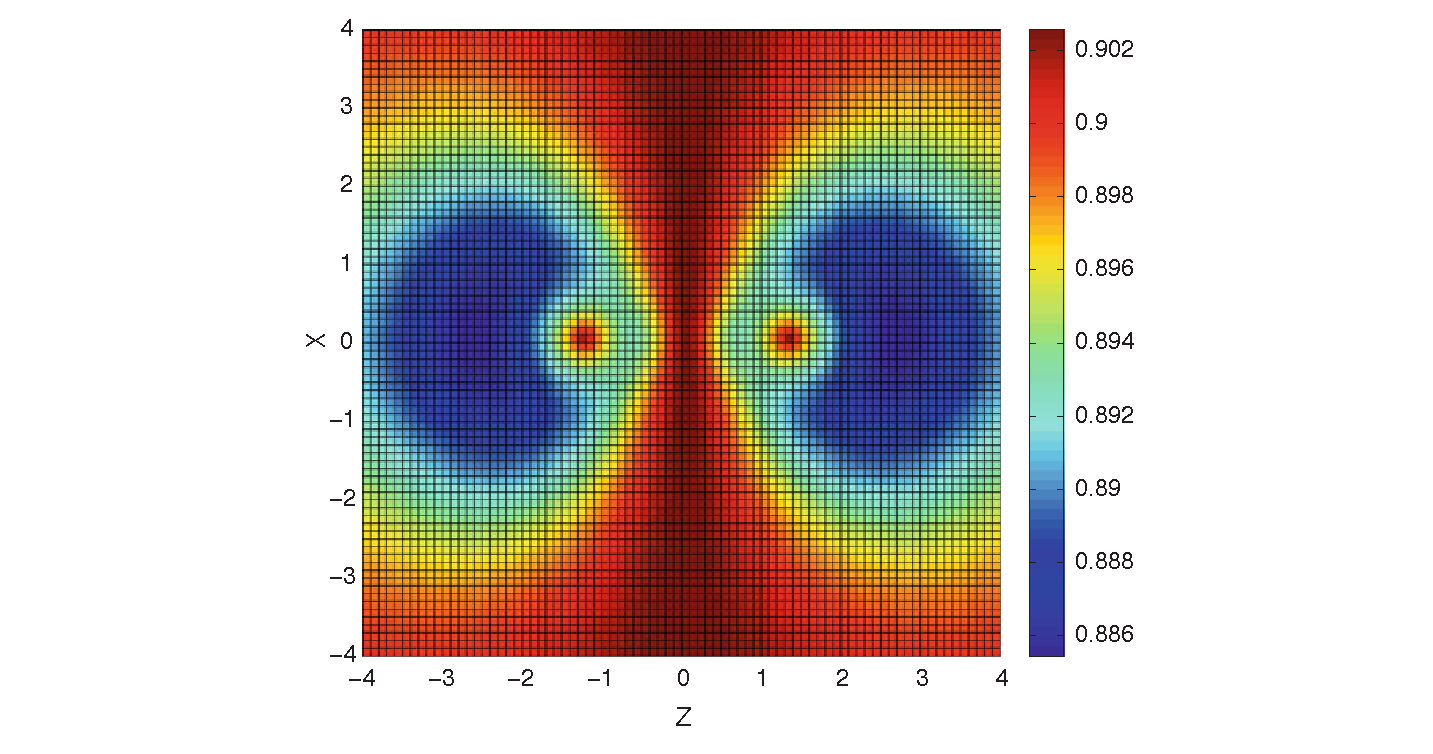
\includegraphics[width=16.5cm]{./Sec_SiteInfra/Figures/SimplOptSens.pdf}
		\end{center}
		\caption{The percentage reduction of NN on a single test mass with three sensors, for the model described by Eq.~(\ref{eq3.46}). The test mass is at the origin of the coordinate system, and the sensors measure the local density fluctuations. NN acceleration is sensed along the $z$ axis. Two sensors are fixed at their optimal positions, which are located at the circular spots at $(x,z)=(0,\pm)$. the quantity $1-\epsilon$ (see Eq.~(\ref{eq3.45})) is plotted as a function of the position of the third sensor. There is axial symmetry around the $z$ axis, so only the $x-z$ plane is displayed.}
\label{fig:NNreduction}
\end{figure}

We consider a single test mass inside an infinite medium, and we suppose that each sensor can monitor the mass density �uctuation at its position. The $i$th sensor is also affected by a intrinsic noise $\sigma_{i}(f)$, without correlations between $\tilde{\sigma}_{i}$ and $\tilde{\sigma}_{j}$ when $i\neq j$. We model the density �uctuations as a Gaussian stochastic field described by an exponential cross correlation function
\begin{eqnarray}
		\langle\tilde{\rho}(\omega,{\bf x})^{*}\tilde{\rho}(\omega',{\bf x}')^{*}\rangle=2\pi\Gamma(\omega)^{2}\delta(\omega-\omega')\exp\Big{(}-\frac{|{\bf x}-{\bf x'}|}{\xi(\omega)}\Big{)}
		\label{eq3.53}
\end{eqnarray}
The correlation functions relevant for the subtraction are easily evaluated, obtaining
\begin{eqnarray}
		C_{SS}(\omega)_{IJ}+C_{\Sigma\Sigma}(\omega)_{IJ}&=&\Gamma(\omega)^{2}\exp(-|{\bf u}_{i}-{\bf u}_{j}|)+\sigma^{2}(\omega)\delta_{IJ}\\
		C_{SN}(\omega)_{I}&=&4\pi\xi G\Gamma(\omega)^{2}\cos\theta_{I}\Psi(u_{I})\\
		C_{NN}(\omega)&=&\frac{16}{3}\pi^{2}\xi^{2}G^{2}\Gamma(\omega)^{2}
		\label{eq3.54}
\end{eqnarray}
where ${\bf u}_{I}=\xi^{-1}{\bf r}_{i}$ is the position of the $I$-th sensor measured in $\xi$ units, $\theta_{I}$ the angle between the axis along which the Newtonian acceleration is measured and the sensor's position vector and
\begin{eqnarray}
		\Phi(u)=\frac{1}{u^{2}}\Big{[}2-e^{-u}\Big{(}2+2u+u^{2}\Big{)}\Big{]}
		\label{eq3.55}
\end{eqnarray}
For a given arrangement of the sensors Eq.~(\ref{eq3.52}) becomes
\begin{eqnarray}
		1-\epsilon=\sqrt{1-3\Big{(}e^{-|{\bf u}_{I}-{\bf u}_{J}|}+\frac{\sigma^{2}}{\Gamma^{2}}\delta_{IJ}\Big{)}^{-1}\Phi(u_{I})\Phi(u_{J})\cos\theta_{I}\cos\theta_{J}}
		\label{eq3.56}
\end{eqnarray}		
With two sensors only the optimal positions are on the Newtonian acceleration axis, at a distance $d\simeq \pm 1.281 \xi$ from the est mass (we will consider only the $\sigma=0$ case). The $\cos\theta$ factor is maximized along the axis, while $\Phi(u)$ has a maximum at $u\simeq1.451$. In this optimal case $1-\epsilon\simeq0.902$. If we add a third sensor, we can evaluate $1-\sigma$ as a function of its position, which the other two fixed. This is represented in figure~\ref{fig:NNreduction}, assuming that the NN is measured along the $z$ axis. We can see how the subtraction efficiency changes with the position of the sensor, measured in unit of the correlation length. There is no improvement if we put the third sensor near the others, due to the complete correlation of the new measurement with the others. We do not gain anything from far from the test mass or at $z=0$, because in this case the measure is uncorrelated to NN. the best positions are along the $z$ axis, at a distance roughly doubled from the center. 

The model is quite crude so these are only indicative results, which however shows one expected feature. The separation between the sensors must be optimized accordingly with the typical correlation length $\xi$ of the contributions to NN we want to subtract, which depends on the frequency band where the subtraction is needed. 	
\begin{figure}[t!]
	\begin{center}
		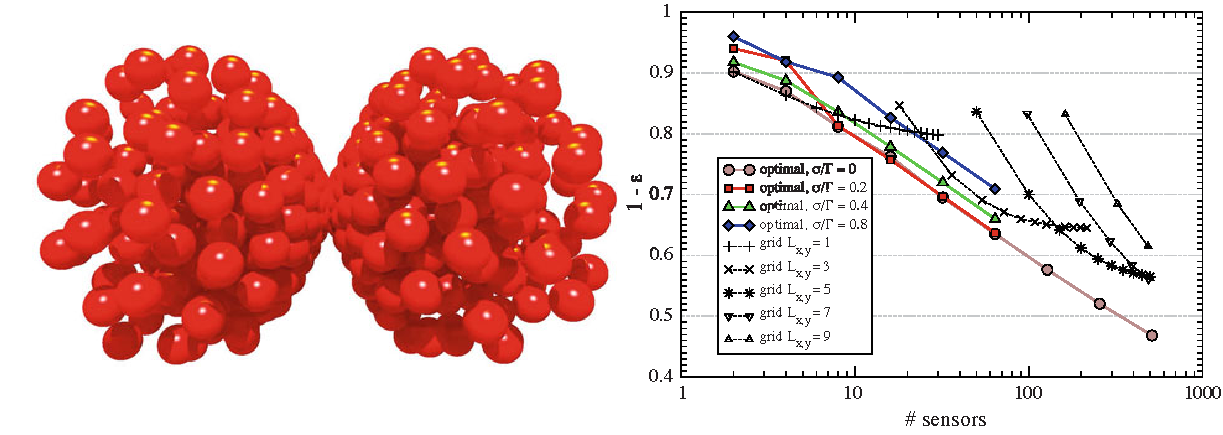
\includegraphics[width=16.5cm]{./Sec_SiteInfra/Figures/SimplOptSens2.pdf}
		\end{center}
		\caption{Left). The optimal positions for 512 sensors, evaluated accordingly with the model~(\ref{eq3.46}). Each sensor is supposed to measure the local fluctuation of density, and is represented as a sphere with the center on its position and radius $\xi$. The single test mass considered is at the center of the two clouds, and the NN is measured along the approximate axis of symmetry of the distribution. Right). The percentage of NN on a single test mass as a function of the number of auxiliary sensors, accordingly with the model~(\ref{eq3.46}). The sensors are supposed to measure the local fluctuation of density. Solid lines correspond to optimal configurations, evaluated for different intrinsic noises of the sensors. Dashed lines correspond to regular grids with sizes $L_{x}=L_{y}$ and $L_{z}$. The grid is centered on the grid and the number of sensors given by $L_{x},L_{y},L_{z}$. The NN is sensed along the $z$ axis, and $\sigma=0$ in this case.}
\label{fig:OptimalPosition}
\end{figure}

Another important point to understand is how the subtraction procedure improves with the number of sensors, and how much it is sensitive to a non optimal placement of the sensors. This is important because in a practical implementation the possibility of optimizing the placement will be limited, especially if the number of sensors will be large. It must be remembered that the optimization of the sensors' positions is a global process and all the parameters must be changed at the same time. 

Remaining in the framework of the simple model considered we optimized Eq.~(\ref{eq3.56}) for a different number of sensors. We used a simulated annealing procedure to be reasonably sure to find a global minimum. A typical result for the optimal configuration of the sensors is shown in the left illustration of Fig.~\ref{fig:OptimalPosition}. We considered 512 sensors, adjusting their positions. Each sphere in the plot has a radius length $\xi$, and is centered on a sensor�s position. We see that the spheres attempt to cover the region which is maximally coupled to NN acceleration (the test mass is between the two clouds), but they attempt also not to overlap in order to minimize the correlation between sensors. Fig. 8 correspond to the optimal configuration in the $\sigma= 0$ case. We do not show similar plots for $\sigma > 0$, however in that case we found that the overlap between the spheres increases with $\sigma/\Gamma$. This is expected because in that case a correlation between detectors can be compensated by the average of intrinsic noises. 

In the right plot of Fig.~\ref{fig:OptimalPosition} we show the relative reduction of NN as a function of the number $N$ of auxiliary sensors. The reference plot is labeled with circles, and it corresponds to the optimal configuration in the $\sigma= 0$ case. We see that the reduction of NN is quite modest, and improves slowly with N. This is partly due to the chosen model, which is quite bad from this point of view, a scan be seen with the following argument. Each sensor can be used at best to subtract the contribution to the NN of a sphere of radius $\xi$ centered on it. The number of non overlapping spheres at distance $\xi$ from the test mass scales as $n^2$, while the contribution of each of them to NN scales as $n^{-2}$. We have to sum all the contributions in quadrature, so i fall the spheres with $n<N$ are monitored we expect for large $n$ that $1-\epsilon\sim\sqrt{\sum^{\infty}_{k}k^{-2}}\sim n^{-1/2}$ or as the number of sensors $N_{s}$ scales as $n^{3}$, $1-\epsilon\sim N^{-1/6}_{s}$. 

Different models are expected to allow better subtraction performances, especially when the loss of coherence described by the scale $\xi$ is less relevant. This could be the case in some geological scenarios, while in others the simplified model presented can give an adequate description. It is an important issue, which is currently under careful investigation. 
\begin{figure}[t!]
	\begin{center}
		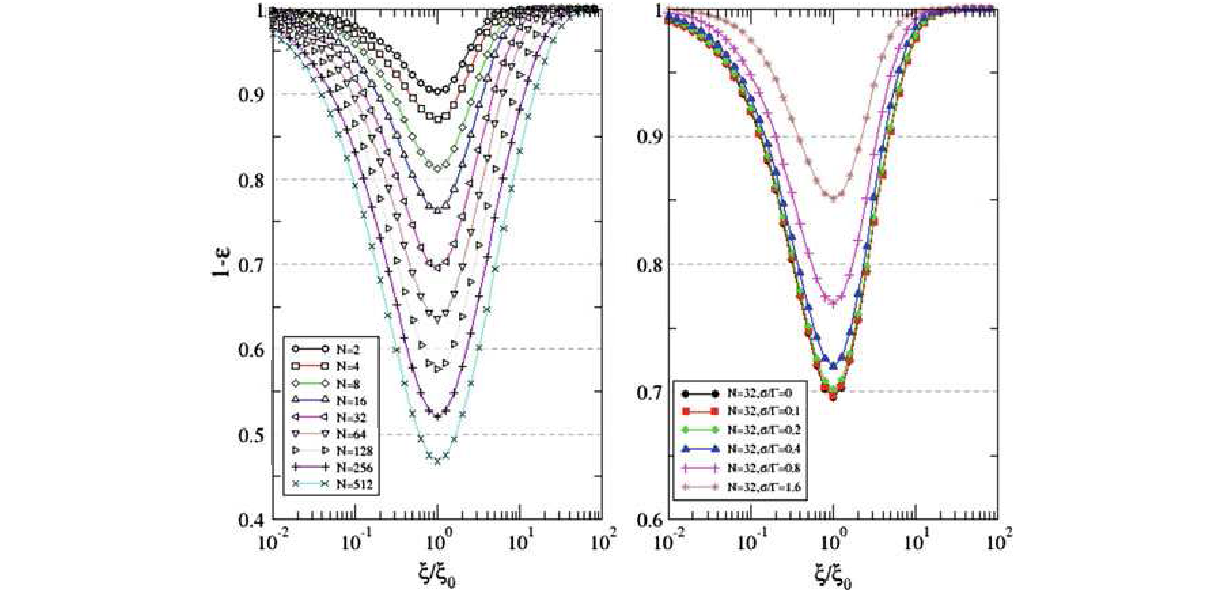
\includegraphics[width=16.5cm]{./Sec_SiteInfra/Figures/SimplOptSens3.pdf}
		\caption{On the left, the reduction of NN for a configuration of the sensors optimized for $\xi=\xi_{0}$, as a function of the ratio $\xi(\omega)/\xi_{0}$, where $\xi(\omega)$ correspond to the observed frequency. The different plots correspond to different number of sensors. On the right, for $N=$32 sensors in the configuration optimized at $\xi=\xi_{0}$, the reduction of NN is plotted as a function of $\xi(\omega)/\xi_{0}$. The different plots correspond to different values of the intrinsic noise of the sensors.}
		\label{fig:OptimalRedution}
	\end{center}
\end{figure}

Coming back to the right plot in Fig.~(\ref{fig:OptimalPosition}), the plots labeled with squares, triangles and diamonds gives $1-\epsilon$ for the optimal configuration in presence of some amount of instrumental noise. As expected there is a reduction of the subtraction performances. Finally, we showed in the same figure for comparison the results which can be obtained with a non optimal configuration, namely a regular grid of detectors with different sizes $L_x = L_x$ and $L_z$ , centered on the test mass. The optimization here is done only on the grid size, and $\sigma = 0$. The best regular grids correspond to the shapes which are best overlapped to the region coupled to NN, which means $L_{z} > 2L_{x, y}$. 

The optimization of the positions of sensors can clearly be done at a given coherence length $\xi(\omega)$, while the subtraction procedure will be applied to an entire range of frequencies (we can assume for definiteness $\xi$ proportional to the frequency). This means that the subtraction will be optimal at a chosen frequency only. 

In Fig.~\ref{fig:OptimalRedution} (left) we plotted the NN reduction as a function of the ratio $\xi(\omega)/\xi_{0}$ between the coherence length at the observed frequency and the one $\xi_{0}$ which correspond to the optimized sensors' configuration. Different plot correspond to a different number of sensors, and $\sigma=0$. A sensible reduction of the subtraction performance is evident when $\xi$ changes by one order of magnitude. This reduction is somewhat decreased by a large number of sensors. 

The effect of noise can be seen in Fig.~\ref{fig:OptimalRedution} (right). Here the number of sensors is fixed at 32, and different plots correspond to different values of $\sigma/\Gamma$. The plot suggest (with some extrapolation) that to achieve an hundred fold NN suppression, rock density (and position) fluctuations need to be measured in real time with resolution less than 1\% of the actual motion (in quiescent times in a quiet location), i.e.\ $\sigma/\Gamma < 10^{-2}$ . Because the available seismometers have been mainly developed to detect seismic events, their sensitivity is just below the normal rock activity level. A well defined subtraction pipeline has to be tested with models in order to give a precise estimate, however our conservative expectation is that seismic sensors 100 times more sensitive must be developed for NN suppression to become useful. Preliminary studies in this direction are being done at Homestake, specifically in the direction of laser strain meters and high sensitivity dilatometers. We expect that these developments, if successful, will also yield important side results in geology.
\FloatBarrier
\subsubsection{NN subtraction from periodic sources}
\label{subsub:NNsubtractionperiodic}

\emph{
Responsible:  D.\ S.\ Rabeling  \\
}
Active NN subtraction schemes have been studied both at the LIGO and Virgo laboratories [Beker, Harms, Adhikari]. Methods for active NN subtraction involve placing a witness sensor (seismometer) that monitors the noise source and estimates the noise transfer function by methods of minimising a cost function (difference between the measured noise and the estimated transfer function times the seismometer signal). The cost function that is commonly used in filter design optimisation, is the mean-square error (MSE). Minimising the MSE involves only second order statistics (correlations) and stems from the theory of linear filtering, which has many practical applications. In general, the idea is to recover a desired signal $d(n)$ given a noise observation $x(n)=d(n)+v(n)$ using some linear filter with coefficients ${\bf w}$. Minimising the cost function 
\begin{eqnarray}
		J=  E\{e^{2}(n)\} = E\{ (d(n)-\hat{d}(n))^{2}\} = E\{ (d(n)- {\bf w}^{T}{\bf x}(n))^{2}\} 
\end{eqnarray}
with the provisions that the derivative of $J$ with respect to ${\bf w}$ and the second derivative to ${\bf w}$ are zero and positive respectively, provides the Wiener, or optimal filter solution, which is useful for filter coefficients that are constant in time. If we assume that the seismic spatial distribution, generated by pumps and electricity generators, can be approximated by a Gaussian distributed impulse acting vertically onto the soil, we can use the finite element results to attempt to estimate and subtract the NN from our gravitational wave data channels. 

\begin{figure}[h!]
	\begin{center}
		\includegraphics[width=16.5cm]{./Sec_SiteInfra/Figures/nngeneration.pdf}
		\caption{Results of time domain finite element simulations for NN. Top left) Element displacement after a 1 $\mu$m pulse excitation at the center of the half-sphere. Bottom left). Element displacement at an underground location ($x$=800 m, $z$=-800 m) after pulse excitation at the center of the half-sphere. Top right). Newtonian acceleration at the surface of the half sphere due to a pulse excitation. Bottom right). Newtonian acceleration at an underground location ($x$=800 m, $z$=-800 m) due to a pulse excitation.}
		\label{fig:NNfigure1}
	\end{center}
\end{figure}


Figure~\ref{fig:NNfigure1} shows the results of a typical time domain NN simulation. The top and bottom plots on the left show the seismic excitation and the resulting displacement amplitudes at the centre of the homogeneous half space and at a depth of 800m respectively. The top and bottom plots on the right of Fig.~\ref{fig:NNfigure1} show the resulting Newtonian acceleration for a test mass placed on the surface of the half space, 800m from the excitation point and the Newtonian acceleration for a test mass placed at a distance of $\sim$1130m and 800m below the surface. Note that, in both cases, as soon as the excitation occurs a Newtonian acceleration is present at the test mass. 

The left and right plots in Fig.~\ref{fig:NNfigure1} can be interpreted as individually measured quantities, i.e.\ a NN signal in our GW detector (right) and a seismic disturbance that is measured at it's source (left). Since the disturbance is impulse like, we can estimate the NN impulse response due this disturbance from this specific source. 

Figure~\ref{fig:NNfigure2} shows the time domain estimation and subtraction results obtained using the data displayed in Fig.~\ref{fig:NNfigure1}. After the initial Wiener coefficients have been obtained, a periodic signal is placed at the center of the half sphere. Using the knowledge of the noise transfer function we can estimate the NN due to the excitation close to the seismic sensor. As can be seen, typical estimates allow subtractions of at least an order of magnitude.   
\begin{figure}[t!]
	\begin{center}
		\includegraphics[width=16.5cm]{./Sec_SiteInfra/Figures/nnsubtraction.pdf}
		\caption{Typical subtraction performance of NN using a Wiener filter. The NN originates from seismic excitations by a pump or electricity generator. NN estimates allow a subtraction of an order of magnitude }
		\label{fig:NNfigure2}
	\end{center}
\end{figure}

After ET becomes operational, it will be of great importance to minimise localised anthropogenically generated seismicity. This does not stop at restricting access to areas close to the interferometer test masses. Thorne \emph{et al.} investigated how the interferometer is affected by NN originating from humans, animals, airplanes, etc.~\cite{GGthorneWinstein}. Within the subterranean environment this extends to placement of electricity generators, pumps, and cryo-coolers to keep the facility operational. These devices will be sources of seismic noise and will therefore generate continuous NN. 
\FloatBarrier
\subsection{Site selection}
\emph{
Responsible:  D.\ S.\ Rabeling  \\
}

As described in the previous sections, ground motion may prove a limiting factor for the low frequency performance of ET. A preliminary site investigation was carried out to make a comparative analysis of various (underground) locations throughout Europe and across the globe. The following paragraphs will discuss the measurement procedures and a list of locations that have undergone investigation. In order to ascertain all site characterisation procedures were carried according to seismologic standards, measurements and data collection was carried out in collaboration with the Observatories and Research Facilities for European Seismology (ORFEUS) which is maintained by seismology department of the Dutch bureau of Meteorology. This will include a summary of the results from each location as well as the data collected at these sites. 
%the data from a large number of seismic stations in Europe is available to us through the Orfeus network.	 
\FloatBarrier
\subsubsection{Measurement methodology and data analysis}
\emph{
Responsible:  D. S. Rabeling  \\
}
In order to measure the ambient seismic background requires low noise broadband seismometers. All seismic measurements were carried out using two measurement stations, each station consists of a Trillium 240 (T240) accelerometer and a data acquisition system. The T240 is a broadband low noise seismometer with a flat velocity response from 4 mHz to 35 Hz and a self noise below the Low noise model  from 0.01 to 10 Hz. The seismometer is placed on top of a granite tile that is fixed to the solid rock floor with tile glue. A thermal and acoustic insulation cover is then placed over the seismometer. The read-out of the seismometers is done using a portable data acquisition system consisting of a 19 inch rack mounted computer with a national instruments 18 bit DAQ card, a low noise amplifier, a battery UPS and a power supply to both the seismometer and amplifier. 

The seismometer produces a sensitive measurement of the ground velocity in 3 directions (north, east and vertical) and a number of diagnostic signals. The velocity channels are amplified by a factor of 105 to increase the resolution of the read-out system and passed through a low-pass filter with a -3 dB point at 30 Hz. The sampling rate is 128 Hz and every 128 seconds of data are written away into a single ascii data file using a LabView program. 

The noise budget for each seismic measurement station has two major contributors; the self-noise of the T240 and the amplifier and ADC noise. The ADC noise in terms of an acceleration PSD, denoted by $PSD_{noise}(f)$, can be modeled using the following equation [Sleeman].
\begin{equation}
\mbox{PSD}_{\mbox{noise}}(f) = \left(\frac{2A}{2^n}\right)^2 \cdot \frac{1}{12 \cdot f_{N}},
\label{eq:PSDnoise}
\end{equation}
where $A$ is the full-scale amplitude to the input of the ADC, $f_N$ if the Nyquist frequency (related to the sampling frequency, $f_N = f_s/2$) and $n$ the number of quantization levels (or bits). Fig.~\ref{Fig:Seis_noise} shows the outcome of Eq.~(\ref{eq:PSDnoise}) with the seismic stations DAQ parameters ($n=16$, $A=10$ and $f_{N}=64$), along with the T240 self-noise provided by the manufacturer and the measured DAQ and amplifier noise. The latter was obtained by short-circuiting the amplifier input with a impedance equal to the of the seismometer output ($300\Omega$). The DAQ and amplifier noise is consistent with the expected values from Eq.~(\ref{eq:PSDnoise}), the dip in measured noise above 10 Hz is due to the seismometer response function. This suggests that this noise source is limited by the ADC noise. The total noise of the system stays below the NLNM between 0.03 and 8 Hz and is dominated by the T240 self-noise, except between 0.3 and 20 Hz.
\begin{figure}[h]
	\begin{center}
		\includegraphics[width=0.65\textwidth]{./Sec_SiteInfra/Figures/compare_noise}\hspace{1pc}%
		\caption{Noise characterization of the seismic data acquisition system. The theoretical DAQ limit is calculated from Eq.~\ref{eq:PSDnoise} and the Trillium 240 self-noise as provided by the manufacturer. The total noise is below the low noise model between 0.03 and 8 Hz.}
		\label{Fig:Seis_noise}
	\end{center}
\end{figure}

On site measurements are made over a period of 5 to 6 days. Care is taken to ensure that the measurement time includes at least a weekend and a number of week days. To characterize seismic measurements the amplitude of each frequency component of the velocity channels are calculated using Fourier analysis. In all of the following results a fast Fourier transform (FFT) was performed on stretches of 128 seconds of data to obtain a acceleration PSDs in units of (m$^2$/s$^4$)/Hz. The PSDs are averaged over a period of half an hour. Averaged PSD values are smoothed by taking the average of the PSD values in a constant relative bandwidth of 1/10 decade. (So for low frequencies the averaging is over only a few points, for high frequencies the averaging is over much more points). A means of comparison is required to give an impression of the relative amplitude of the seismic noise. To do this the new high and low noise models are used. These models indicate theoretical values for extremely high and extremely low seismic noise locations respectively. Spectral variation plots are used here to not only show the amplitude of the seismic signal but also how much time, as a percentage, is spent at a certain level. This is indicated by the color of the plot. The spectral variation plots also contain three solid line plots to indicate the mode and the 90 and 10\% levels. The mode is the most common PSD value in each frequency bin, and 90 and 10 \% levels indicate the point under which the PSD will stay for 90\%, 10\% of the time respectively. 
\FloatBarrier
\FloatBarrier
\subsubsection{Measurement sites}
\emph{
Responsible:  D. S. Rabeling  \\
}

The following section provides a brief description of all locations included within the site characterisation and classification program. The locations that were incorporated are displayed on the map of Fig.~\ref{Fig:map}. The selection criteria for these sites was based on the availability of a suitable underground measuring location. Gaining safe access to underground locations with little or no nearby (underground) activity proved very challenging. The majority of the sites are therefor already existing underground laboratories or decommissioned mines that are undergoing environmental rehabilitation or being converted for tourist purposes. Initial selection procedures were based on general suitability for an ET detector and surface measurement of seismic data. The main purpose of this research was to ear-mark 3 or 4 locations for an extensive seismic and geological study. A followup site selection study would address in more detail the suitability of constructing an ET at or near the location or in similar geological conditions.  


\begin{figure}[h]
	\begin{center}
		\includegraphics[width=0.65\textwidth]{./Sec_SiteInfra/Figures/map}\hspace{1pc}%
		\caption{Map displaying  the European locations presented in this report. Red icons with a dot indicate locations where measurements where taken at underground locations, blue icons indicate where data was obtained via the Orfeus network from surface installations.}
		\label{Fig:map}
	\end{center}
\end{figure}

\begin{itemize}
\item \emph{Italy: Gran Sasso.}
The Gran Sasso National Laboratory is the largest underground combined laboratory in the world for experiments in particle physics, particle astrophysics and nuclear astrophysics. It is located between the towns of L'Aquila and Teramo, about 120 km from Rome. The underground facilities are located on one side of the ten kilometer long freeway tunnel through the Gran Sasso Mountain at an average depth of 1400 m. They consist of three large experimental halls, each about 100 m long, 20 m wide and 18 m high and service tunnels, for a total volume of about 180,000 cubic meters.

\item \emph{Italy: Sardinia.}
The island of Sardinia is centrally positioned with respect to the European tectonic plate, which results in a seismically much quieter more stable domain than the Italian main land. Measurements were performed in a mine near Lula, 50 km south of Olbia on the north-eastern side of the Island. This former lead-zinc mine is currently being rehabilitated to allow safe passage into the mine for tourists. 

\item \emph{Italy: Sicilie.}
The Italkali salt mine is an active mine situated near the town of Realmonte on the southern coast of Sicily, 10 km east of Agrigento. Salt is excavated by creating large caverns, some exceeding dimensions of 100 m in length and 35m in height. Measurements were taken at a depth of 60 m below the surface, at an elevation of 30 below sea level. Both stations were installed in a storage cavern about 50 meters apart. One seismic station was on a large concrete pad with the other was placed straight onto the salt floor.  

\item \emph{The Netherlands: Heimansgroeve.}
The Heimansgroeve is an old quarry situated at the southern tip of the Netherlands. It contains the oldest rock sort found in the Netherlands, Carboniferious, about 360 - 300 million years old. The stone consists of slate and carbonic sandstone and holds a seismic observatory maintained by The Royal Netherlands Meteorological Institute, some 10 meters below the surface.

\item \emph{Hungary: Gy\"ongy\"osoroszi.}
The Gy\"ongy\"osoroszi mine is situated some 107 km North-East from Budapest in the M\'atra mountains. This old zinc-lead mine has horizontal access with underground depths ranging from 100 to 350 m at an elevation of $\sim$400 m. Local rock type consists of andezit and andezit tufa. A ecological rehabilitation of the neighborhood and mine was started last year. The mine contains a number of long straight drifts of which the longest is 3 km. There is a permanent Seismological Observatory of the Hungarian Academy of Sciences at Piszk\'estet\"o on the site of the Konkoly Thege Astronomical Observatory. It is situated about 4 km from the mine entrance.

\item \emph{Romania: Slanic.}
Slanic-Prahova is located, 40 km NE of Ploiesti, or 100 km north of Bucarest in Romania. The salt layers in the area allow large caverns (30m wide and 35m high) to be dug. The salt exploitation ended in 1971, however another salt mine is still active in the same salt deposit. For the time being the mine contains a low background laboratory in one of the caverns. Access into the mine is via an elevator, able to carry up to 10 tons. The current network of galleries of Unirea salt mine are very large, extending an area of 70 000 m2 with 2.9 million m3 having already been excavated. 

\item \emph{France: Frejus.}
The underground laboratory LSM ``Laboratoire Souterrain de Modane'', is located along the road tunnel between the Frence Modane and Italy. The overburden at this site is 1700 m of hard-rock or 4800 meters of water equivalent. The LSM, in operation since 1982, already hosts two particle physics experiments requiring an extremely low-background environment to study neutrino properties and to search for Dark Matter.

\item \emph{Spain: Canfranc.}
The Canfranc Underground Laboratory (LSC, ``Laboratorio Subterr\'aneo de Canfranc'') is located on the Spanish side of the Pyrenees, under the mountain of ``El Tobazo'' and has various particle physics programs aimed at very low background experiments for the study of neutrino properties and the search for Dark Matter. It has 2500 m water equivalent overburden at depths of around 900 m and can be accessed via the roadway or decommissioned railway tunnels.

\item \emph{Germany: Black Forest.}
The Black forest observatory is a geophysical observatory in operation since 1972, owned and operated by Karlsruhe University and Stuttgart University. It is located in an abandoned silver mine and contains gravimeter, seismometers, tilt-meters as well as electromagnetic and weather sensors. The local rock type is granite and the overburden is up to 180 m.

\item \emph{Finland: Sumiainen.}
The Finish bedrock is amongst the oldest and most stable in Europe, ranging from 3.5 to 2.6 billion years old, making it cheap and relatively trivial to construct underground caverns and tunnels. For this reason much of the infrastructure in Finish cities is built underground. Finland's isolation from major oceans and small population density could prove ideal for a low seismic background environment. No site was visited but data from an already installed surface seismic observatory in central Finland, near Sumiainen, was acquired.

\item \emph{Belgium: Mol}
Near Mol in northern Belgium an underground laboratory has been constructed to investigate the long-term effects of construction in the "Boomse" clay layer. Clay is impenetrable to water and has self healing properties. For these reasons it has been proposed as an excellent candidate for the long-term storage of highly active nuclear waste. The HADES underground laboratory administered by EURIDICE is situated at a depth of 230 m in a clay layer roughly 150 m thick. In 2002 a new gallery was constructed, in a cylindrical form with a diameter of 4 m and a length of 80 m. A seismic station was setup in the new gallery and measurements were taken during the Christmas break of 2010.


\end{itemize}
\begin{figure}[t!]
	\begin{center}
		\includegraphics[width=0.9\textwidth]{./Sec_SiteInfra/Figures/sosanattos2}
		\caption{Underground map of the Sos Enattos mine, Sardinia. The yellow spot indicates the measurement location, at an elevation of 206 m and depth of 189 m.}
		\label{fig:sosanattos}
	\end{center}
\end{figure}

%%%%%%%%%%%%%%%%%%%%%%%%%%%%%
%		 sites
%%%%%%%%%%%%%%%%%%%%%%%%%%%%%
\FloatBarrier
\subsubsection{Results from a selection of sites}
\emph{
Responsible:  D. S. Rabeling  \\
}

The following section discusses, in more detail, three sites that have been selected for further investigation. Seismic measurement results will be presented and discussed, then summarized in the following section. 
\FloatBarrier
\subsubsection*{Sos Enattos mine, Sardinia, Italy}
The Sos Enattos mine, Lula, Sardinia, is a former lead and zinc mine of schist rocks composed of sphalerite ([Zn,Fe]S) and galena (PbS). It is situated 50 km south of Olbia on the north-western side of the island, 20 m from the coast. A map of the mine is shown in Fig.~\ref{fig:sosanattos}. The experimental areas where the seismometer stations were placed was at a depth of 189 m, at an elevation of 206 m above sea level, which are indicated by the yellow circles in Fig.~\ref{fig:sosanattos}. Data was collected during the period of June 31, to July 5, where the most significant results, obtained by applying the analysis method described in a previous section, are presented below.

The spectral variation plots, data taken from the Sos Anattos mine, are shown in Fig.~\ref{fig:Lula-A_multiplot1}. The primary and secondary microseismic peaks are visible at 0.08 and 0.2 Hz respectively and are within an order of magnitude or touching the low noise model. This is due to the relatively large distance to the atlantic ocean (1000 km to west coast of France). At higher frequencies, between 0.4 and 0.8 Hz an extra "tertiary" microseismic peak can be seen. This is due to similar effects that cause the primary and secondary micro-seismics, but its origin stems from the Mediterranean sea and are typical of other Italian sites~\cite{marchetti}.
\begin{figure}[h!]
	\begin{center}
		\includegraphics[width= 0.8\textwidth]{./Sec_SiteInfra/Figures/Lula-A_multiplot1}
		\caption{The horizontal (left) and the vertical seismometers component (right) power spectral densities, plotted as a spectral variation from the Italy - Sardinia site. The "tertiary" microseismic peak as a result of microseismics from the Mediterranean sea is evident from 0.4 to 0.8 Hz. Large variations at higher frequency are a results of work in the mine and anthropogenic activity.}
		\label{fig:Lula-A_multiplot1}
	\end{center}
\end{figure}

When inspecting the spectrograms in Fig.~\ref{fig:Lula-A_multiplot2}, it becomes clear that, in the frequency range from 2 to 20 Hz, there is a relatively large variation in the spectral density. It is easy to see that PSD variations at these frequencies occur according to a daily pattern, indicating that sources of seismic noise at these frequencies are from anthropogenic nature. More over, in the 2 - 8 Hz range the heightened activity seems to occur during the late morning hours before noon, on all days except sunday. This coincides with the miners schedule of underground works and tourist activity during these hours. 

\begin{figure}[h]	
	\begin{center}
		\includegraphics[width= 0.8\textwidth]{./Sec_SiteInfra/Figures/Lula-A_multiplot2}
		\caption{The spectrogram of the horizontal (left) and vertical (right) component from the Italy - Sardinia site. Day and night variation is visible as is the morning underground activity on Thursday, Friday and Saturday.}
		\label{fig:Lula-A_multiplot2}
	\end{center}
\end{figure}
\FloatBarrier
\subsubsection*{LSC, Canfranc, Spain}
The Canfranc Underground Laboratory is located under the mountain "El Tobazo" in the Northern Pyrenees, along the 8.5 km road tunnel spanning the French-Spanish border. Situated underneath 850 m of rock providing an overburden a 2500 m water equivalent, makes it suitable for low background experiments. Access to the laboratory is via either the road tunnel or the parallel decommissioned railway tunnel. 

Seismic measurement stations were set up at two separate locations along the tunnels. The first was just behind the access door to the low background laboratory, running along the railway tunnel. Due to the continuous background activity of pumps and ventilators close to the laboratory, as well as near-by construction work at the main laboratory, the data from this station was deemed unsuitable for background seismic measurements. The second seismometer station was installed in a gallery connecting the road and railway tunnels, which acts as an emergency escape route. The latter location was half way along the tunnel and 1 km away from the laboratory. This meant that this station was suitably removed from human and/or mechanical activity (besides a lightly travelled road tunnel, 50 m away) at a depth of 900 m. 

\begin{figure}[h]
	\begin{center}
		\includegraphics[width=0.8\textwidth]{./Sec_SiteInfra/Figures/Canfranc-B_multiplot1}
		\caption{The horizontal component (left) and the vertical component (right) power spectral density plotted as a spectral variation from the Spain - Laboratorio Subterr\'aneo de Canfranc site. The large microseismic peak is a result of the sites proximity to the atlantic ocean. The small spectral variation at high frequencies is due to the low population density of the area.}
		\label{fig:Canfranc-B_multiplot1}
		\end{center}
\end{figure}

\begin{figure}[h]
	\begin{center}
		\includegraphics[width=0.8\textwidth]{./Sec_SiteInfra/Figures/Canfranc-B_multiplot2}
		\caption{The spectrogram of the horizontal (left) and vertical (right) component from the Spain - Laboratorio Subterr\'neo de Canfranc site. No difference in day and night activity is distinguishable indicating there are no anthropogenic sources contributing to seismicity at this site. }
		\label{fig:Canfranc-B_multiplot2}
	\end{center}
\end{figure}

The results from the second Canfranc seismic measurements are are shown in Fig.~\ref{fig:Canfranc-B_multiplot} in the form of spectral variation plots. The microseismic peak around 0.2 Hz is evident consistent with the relatively close proximity to the Atlantic ocean. At higher frequencies (2 - 20 Hz), where seismic noise is predominately a results of anthropogenic noise, the seismicity is low. The variation in the PSD values at these frequencies is low, having just half an order of magnitude between the 10 and 90 \% levels. In the spectrograms there is no clear day and night variation that usually indicates anthropogenic activity, a results of the very low population density of the area and the considerable depth of the site. 
 \FloatBarrier
\subsubsection*{Gy\"ongy\"osoroszi mine, Hungary}

The Gy\"ongy\"osoroszi mine in Hungary is a former lead and zinc mine that is currently being rehabilitated for environmental reasons. This provided an excellent opportunity to enter safely into the mine without any large scale mining activity nearby. The mine is situated 107 km north-east of Budapest in the M\'atra mountains at an elevation of 400\,m above sea level. The surrounding geology is Andezite. Access into the mine is on a electric locomotive through a horizontal tunnel. 

Two separate seismometer stations were installed at locations along the main drifts. At each site the miners had excavated a small hollow into the tunnel wall so that the instruments could be safely installed without being inundated by the small, but steady, flow of water and mud. The first location was 1435 m from the entrance with a rock overburden of 70 m. The second location was 3750 m from the entrance at a depth of 400 m. A permanent seismic station of the Hungarian Academy of Science was situated at the surface, just 2.5 km away from the deepest station. Data was also obtained from this station and compared with the two underground sites. The results were presented earlier in Fig.~\ref{fig3.6} and show and order of magnitude decrease in seismic noise between the surface and depth locations at frequencies above 1 Hz. 

\begin{figure}[h]
	\begin{center}
		\includegraphics[width=0.8\textwidth]{./Sec_SiteInfra/Figures/Hung-A_multiplot1}
		\caption{The horizontal component (left) and the vertical component (right) power spectral density plotted as a spectral variation from the Hungary - Gy\"ongy\"osoroszi mine site. The microseismic peak drops off quickly providing a low noise at 1 Hz. Large spectral variation at higher frequencies is due to anthropogenic activity.}
		\label{fig:Hung-A_multiplot1}
		\end{center}
\end{figure}

\begin{figure}[h]
	\begin{center}
		\includegraphics[width=0.8\textwidth]{./Sec_SiteInfra/Figures/Hung-A_multiplot2}
		\caption{The spectrogram of the horizontal (left) and vertical (right) component from the Hungary - Gy\"ongy\"osoroszi mine site. The large event after 2 days is an Earthquake in Mexico with a magnitude of 7.2. Day and night variations due to anthropogenic noise at higher frequencies is still visible.}
		\label{fig:Hung-A_multiplot2}
	\end{center}
\end{figure}
The spectral variation plot of the Gy\"ongy\"osoroszi seismic results are plotted in Fig.~\ref{fig:Hung-A_multiplot1}. The microseismic peak at 0.2 Hz is again obvious and its tail drops off faster than, for example, the Spanish site. From 1 to 8 Hz the acceleration PSD of the horizontal component stays flat and just 1.5 orders of magnitude above the NLNM. At higher frequencies the upper limit of the spectral variation increase by another order of magnitude. This is due to anthropogenic activity that is penetrating down to the measurement site. Evidence of this can be seen in the spectrogram plotted in Fig.~\ref{fig:Hung-A_multiplot2}, where a clear day and night pattern is visible.
\FloatBarrier
\subsubsection{Summary of measurement results}
\emph{
Responsible:  D. S. Rabeling  \\
}

The preliminary site investigation set out to explore the possibilities of finding a suitably seismically quiet environment for a third generation GW detector. Seismic measurements were taken at a dozen sites throughout Europe and data was also analyzed from a series of existing seismic observatories. It has been shown in the previous paragraphs that a number of sites can provide consistent low seismic background environments. Three candidate sites where selected according to their seismic suitability. The results of all three sites and results from the site of the existing GW detector Virgo, are plotted for comparison in Fig.~\ref{fig:sitecomparison}. It is clear to see that moving to a quiet location can improve seismic disturbance effects by several orders of magnitude. In the case of the Virgo site, up to 5 orders of magnitude improvement in terms of seismic acceleration power. A follow on study is proposed at, or in similar geographical conditions to, these sites to investigate long-term seismic and geological properties and address the issues of housing large underground facilities. 

\begin{figure}[h!]
	\begin{center}
		 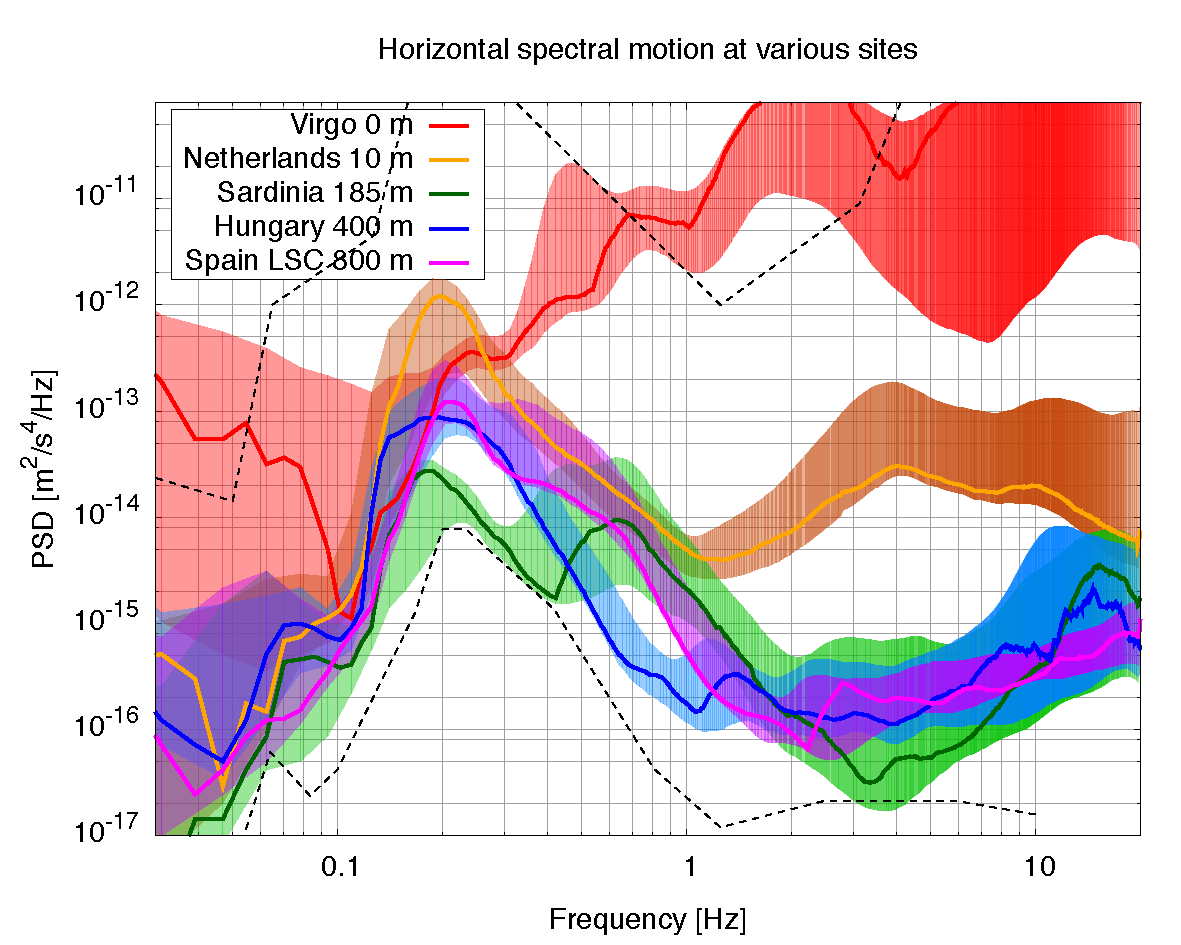
\includegraphics[width=14cm]{./Sec_SiteInfra/Figures/BestSiteComparison.png}
		\caption{Spectral variation results of the three candidate site, plotted for comparison is the site of the current GW detector Virgo. The solid lines correspond to the mode, while the upper and lower limits of the transparent regions are the PSD levels that weren't exceeded for 90 and 10 \% of the time respectively. }
		\label{fig:sitecomparison}
	\end{center}
\end{figure}

%%%%%%%%%%%%%%%%%%%%%%%%%%
\FloatBarrier
\subsection{Infrastructure realization}
\emph{
Responsible:  Jo v/d Brand \\
}

\subsubsection{Infrastructure overview}
Einstein Telescope will have excellent sensitivity of about $10^{-22}/\sqrt{\mathrm{Hz}}$ at low frequency (2\,Hz). This is achieved with advanced suspension systems with a frequency cut-off below 1.8\,Hz in combination with site locations that feature low seismic noise. Fig.~\ref{fig:candidates} shows that various excellent candidate sites for ET have been identified in Europe. ET will be constructed underground in order to benefit from low seismic and gravity gradient noise. It is well known~\cite{xx} that the major part of the seismic noise in the frequency range 1 to 10\,Hz is generated at the surface. The corresponding GGN is then partly suppressed at underground locations due to surface averaging effects. The GGN attenuation factor has been shown in Fig.~\ref{fig:ggnattenuation}. It is seen that GGN effects from surface waves can be attenuated by more than 2 orders of magnitude for frequencies $f > 2$\,Hz for underground detectors at moderate depth ($>100$ m) for soft-soil and homogeneous conditions. Dedicated studies~\cite{cellaggn} show that in general it will be a challenge to obtain sites with low GGN properties. FEA calculations reveal large differences in attenuation between 1 and 2 Hz. The required depth is driven partly by the wavelength of the seismic waves. Roughly $\lambda / 4$ is required for about a factor of 100 suppression. The wavelength scales with the seismic velocity. While for soft soil typical values of 440\,m/s are found for the longitudinal velocity $c_L$, these values increase to 6000\,m/s for stressed hard rock such as granite at great depth. Consequently, while the depth of ET could be limited to a few hundred meters when constructed in soft soil, significantly larger depths may be required when considering siting in hard rock. 

The ET site studies were performed at various underground locations in hard rock (Frejus, Canfranc, Gran Sasso, Sardinia and Hungary in Europe, Homestake in the USA, and Kamioka in Japan), in salt (Slanic Salt Mine in Romenia, and Realmonte in Sicily), and in Boom clay (the HADES facility for storage of nuclear waste in Mol, Belgium). The lowest seismic noise was obtained in hardrock. Note that homogeneity and seismic correlation length of the medium are expected to be important parameters for future GGN subtraction schemes.

The realization of ET requires the construction of substantial underground infrastructure. Fig.~\ref{fig:infra} shows an impression of the observatory.
\begin{figure}[htbp!]
	\centering
		\includegraphics[width=10cm]{./Sec_SiteInfra/Figures/infra.jpg}
		\caption{Artistic impression of Einstein Telescope. The observatory has a triangular configuration that can house three xylophone detectors. Each detector is comprised of a low-frequency cryogenic interferometer and a high-frequency interferometer operated at room temperature. The corner stations are connected by 11 km long tunnels.}
		\label{fig:infra}
\end{figure}

\begin{figure}[htbp!]
\centering
\includegraphics[width=11cm]{./Sec_SiteInfra/Figures/infra1.jpg}
\caption{Global layout of Einstein Telescope. Upper panel: during phase I the observatory will house a single xylophone detector. Lower panel: in phase II a triple xyolophone detector system will be implemented. Note that distances are not to scale.}
\label{fig:infra1}
\end{figure}
The observatory has a triangular topology that houses up to three xylophone detectors. The first phase of the project features a single xylophone configuration that consists of a cryogenic low-frequency interferometer and a room-temperature high-frequency  interferometer (see Fig.~\ref{fig:infra1}).

\begin{figure}[htbp!]
\centering
\includegraphics[width=14cm]{./Sec_SiteInfra/Figures/infra2.jpg}
\caption{Global view of a single xylophone detector showing the vacuum system and suspension towers needed to house the various optical components. Note that distances are not to scale.}
\label{fig:infra2}
\end{figure}

The three corner stations are connected by 11 km long tunnels. Each corner station
consists of a collection of surface buildings. The main assembly building gives
access to a 20 m diameter shaft that leads to the underground infrastructure.
At each corner there are three large experimental caverns, the main
cavern houses the laser injection systems and the beam splitters, while
both the end-test masses of the filter cavities for the high frequency beams
(ETM-FC-HF) and the input test masses of the filter cavities for the low
frequency beams (ITM-FC-LF) occupy the auxilliary caverns. 
Tunnels house the interferometer arms and have an inner diameter
of 5.5 m. In the following we discuss infrastructure aspects of 
the tunnels, underground caverns, and the vertical shafts and their construction.
In addition, we discuss issues encountered at other underground projects
and that may be of relevance for ET.

\subsubsection{Caverns}

\subsubsection*{Main caverns}

\begin{figure}[htbp!]
\centering
\includegraphics[width=23cm, angle=90]{./Sec_SiteInfra/Figures/infra3.jpg}
\caption{Schematic outline of the main infrastructure in one of the large underground caverns.
The labels are explained in the text.}
\label{fig:infra3}
\end{figure}
An outline of the detector system in one of the large
underground caverns is shown in Fig.~\ref{fig:infra3}. 
The cavern has a cylindrical shape with 65 m diameter and 30 m height.
It contains detector components from all three
xylophones (denoted by the last number on the labels). 
The laser of the low-frequency
interferometer for xylophone 1 is denoted LLF-1. It injects into the power-recyling mirror
PRM-LF-1 and is directed onto beamsplitter BS-LF-1. Arrows indicate the directions
of the two beams towards the 10 km long interferometer arms. In the same manner the
laser of the high-frequency beam of xylophone detector 1 is denoted LHF-1. It injects
the beam into PRM-HF-1 and then onto beamsplitter BS-HF-1. Again arrows indicate
the directions of the two beams. Steering mirrors, SM-HF-1, are used
to direct both HF beams towards the long interferometer arms. Steering mirrors are
used solely in the HF beams, since the requirements
for low-frequency seismic noise isolation are less stringent for HF beams than
for the LF beams. Both LF and HF beams use separate beam pipes. 
The LF beam is on top (in the vertical direction) of the HF beam as this approach
simplifies the cryogenic superattenuator design (see section xx).

The LF beam at the dark port ends on signal-recycling mirror SRM-LF-1. The light
is bounced off three steering mirrors, indicated in Fig.~\ref{fig:infra3} by
SM-SR-LF-1, and is directed towards a beamsplitter
at the entrance of filter cavity 1, BS-FC-LF1. Part of the light now enters the beam
tube of filter cavity 1, FC-1-LF-1, and falls on the injection test mass ITM-FC2-LF-1
located in the auxilliary cavern. FC-1-LF-1 is 10 km long and ends on the end test
mass ETM-FC-LF-1 located in the main underground cavern at the other side of the
interferometer arm.
The other part of the light enters a second filter cavity, FC-2-LF-1, and via
ITM-FC-2-LF-1 in the auxilliary cavern it enters the 10 km long filter cavity.
Again a test mass is located in the corner station at the other end. Both filter cavities use
separate beam pipes. The low frequency interferometer allows injection of
squeezed light (indicated in Fig.~\ref{fig:infra3} with label SLI). 

Also the HF beam at the dark port implements a filter cavity. Light from signal
recycling mirror SRM-HF-1 is reflected via steering mirror SM-R-HF-1 into the
injection test mass ITM-FC-HF-1 of the filter cavity. The cavity is 700 m long
and the end test mass ETM-FC-HF-1 is located in an auxilliary cavern.

Each main underground cavern houses two end test masses of both other
interferometers. In Fig.~\ref{fig:infra3} this is indicated by ETM-LF-2 and
ETM-LF-3 for the two other low-frequency interferometers, and by
ETM-HF-2 and ETM-HF-3 for the other high-frequency interferometers.
In addition, the main cavern houses the two end test masses of the filter cavities
for one of the other low-frequency interferometers. In Fig.~\ref{fig:infra3} this is 
indicated with ETM-FC-LF-3.

The main optical components of the interferometers need to be suspended.
Each main cavern houses 17 suspension towers; 4 of these towers are
part of the cryogenic suspension system needed for the suspension of the end
test masses of the two other LF interferometers.
Three towers are used to suspend double payloads, while three towers are used to
suspend triple payloads. In two cases the low frequency beam passes through
the suspension system of the high frequency beam. 

The main cavern is occupied by two cryolinks that protect the cryogenic
end test masses of both other interferometers from thermal radiation. In addition,
cryolinks are employed near the end test masses of the filter cavity of
one of the other interferometers. The cavern must accommodate the cryogenic infrastructure
needed for the operation of the four cryolinks.

It can be seen in Fig.~\ref{fig:infra3} that each main cavern is connected to
four tunnels. Two of these tunnels accommodate six vacuum beam pipes, 
a third tunnel holds the filter cavity for the high frequency interferometer,
and the fourth tunnel is empty. The latter is used to allow transportation
of equipment between main cavern and auxilliary cavern.

\subsubsection*{Auxilliary caverns}

\begin{figure}[htbp!]
\centering
\includegraphics[width=16cm]{./Sec_SiteInfra/Figures/infra4.jpg}
\caption{Schematic outline of the main infrastructure in one of the auxilliary underground caverns.
The labels are explained in the text.}
\label{fig:infra4}
\end{figure}

An impression of the infrastructure of one of the auxilliary
caverns is shown in Fig.~\ref{fig:infra4}. 
These caverns are cylindrical in shape with a diameter of 30 m and a
height of 30 m. In its final configuration, six beam pipes pass through this
cavern. The cavern is occupied by the input test masses of both the low
frequency and high frequency interferometer. The low frequency ITM is
a cryogenic payload and is surrounded with a cryolink. The cavern is
equipped with the necessary cryogenic infrastructure.
It can be seen in Fig.~\ref{fig:infra3} that each auxilliary cavern provides the
entrance to a main interferometer arm tunnel.

\subsubsection*{Cavern construction issues}

Einstein Telescope will have a total of 9 underground caverns. Each corner station
will have a large cylindrical underground cavern with a diameter of about 65 m and a
height of 30 m. Each corner station will have two smaller auxilliary caverns
with diameter and height of 30 m.

\begin{figure}[htbp!]
\centering
\includegraphics[width=12cm]{./Sec_SiteInfra/Figures/station.jpg}
\caption{The construction of the Robert Bourassa hydropower station in Quebec, Canada. 
Drill and blast was used ato excavate the powerhouse with dimensions 296 m by
25 m by 47 m. More than 11,000 rock bolts were used.}
\label{fig:station}
\end{figure}
ET's caverns will be constructed by the drill and blast (D\&B) technique. 
Worldwide various such large underground
structures have been constructed. Fig.~\ref{fig:station} shows the underground
hydropower station in Quebec (Canada). 

\begin{figure}[htbp!]
\centering
\includegraphics[width=16cm]{./Sec_SiteInfra/Figures/lhc.jpg}
\caption{The construction of the CMS cavern for the LHC project at CERN, Geneva.}
\label{fig:lhc}
\end{figure}
ET can profit from the large body of experience in underground cavern construction
for physics experiments. In particle physics there are LHC (previously LEP) at
CERN in Geneva, HERA at Desy in Hamburg, SLAC in Palo Alto and Fermilab in Chicago.
In addition, there are non-particle physics facilities as LNGS in Gran Sasso, LSM in Frejus, 
LSC in Canfranc, Kamioka in Japan and Dusel in South Dakota. 
Furthermore, there is experience from the mining industry.

As an example we show some of the experience in realizing large underground
caverns for the LHC project at CERN. These caverns host the Atlas and CMS experiments 
and have been constructed by D\&B. The left photo in Fig.~\ref{fig:lhc} shows the 
waterproofing foil used in the CMS
cavern at CERN. The right photo shows the completed cavern.
The Atlas cavern is located at a depth of 92\,m
and has a length of 55\,m, a width of 32\,m, and a height of 35\,m. The CMS
cavern is located at a depth of 20\,m and has a length, width and height of
53, 27, and 25\,m, respectively.

The construction of the Atlas cavern took 4.5 years and that of the CMS cavern 6.5 years. 
It is clear that for ET the various caverns must be constructed in parallel
in order to avoid excessive construction times.

\subsubsection{Tunnels}

The corner stations are connected by 10 km long tunnels. These tunnels
have an inner diameter of 5.5 m and an outer diameter of 6.5 m. At the location
of the cryolinks, the inner diameter will be increased to 6.0 m.
The main caverns and the auxilliary caverns are connected by a double
tunnel structure with a length of 700 m. 
Consequently, the observatory requires more than 34 km of tunnel.
  
The main interferometer arm tunnels accommodate six vacuum beam pipes.
In addition, the tunnel houses the services for electricity, water, compressed air,
cryogenics, safety systems and air conditioning. The diameter of the tunnel
is sufficiently large to allow transportation of vacuum beam pipes.
A sketch of the tunnel is shown in Fig.~\ref{fig:infra5}.
\begin{figure}[htbp!]
\centering
\includegraphics[width=17cm]{./Sec_SiteInfra/Figures/Tunnels1.pdf}
\caption{Schematic outline of the tunnel.
The tunnel is occupied by the vacuum vessels that hold the low frequency (LF-1 and LF-2)
and high frequency (HF-1 and HF-2) arms of two interferometers. In addition, the vacuum vessels
for both filter (FC-1-1 and FC-2-1) cavities are housed. The inner diameter is 5.5\,m and the tunnel
wall has a thickness of 50 cm.}
\label{fig:infra5}
\end{figure}
During installation the tunnel will be equipped with a monorail system.
This is used to transport the vacuum beam pipes. Provisions are made
to accommodate the large vacuum valves in the tunnel walls, and to allow
welding of the beam sections. For safety reasons the tunnel is divided
into 500 m sections that are equipped with fire retarding doors, and safety
shelters. The tunnel is equipped with an elaborate safety system that
allows control of the airflow in order to direct the smoke in case of a fire.

\subsubsection*{Tunnel construction}

At present there is a vast body of experience in tunnel construction.
This is to a large extent driven by the increasing worldwide demand 
for the creation of underground tunnels.
For the construction of high speed trains alone, in 2010
about 1000 km of lines is taken in operation, while the current demand
for 2020 is estimated at 3500 km \cite{itacet}.

\begin{figure}[htbp!]
\centering
\includegraphics[width=16cm]{./Sec_SiteInfra/Figures/tunneling.jpg}
\caption{Underground tunnels can be constructed with tunnel boring machines (TBM),
or by using the conventional drill and blast method (D\&B).}
\label{fig:tunneling}
\end{figure}

For the construction of underground tunnels, two major technical
approaches can be distinguished: tunnel boring machines (TBM) and
drill and blast (D\&B). Fig.~\ref{fig:tunneling} schematically shows
the two techniques.

\subsubsection*{Tunnel construction with TBMs}

The TBM technique is state of the art, and excavation rates of 20--25\,m per day
are routinely obtained. The geology must be well understood through site
surveys and one must realize that given the large size of the machine
(typically 400 m for the TBM and train combination) it is difficult to adapt to
changes (for example in geology). 

\begin{figure}[htbp!]
\centering
\includegraphics[width=14cm]{./Sec_SiteInfra/Figures/tbm.jpg}
\caption{Schematic representation of a gripper tunnel boring machine from Ref.~\cite{Herrenknecht}.}
\label{fig:tbm}
\end{figure}
Fig.~\ref{fig:tbm} shows an outline of a gripper TBM from Herrenknecht~\cite{Herrenknecht}.
This TBM has a 9.58\,m diameter and a length of 441\,m.  A power of 7.8\,MW is required
to drive the machine. The TBMs needed for ET would have a diameter of 6.5\,m.

The investment costs are large (e.g.\ about 20\,M\euro for the TBM shown in
Fig.~\ref{fig:tbm}) and set-up
times are long. In the case of ET several TBMs would be required in order to 
keep the construction time limited to 2 years. Sizeable diameters are needed for
the vertical shafts in order to lower the equipment. A typical TBM cycle would
involve boring 2 m of tunnel, followed by clearing out the rock. The tunnel wall support
with anchors, shotcrete and steel arches is then implemented next. Per day
shifts 1 and 2 would involve the above cycle, while shift 3 would be dedicated
to the service and repair of the TBMs.

\subsubsection*{Tunnel construction with D\&B}
 
The drill and blast technique is highly adaptable, but excavation rates are
limited to 6 - 10 m per day. A cycle consists of drill, charge, and detonate.
After ventilation, various tasks as support and muck removal take place. In good
rock conditions 1 cycle can be accomplished in an 8 hour shift.

\begin{figure}[htbp!]
\centering
\includegraphics[width=16cm]{./Sec_SiteInfra/Figures/multihead.jpg}
\caption{Special tooling has been developed for the D\&B technique for tunneling.}
\label{fig:multihead}
\end{figure}
In order to cope with the relatively low advance rate, various teams
have to work in parallel. Advanced multi-head drilling tools have been
developed (see Fig.~\ref{fig:multihead}) in order to increase the advance rate.
\begin{figure}[htbp!]
\centering
\includegraphics[width=10cm]{./Sec_SiteInfra/Figures/support.jpg}
\caption{Support of the tunnel walls can be erected in parallel to the drilling process.}
\label{fig:support}
\end{figure}
Fig.~\ref{fig:support} shows that support of the tunnel walls can be provided
in parallel with the multi-head drilling activities.

\subsubsection*{Practical experience with tunnel construction}

There is a vast amount of experience available with tunnel construction
in various soil types and under various conditions. When long tunnels (typically with
lengths exceeding 6\,km) are considered and smooth walls are needed
(e.g.\ for high speed trains) then TBMs are often selected. Underground
infrastructure such as train tunnels are designed for a lifetime of about
100 years. Thus, special wall treatment is needed to ensure such a long lifetime.

\begin{figure}[htbp!]
\centering
\includegraphics[width=11cm]{./Sec_SiteInfra/Figures/tunnelwall.jpg}
\caption{Wall segments used in the construction of the Gotthard-Basistunnel.
This project represents the world's largest underground construction.}
\label{fig:tunnelwall}
\end{figure}
Fig.~\ref{fig:tunnelwall} shows a wall segment that has been used in
the construction of the Gotthard-Basistunnel. The Gotthard-Basistunnel
represents the longest tunnel project in the world: a total tunnel length
of 98.135\,km has been constructed with TBM and 53.705\,km with D\&B. 
The lining is designed to handle corrosive water containing chloride,
sulphates, etc. The impermeable layer avoids swelling of the concrete,
corrosion of the anchors, and sintering in the drainage system.
The drainage system is designed to prevent groundwater pressure buildup.

\begin{figure}[htbp!]
\centering
\includegraphics[width=14cm]{./Sec_SiteInfra/Figures/rocktemp.jpg}
\caption{Rock temperature distribution in the Gotthard-Basistunnel.
Temperature is shown on the left vertical axis and depth on the right axis
(m.\"u.M = meters above sea level). Erstfeld, Amsteg, etc. are locations
along the tunnels.}
\label{fig:rocktemp}
\end{figure}
Construction of tunnels at large depth has various implications. Fig.~\ref{fig:rocktemp}
shows that in general rock temperature increases with depth. For train tunnels
these temperatures can be handled (since the trains act as pistons), but it may
cause troubles for ET. Sizeable and costly ventilation systems must be installed. These
systems also dilute dust and remove methane and radon (detection systems
for these gases must be installed). Other problems encountered in construction
at large depth include rockfall, rockbusts and possibly large deformations.

\begin{figure}[htbp!]
\centering
\includegraphics[width=12cm]{./Sec_SiteInfra/Figures/faido.jpg}
\caption{A seismic network set-up near Faido for the Gotthard-Basistunnel project
measured various micro tremors over a 2-year period.}
\label{fig:faido}
\end{figure}
For ET the issue of micro tremors may be significant. In the context of the
Gotthard-Basistunnel project, the Swiss Seismological Service, SED, recorded an
accumulation of seismic activity in the area of the MFS Faido (see Fig.~\ref{fig:faido}). 
Events were recorded in the period between March 2004 and June 2005. Normally, this
is a region with very low seismicity. A local seismic network was set-up at the 
multi-purpose station, MFS Faido, consisting of 9 stations at the surface, including one station from the
SDSNet. The stations were installed in a circular arrangement 10 to 15\,km
around the MFS Faido. In addition, 2 seismic stations were placed in the tunnel.
The hypocenters of the micro tremors were reconstruction in 3D. It was
clear that this seismicity was related to the underground tunnel construction.
The tremors were observed over at least a 2 year period.

\begin{figure}[htbp!]
\centering
\includegraphics[width=12cm]{./Sec_SiteInfra/Figures/dam.jpg}
\caption{Horizontal and vertical displacements measured at the water dam Nalps
are related to the Gotthard-Basistunnel project.}
\label{fig:dam}
\end{figure}
Several water dams are located in the vicinity of the Gotthard-Basistunnel.
TPS and GPS measuring systems were installed around these dams in order
to monitor surface ground motion. Fig.~\ref{fig:dam} shows that several
mm displacements have been measured at these dams. The movements
are correlated with the TBM activity at Nalps North and were first observed
in December 2005. It is believed that although these dams are several km away
from the underground construction, the movements are due to changes induced
in the ground-water levels.

In general the construction of the Gotthard-Basistunnel went according to
expectations. However, a major problem occured in 2003 when crossing the horizontal
fault zone at Bodio. The TBM got stuck for more than 6 months and had to
be excavated. This was possible since the project features 2 tunnels (an
East and a West railway tube).

TBMs can also be used to drill tunnels in
soft soil. In that case special types of TBMs (e.g.\ mixshield) must be used that have
a submerged wall, a working chamber, air cushion and pressure bulkhead. The
tunnel walls require advanced lining, while the TBM servicing requires special
manpower (divers). In general, tunnel construction in soft soil is considerably more expensive
than in hardrock.

The tunnel for the HERA ring (6.6\,km circumference) at DESY in Hamburg, Germany
and the LHC (the LEP) tunnel (26.7\,km circumference) at CERN in Geneva, Switzerland
have been constructed with TBMs. The 6 km tunnel for the LCGT project in the
Kamioka mountain in Japan will be constructed by D\&B. The ET team is in close
contact with LCGT and will more this project in detail over the next years.

\subsubsection{Shafts}

Presently, it is not clear whether ET will have horizontal or vertical access.
In the case of vertical access, there is a significant increase in complexity of the
construction methods needed for shafts with depths exceeding 200\,m. 

In the following, we present a discussion that is based on vertical access, similar
to for example the LHC experiment at CERN (see Fig.~\ref{fig:shaft}).

\begin{figure}[htbp!]
\centering
\includegraphics[width=12cm]{./Sec_SiteInfra/Figures/shaft.jpg}
\caption{The construction of the CMS access shaft for the LHC project at CERN, Geneva.
This shaft has an 18 m diameter and the entire CMS experiment was lowered through
it. To facility its construction, the ground at the shaft walls was frozen.}
\label{fig:shaft}
\end{figure}
Each corner station will be accessed through a 20 m diameter vertical shaft.
For excavation of the tunnels, the TBMs (in case this technique is adopted)
will be lowered through these shafts. After tunnel construction, the shafts
will be equipped with concrete elevator modules, staircases and will carry all
services (power, water, compressed air, ventilation ducts, etc.). Additional
shafts with a 10 m diameter are foreseen at the center of the arms.

\begin{figure}[htbp!]
\centering
\includegraphics[width=16cm]{./Sec_SiteInfra/Figures/cmsshaft.jpg}
\caption{Completed access shafts for the LHC project at CERN, Geneva.}
\label{fig:cmsshaft}
\end{figure}
The top of the shafts will be integrated in large suface buildings. There
the equipment of the ET interferometers, such as the vacuum system, will
be prepared. Subsequently, the various modules will be lowered through the
shafts into the caverns using hoisting devices.

\subsubsection{Final remarks}

Cost analysis shows that tunnels, shafts and caverns constitute the main cost drivers 
for the ET project. It is obvious that the cost of underground construction is site dependent
and contains large uncertainties at this stage of the project.

In follow up studies it is imperative that risk management of the project is assessed.
Worldwide many problems occured during underground construction. Furthermore,
in our discussions with insurance companies it became clear that part of the
risk cannot be insured (e.g.\ water leaks in tunnels). The Technical Committee on
Geotechnical Reports of the Underground Technology Research Council has
established guidelines for a so-called geotechnical baseline report (GBR) for construction.
It is customary that a project starts by defining such a GBR in order to establish
a baseline on risks (e.g.\ from geology) for industry and client. After
site selection such a GBR must be realized. It contains as much as possible detailed
site information based on geophysical surveys, lidar surveys, drilling samples,
probabilistic assessment of rock mass behavior, etc.\ and requires close collaboration
between the client, industry, and geophysicists.



\FloatBarrier
\subsection{Vacuum systems}
\emph{
Author(s): C.\ Bradaschia,  G.\ Parguez, A.\ Pasqualetti
}
% uncommented header -> document does not compile if that is still included (R. Nawrodt)

%\documentclass[11pt,a4paper]{article}
%\usepackage{verbatim}
%\usepackage[latin1]{inputenc}
%\usepackage[T1]{fontenc}
%\usepackage{ae}
%\usepackage{color}
%\usepackage{parskip}
%\usepackage{xspace}
%\usepackage[english]{babel}
%\usepackage{thumbpdf}
%\usepackage[pdftex,a4paper,pagebackref=true,pdfpagelabels=true]{hyperref}
%\definecolor{linkcolor}{rgb}{.8,0,0}
%\definecolor{urlcolor}{rgb}{0,0,.7}
%\definecolor{citecolor}{rgb}{0,.5,0}
%\definecolor{acrocolor}{rgb}{0,0,.7}
%\hypersetup{bookmarksopen,colorlinks=true}
%\hypersetup{pdfstartview=FitH}
%\hypersetup{linktocpage=true,bookmarksnumbered=true}
%\hypersetup{plainpages=false,breaklinks=true}
%\hypersetup{linkcolor=linkcolor,citecolor=citecolor,urlcolor=urlcolor}
%\usepackage{float}
%\usepackage{tabularx}
%\usepackage[pdftex]{graphicx}
%\usepackage{epstopdf}

%\usepackage{url}



%\title{ Vacuum Systems}
%\author{C. Bradaschia, G. Parguez, A. Pasqualetti\\ European Gravitational Observatory}

%\begin{document}
\FloatBarrier
\subsubsection{Vacuum Systems}


\paragraph{Introduction}  \label{intro}

In laser interferometers for GW detection most of the instrument has to be kept under High-Vacuum or Ultra-High-Vacuum (HV, UHV) for several reasons:
\begin{itemize}
\item reduce the noise due to vacuum fluctuations along the beam path to an acceptable level
\item isolate test masses and other optical elements from acoustic noise
\item reduce test mass motion excitation due to residual gas fluctuations
\item reduce friction losses in the mirror suspensions
\item contribute to thermal isolation of test masses and of their support structures
\item contribute to preserve the cleanliness of optical elements.
\end{itemize}


A vacuum system of this kind (Fig.~\ref{fig:vac1}) is composed of several UHV pipes with kilometric length and several cylindrical vertical HV/UHV tanks (towers) containing the optical elements and their support structures (Fig.~\ref{fig:vac2}). In general it is necessary to have the whole vacuum system constituting one single volume, without physical separations (windows) on the laser beam path. HV volumes (the towers) contain parts of the apparatus not easily compatible with UHV pipes where, on the contrary, the large majority of the laser beam has to travel. The separation between HV and UHV is obtained by differential pumping or by cryogenic traps, stopping the migration of water and other high vapor pressure components.

\begin{figure}
\begin{center}
\includegraphics[width=\textwidth]{Sec_SiteInfra/Figures/VAC1.pdf}
\caption{Schematic of the ET vacuum system lay-out, out of scale. Only one xylophone detector is shown, out of three.}
\label{fig:vac1}
\end{center}
\end{figure}

\begin{figure}
\begin{center}
\includegraphics[width=\textwidth]{Sec_SiteInfra/Figures/VAC2.pdf}
\caption{As an example the cross-section of a Virgo a mirror tower is shown.}
\label{fig:vac2}
\end{center}
\end{figure}


The vacuum enclosure will be built of stainless steel (304L); this material is preferred for its easy availability, its price, the large experience in machining and welding, the mechanical properties (ductility), the chemical properties and the achievable outgassing rate. The same choice has been made in the past for Virgo, LIGO, GEO600.



\paragraph{Average base pressure in the arm pipes} \label{average_pressure}

The noise due to vacuum fluctuations (index instabilities due to statistical fluctuations of the number of molecules in the volume occupied by the laser beam in the arms cavities) has been calculated by several people for Virgo and LIGO \cite{cella08}. It is (at first approximation) inversely proportional to the square root of the beam volume (or to the square root of the beam average radius or to the square root of the arm length or to the square root of the average pressure).
The following baseline parameters have been used:
\begin{itemize}
\item arm length:  					10 km
\item beam waist:  					40 mm (TEM00) @ 5 km
\item beam average radius on mirrors: 		120 mm
\item best sensitivity:  				$\sim 3\,10^{-25}$\,Hz$^{-1/2}$ @ 300\,Hz.
\end{itemize}


As it is common practice in matter of vacuum, we will take a safety factor of at least $10$ with respect to the pressure producing a phase noise at the limit of the best sensitivity. The residual gas composition will be dominated by hydrogen with presence of water and other gases; we will aim to keep the residual pressure at level of $1\,10^{-10}$\,mbar (H$_2$ and H$_2$O, each at $5\,10^{-10}$ mbar, would generate an overall noise level of about $2\,10^{-25}$ Hz$^{-1/2}$, see Fig.~\ref{fig:vac3}). The vacuum system will be extremely clean from heavy organic molecules, both to limit the phase noise and to prevent pollution of the optical components. Hydrocarbon partial pressure shall be at the level of $10^{-14}$ mbar.

\begin{figure}
\begin{center}
\includegraphics{Sec_SiteInfra/Figures/VAC3.jpg}
\caption{Phase noise given by selected gases compared to the expected sensitivity, computed for the appropriate beam profile. (Gas composition: Hydrogen [$1\,10^{-10}$ mbar], Water [$5\,10^{-11}$ mbar], Nitrogen [$1\,10^{-11}$ mbar])}
\label{fig:vac3}
\end{center}
\end{figure}


To reach these conditions it will be necessary:

\begin{itemize}
\item to fire (one week in an air oven at 450$^\circ$C) the stainless steel vacuum enclosure elements (or the raw material sheets) in order to reduce the H$_2$ outgassing rate at the level of $10^{-14}$ mbar l /cm$^{2}$ s
\item to bake for one week at $150^\circ$C the pipes already assembled and under vacuum in order to eliminate the water molecule layers sticking to the pipe inner wall.
\end{itemize}


Liquid nitrogen cryotraps will be necessary to separate the baked UHV pipes from the water dominated unbaked mirror towers, in HV regime. Concerning the phase noise, the path length of the beams in HV will be kept short, that is a negligible noise contribution, when compared to the kilometers in the UHV arm pipes.
Large gate valves will be put at each end of the arm pipes, in order to preserve vacuum when venting a tower. For the same reason each tower will be separable from the rest of the vacuum enclosure by suitable gate valves.
The reference cavities being less sensitive to vacuum noise require a residual pressure at the level of $10^{-7}$ mbar. Their pipes will not be fired at 450$^\circ$C nor baked at 150$^\circ$C.

\paragraph{The arm pipes}

Due to the multi interferometer/xylophone choice for ET, several beams will run along each side of the triangular tunnel, we assume four main beams and two filter cavity beams, taking into account all the three detectors (six interferometers) composing the full ET.

The chosen baseline configuration includes four pipes, one for each main beam: two with a $0.9$ m diameter for the HF interferometers and two $0.75$ m diameter pipes, for the LF interferometers. In addition, two $0.69$ m pipes for the two filter cavity beams belonging to each LF interferometer. HF interferometers will be equipped also with a 700 m long filter cavity, running in a dedicated tunnel, inside a 0.6 m diameter pipe.

The pipes will be arranged inside the tunnel cross-section as shown in Fig.~\ref{fig:vac4}: the filter cavities at the bottom, under a movable floor, the two HF beams on the floor at the tunnel sides and the two LF beams on top of them (see below the "Tower" paragraph).

\begin{figure}
\begin{center}
\includegraphics{Sec_SiteInfra/Figures/VAC4.jpg}
\caption{Arrangement of the vacuum pipes in the tunnel cross-section.}
\label{fig:vac4}
\end{center}
\end{figure}

The pipe construction procedure merges Virgo and LIGO experience, even if the final choice will be performed in due time, with the appointed company. The pipes will have thin walls (3 -- 4 mm) with external stiffening rings, every 1 -- 2 meters. Two ring s will be larger, serving as attachment for the supports (see below).

20 m long pipe elements will be fabricated by continuous spiral welding in a suitable clean factory installed on site. At one end of each element a suitable bellows will be added to accommodate thermal expansion, during bake-out; winter/summer temperature excursion should be negligible under ground. At both ends 2 mm thick lips will be added, to allow UHV compatible welding of adjacent elements, without inert gas protection on the inner side of the weld (this technique has been successfully applied in Virgo).

Simple supports ``a la LIGO'', using steel cables and adjustable stretching screws will be sufficient, coping with the relatively high stability of an under ground tunnel.

The pipes will be aligned in the tunnel using optical instruments and laser beams, since GPS will not be applicable under ground. The requested straightness error for the arms is of the order of 10 mm. Periodical surveys will be necessary every few years, in order to detect dangerous pipe displacements due to ground movements.

Each 10 km pipe will contain a few hundreds of metallic baffles for diffused light mitigation. They shall be made out of stainless steel with a suitable conical shape and serrated inner edge (Fig.~\ref{fig:vac5}) against diffraction. The radial width of the baffles, between 50 and 100 mm, and their position will be determined by a suitable simulation~\cite{vinet97,vinet96}.

\begin{figure}
\begin{center}
\includegraphics{Sec_SiteInfra/Figures/VAC5.jpg}
\caption{As an example the Virgo pipe conical baffles are shown.}
\label{fig:vac5}
\end{center}
\end{figure}


\paragraph{Pipe Assembly}

The $20$ m pipe elements will be lowered to the corner caverns with the ends sealed by suitable end-caps and equipped with thermal insulation; each element will weight about $1.5$ t. The element will be put on and bolted to a simple carriage made of two parallel $20$ m long beams supported by small train wheels. In this way pipe elements can be pushed to their position one after the other by an electric tractor running on $5$ km long rails reaching up to mid arm. The rails, two for each pipe, are supported by frames extending to the whole tunnel cross-section. These same frames have the function, as said before, of supporting the pipes.
In alternative the element could be suspended to a $20$ m long beam running, as a bridge crane carriage, attached to a $5$ km long rail. The rail, one per pipe, is supported by the already mentioned frames. Also in this case pipe elements can be pushed to their position one after the other by an electric tractor or by a traction line.

Every $500$ m, along the tunnel, there is an enlarged room to accept pumping, bake-out and control equipment; those rooms are used also to weld the pipe elements at ease in a wide area, under a clean tent.

The first pipe element is stopped with the rear end under the tent; when the front end of the second element is close, the sealing lids are removed, after starting appropriate clean air flows. The corresponding end lips of the adjacent elements are precisely adjusted and welded. The beams of the two carriages (under or above the pipe, according to the chosen option) are rigidly bolted together, taking care of appropriate compression/extension of the bellows.

The two modules are shifted forward until the rear end of the second module is at the welding position; now the front end of the third module is adjusted and welded as before. This procedure is continued until the $25^{th}$ module is welded and the $500$ m long section of pipe is completed.

The ends of the assembled pipe section are closed with vacuum tight lids, the section is evacuated and tightness tests are performed. The closing lids will be strongly fastened to the tunnel wall, in order to keep the $6.4$ t axial load due to atmospheric pressure.

The $500$ m long section will be then vented and shifted by $20$ m to its final position.

Every pair of upper support cables (as said, in the LIGO style) are attached to the corresponding support ring, the cables are tightened, the bolts of the pipe elements to the carriages are removed, the elements are lifted (lowered, in the case of suspended transportation) by $10$ mm in $1$ mm steps. The $500$ m long train composed by $25$ carriages is sent back to the end cavern, to start the assembly of the second $500$ m pipe section. The lower support cables are attached to the support rings and suitably tightened.

The clean tent and the welding equipment are transferred to the next enlarged room and the assembly of the second $500$ m pipe section is started. Once completed and vacuum tested, taking advantage of the bellows and of the support cables, the front lip of the new 500\,m section is adjusted to the rear lip of the previous section and welded. This final weld is the last to be performed in that particular enlarged room.

The procedure continues contemporarily extending the installed pipe from mid arm to both arm ends.

Concerning the pipes arrangement in the tunnel, it is necessary to have the possibility to inspect and repair the welds between pipe elements. This could be achieved leaving a clearance of about 0.5\,m between the ``nude'' pipes and the tunnel wall (at least every 20\,m). We should consider also the case of needs of (small) maintenance interventions on the tunnel wall lining.

A pumping station room is sketched in Fig.~\ref{fig:VAC7}. In practice it is an enlargement of the tunnel for a width of 12\,m and a length of 10\,m, allowing the installation of the pumps, which are hold in their position by a metallic frame not reported in the sketch. Three cabinets  housing the electronics of the vacuum equipment are included, together with an electrical power supply for baking (60\,VDC 300\,kW).

A bridge crane shall be present, and the room shall probably need a conditioned humidity and temperature, to allow electronics efficiency.

\begin{figure}
\begin{center}
\includegraphics[width=\textwidth]{Sec_SiteInfra/Figures/VAC7.jpg}
\caption{3D view of a pumping station: the blue objects represent the pumps and sensors, the yellow ones the cabinets for pumps control (1 per tube) and baking power supply (1 cabinet for all). A separate small room is reserved for the high voltage electrical transformer.}
\label{fig:VAC7}
\end{center}
\end{figure}


\paragraph{Pipe pumping system}

The pipe pumping system has been conceived to be composed of standard modules, grouped together, in order to limit the number of pumping stations along the arms.

The goal total residual pressure (hydrogen and other gases) of $1\,10^{-10}$ mbar can be obtained, after firing and bake-out (see a previous paragraph), with one 5000 l/s pumping group, every 500 m, both in a 0.9 m and in a 0.7 m diameter  pipe, the smaller gas load due to the smaller diameter being compensated by the relatively reduced conductance.

Below is described the pumping system for one single pipe. 

Each permanent pumping group will consist of three identical modules, each made of one 2500 l/s Ti sublimation pump (TSP), connected to the pipe through a 250 mm gate valve (the Ti will be sublimated not in the tube but in a separated chamber), coupled to a 300 l/s ion pump. The former to pump active gases, the latter to pump inert gases. At such a low pressure TSPs are expected to require not more than one yearly regeneration. NEG pumps are being considered as a possible alternative to TSPs. Some redundancy is necessary to cover the Ti pumps regeneration periods.

Besides the permanent pumping group, every pumping station will include suitable vacuum gauges and two 2000 l/s turbo, backed by a scroll pump, for initial evacuation and bake-out.

The Filter cavity pipes, requiring a $10^{-7}$ mbar residual pressure, will be equipped only with the turbo/scroll groups, possibly reinforced with $77$ K cryo-pumps.

Every 10 km pipe will have three RGA's, at each end and in the middle, to monitor the vacuum quality and for easier diagnosis in case of problems.

\paragraph{Pipe bake-out system}

In order to perform the 10 days bake-out under vacuum at 150$^{\circ}$C, the pipe could be heated by electrical current flowing in its walls, closing the circuit by a suitable Al bar or cable. Closing the circuit with the pipe of the adjacent twin interferometer would save the Al conductor cost, but does not seem practical. The use of DC will assure a uniform current and temperature distribution on the pipe walls and improve human safety. Typical arrangement of the circuit could be, similar to Virgo, a series of double ring circuits with one DC source every 500 m delivering 1000 A at 50 V along 250 m in each direction. Such a system will deliver 200 W per meter of pipe, which has been experimentally demonstrated to be sufficient to reach 150$^{\circ}$C, if the pipe is wrapped in a suitable 10-20 cm thick thermal insulation layer. Each DC source will consist of a transformer/rectifier supplied by medium voltage AC (15 kV). This choice is dictated to reduce the cross section of cables to distribute 2 MW along 10 km. 15 kV equipment will be confined in dedicated rooms.

In this configuration, delivering 300 W per meter of tunnel, in absence of ventilation, a very crude estimate considering a 6 m aperture tunnel, drilled in isotropic rocks (assumed  $\rho = 2500$ kg/m$^{3}$, k = 2.0 watt/m K, C = 800 joule/kg K) gives an increase of room and wall temperature by about +13$^{\circ}$C after a 10 days bake-out. This situation, being at the limit of what could be tolerable, suggests to exploit several remedies like baking at a lower temperature for more days and improving the thermal insulation properties, in order to reduce the temperature increase of the tunnel walls. A suitable air cooling system will be designed to reduce further the ambient temperature (possibly renewing once per hour the tunnel air volume). The overall power release inside the tunnel could be reduced also performing bake-out in sequence on shorter pipe sections, separated by ``pseudo-valves'', vacuum tight, but able to sustain null pressure difference.

\paragraph{Cryotraps}

As stated above, HV volumes (e.g.\ the towers) will communicate with the UHV pipe through liquid nitrogen cryotraps, to prevent migration of water and other high vapor pressure contaminants. In order to allow the beam passage the cryotraps will consist of a large hollow muff, containing liquid nitrogen, suspended inside an increased diameter pipe section, with a design very similar to the one adopted for LIGO, Virgo and Advanced Virgo (Fig.~\ref{fig:vac6}). The lateral surface will be thermally isolated by a few cylindrical metal screens; the heat exchange at both ends will be limited by suitable circular baffles, leaving passage for the beam. The propagation of mechanical noise due to liquid nitrogen bubbling will be limited installing cryotraps at least 20 m away from the mirror towers; this will help to avoid excessive cooling of the mirrors (to avoid condensation, in no circumstance a mirror should be the coldest point in the environment). Cryotraps will have valves at each end, in order to be confined during warming-up for regeneration (not more than once per year). The traps will be 7--10 m long for pipes with diameters of 0.6--1.0\,m. The liquid nitrogen consumption has been evaluated to be about 10 liters per hour per trap. In correspondence of the cryogenic towers for the 4 K mirrors of the LF interferometer, the cryotraps will be much longer (50\,m) and will include liquid helium sections to strongly limit the mirror heat exchange as described in the following section. We refer to the same section for a description of the supply plant for cryogenic liquids.

\begin{figure}
\begin{center}
\includegraphics{Sec_SiteInfra/Figures/VAC6.jpg}
\caption{A liquid nitrogen cryotrap.}
\label{fig:vac6}
\end{center}
\end{figure}

\paragraph{Towers}

Mirror towers upper part will have a 2--3\,m diameter to contain easily the pendulum chains of Superattenuators and the inverted pendulum legs; the structure will be an evolution of the Virgo towers~(Fig. \ref{fig:vac2}). The lower chamber of the towers will have a diameter up to 3\,m, to contain large payloads. The HF interferometer towers will have a large bottom lid to allow installation of payloads from a clean basement, under a filtered air shower. The height will be 10 m for the main mirrors of the warm HF interferometer. Auxiliary mirrors or benches requiring lower isolation, will be located in shorter towers. The towers containing the cryogenic mirrors of the LF interferometer, to achieve full seismic isolation performance down to 2\,Hz, will be up to 20\,m tall. In these towers, sitting on top of the HF interferometer, the payload installation will be performed through a lateral port. This order of superposition has been chosen to have the low power LF beam passing through the HF mirror suspensions (at room temperature) and not the high power HF beam passing through the low temperature LF mirror suspensions. The lower part of the cryogenic towers will be described in the next section. Each cryo-tower will be coupled to an ancillary tower to support the heat extraction chain preventing seismic noise propagation.

\paragraph{Tower pumping system}

Mirror towers will be made of two or three vacuum compartments in order to separate by differential vacuum the lower mirror chamber from the less clean suspension mechanics in the upper chamber. The horizontal separating walls will have a low conductance hole for the passage of the pendulum chain support wire. The mirror chamber will be equipped with a permanent pumping group consisting of one 2500 l/s Ti sublimation pump coupled to a 300 l/s ion pump. In addition one 2000 l/s turbo, backed by a scroll pump, will be operated for initial evacuation. The tower upper chamber(s) will be pumped by suitable turbo/scroll groups.

An effort will be performed to build the suspension mechanics and electronics with ultra clean and low outgassing components, in order to pump permanently also the upper chamber with ion pumps. The use of large cryo-pumps is being considered to increase pumping power and to eliminate moving parts from the vicinity of mirrors.

\paragraph{Valves}

A great number of UHV gate valves with large aperture, up to 1 m  will be necessary. They will be all metal with only the gate gasket out of vacuum outgassed Viton. Every tower will be separable from the rest of the vacuum system by such valves. Every cryotrap will also be separable for regeneration; the HV side will be equipped with a Viton gasket valve, while the UHV side will be equipped with a totally metallic ``pseudo valve'', vacuum tight, but tolerating only a few mbar pressure difference.




%\bibliographystyle{plain}
%\bibliography{vacbiblio}
%\end{document}


\FloatBarrier
\subsubsection{Cryogenic service infrastructures}
\emph{
Author(s): F.\ Ricci
}
We present two possible approaches for the cryo-plants to be set up mainly for the LF- Interferometer.
In fact the HF- interferometer includes just cryo-traps installed at the tube ends for fulfilling  the ultra high vacuum requirements. These traps already present in the LIGO detector and now planned also for  Advanced VIRGO,  are based on the use of liquid nitrogen. Similar cryotraps for the ET HF- interferometer have been already presented  in a previous section and from here after  we focus  on the cryogenic requirement of  the LF - interferometer.
The cryo-plant for the LF-interferometer  will provide  the refrigeration power needed to bring the mirror temperature  in the 4 K range. This porpoise can be pursued either by setting up a system based on a battery of cryo-coolers or in alternative using the classic approach of   liquid helium cryostats. In the next we sketch the main characteristics of  ET cryostats. Then we  present and compare the two alternative cryo-plants.


\subsubsection{The ET  cryostats}
\emph{Author: F.\ Ricci}

In order to reduce the thermal noise impact on the ET sensitivity curve its is sufficient  to cool at cryogenic temperature the four  test masses of the LF- detector. The heat is extracted from the mirror via the suspension fibers attached at the other end to the marionette.  Moreover  the marionette is suspended to the super attenuator which attenuates the seismic noise up to few hertz. Thus,  it is extremely important to preserve the mechanical isolation between the mirror and the cooler system. On the other hand   an efficient  thermal link between
the payload and the cooling system plays is crucial for  the design optimization: we have to 
design  links as short as possible and optimize the  thermal contacts,  in order to avoid 
refrigeration power loss. 
In figure~\ref{fig:cryo_infrastructure_figure/ET_main-cryostat} we report a sketch of the cryo-mechanical system to be adopted for ET-LF.


\begin{figure}[t!]
	\begin{center}
		\includegraphics[width=17cm]{./Sec_SiteInfra/Figures/ET_main-cryostat.pdf}
		\caption{Scheme of the cryostats needed for cooling a test-mass of the LF-interferometer.}
		\label{fig:cryo_infrastructure_figure/ET_main-cryostat}
	\end{center}
\end{figure}


The whole payload that we will describe in the suspension chapter is hosted in the lower part of the vacuum tower hosting the 17-m long super-attenuator chain.  The vacuum tower basement is a cryostat  with two thermal screens: the blue line schematizes a surface at $\sim4$\,K, while the red one is the shield at intermediate temperature ($\sim 80$\,K). The upper part and lower part of the tower are separated by a roof  crossed by the Ti-6Al-4V thin rod    which holds the whole payload\footnote{The interface between the upper and lower suspension is described in section~(\ref{Upper_lower_suspension_interface}.}.
The blue line define a volume that has to be vacuum tight. It will permit to cool and warm up faster  the whole payload by  adding pure Helium gas in this experimental volume. Few  mbars of helium   will provide an efficient heat exchange during the cooling phase of the payload from room to cryogenic temperature. Once  the equilibrium temperature is achieved, the helium gas is pumped out before  the laser light injection. 
The basement of the main tower hosting the mirror is connected to an ancillary tower  shown in the figure.
The ancillary tower is  hosting the cold box, which will keep the mirror at cryogenic temperature. The box can be either a simple liquid helium container in the case of a cryoplant based on cryofluids or the cold head of a cryo-refrigerator in the case of a cryocooler plant.

A  thermal line of 20 m maximum length connects the cold box to the last stage of the mirror suspension. It can be made of a  braid  of a high purity material as the electrolytic copper or the grade 6 aluminum (99.9999 \% purity). Both of them  are metals characterized by  thermal conductivity value of 2 kW/m/K in the range 1-10 K. In fact  a braid of   20 m length, made of 8 wires 1 mm diameter can support an heat flow of 200 mW for a temperature  difference  of$\sim$ 1K at the link ends.

To damp the vibration associated  to the cooling system, the soft braid is mechanically coupled to the auxiliary super attenuator chain, hosted in the ancillary tower and   fully complaint with the cryogenic environment. 


In order to define the requirement of  the cryo plant  we have to estimate the cryostat thermal inputs, which depend on the cryostat dimension and the quality of the thermal insulation. 

\noindent
Assuming  that the inner vacuum chamber has to host a mirror with a half meter diameter, we derived the order of magnitude of the thermal input  for the cylindrical cryostats whose dimensions are reported  in the following table:
\begin{table}[htp]
\caption{Cryostat dimensions}
\begin{center}
\begin{tabular}{|c|c|c|}
\hline
\hline
 Container & Diameter [m] & Height [m]\\
\hline
Payload vacuum chamber & 1.5 & 3  \\
Auxiliary tower  & 1 & 2 \\
\hline
\hline
\end{tabular}
\end{center}
\label{tab:cryostat_dimension}
\end{table}

 The thermal super insulation is a standard technique used in the modern cryostats.  The thermal  shield is formed by  highly heat reflective thin layers, set under vacuum  for increasing radiation reflection and decreasing radiation heat transfer through the insulation.  The  most known  implementation   is based on layers  of porous (self-vented) mylar  sheets, which are  aluminized on one side. The sheets are wrapped around the surface to be insulated and  form  a multilayer blanket. 
The mylar is an hydroscopic material incompatible with the HUV requirements of ET. As a consequence the proposed solution implies to  separate the chamber hosting the mirror to the insulation vacuum of the cryostat.   A dedicated pumping system ( rotary-roots-turbo-molecular group) will provide the vacuum insulation.  

Wrapping  25 and 75 layers of self vented aluminized mylar around the two thermal shield, we achieve   the condition to limit the thermal input 
below 1\,W for the 4\,K shields and  around  50\,W for the intermediate ones.
We assume in this evaluation  that the thermal input due to laser light absorbed by the mirror and the thermal radiation emitted by the the km tube is   in the range of few tens of milliwatts  thanks to low silicon absorption at the laser wavelength and to  the helium cryotraps described in~\ref{subsection_helium_cryotraps}. 

It is forth-worth to  evaluate in more details these data in the context of the ET technical design study.  
\FloatBarrier
\subsubsection{The LF-interferometer cryotraps}
\label {subsection_helium_cryotraps}
\emph{
Author(s): G.\ Gemme}
\paragraph{Motivations.\newline}

\etbox{h}{box:intro}{Thermal radiation}{All substances continuously emit electromagnetic radiation by virtue of the molecular and atomic agitation associated with the internal energy of the material. The emitted radiant energy can range from radio waves, which can have wavelengths of tens of meters, to cosmic rays with wavelengths less than $10^{-14}$\,m. In this paragraph we will consider only radiation that is detected as heat. Such radiation is termed \emph{thermal radiation}; it occupies the intermediate frequency range between approximately $10^{-6}$\,m and $10^{-3}$\,m. Radiation from the warm surfaces to the cold surfaces is the dominating mode of heat transfer in vacuum.}

The main heat inputs into the cold mirror of the LF interferometer are the thermal radiation coming from the warm surface of the vacuum tube, and the heat load due to the  absorption of a small fraction of the laser light into the mirror surface. The latter can be estimated considering that the laser power circulating in the optical cavity is 18\,kW, and that a reference value for the absorption coefficient of the mirror optical coating at the working wavelength is around 1\,ppm. This gives an approximate value of 20\,mW of absorbed laser power.

The radiation from the warm surface of the vacuum tube to the mirror can be estimated by the modified Stefan-Boltzmann equation:
\begin{equation}
\label{eq:Stefan-Boltzmann}
\dot{Q_r}/A_1 = \sigma F_e F_{1-2} (T_2^4 - T_1^4)
\end{equation}
where $\dot{Q_r}/A_1$ is the heat transfer rate by radiation per unit area of the mirror surface, $\sigma=5.67\,10^{-8}\, \mathrm{W/m^2/K^4}$ is the Stefan-Boltzmann constant, $F_e$ is the emissivity factor, and $F_{1-2}$ is a geometric configuration factor relating the two surfaces, whose temperatures are $T_2$ (warm) and $T_1$ (cold).  From Eq.~\ref{eq:Stefan-Boltzmann} the heat flux on the mirror at $T_1 = 10$\,K, coming from the vacuum tube at $T_2 = 300$\,K can be as high as $\dot{Q_r}/A_1\sim 460\,\mathrm{W/m^2}$. This huge heat flux is not compatible with the cryogenic environment and needs to be reduced by several orders of magnitude. 

In order to reduce the thermal radiation from the beam duct into the cold mirror, two strategies are viable, as shown by Eq.~\ref{eq:Stefan-Boltzmann}: the reduction of the emissivity factor and/or the reduction of the geometric configuration factor, i.e.\ the reduction of the solid angle under which the warm surface is seen by the cold surface.

The emissivity factor can be reduced by an appropriate choice of material for the wall of the tube, or trough the deposition on the warm surface of a low-emissivity coating. The reduction of the geometric configuration factor, on the other hand, can be obtained by building in the region adjacent to the mirror cold sections of the vacuum tube (thermal shields or cryotraps), that ``move away'' the warm section of the tube from the mirror, and in this way reduce the solid angle under which the warm surface is seen by the cold mirror.  The temperature(s) and length(s) of these sections must be chosen in order to minimize the ration heat transfer to the mirror, and, at the same time, the overall cost of the cryogenic plant. Moreover, they will also serve as cryogenic pumps. In particular, in the region immediately adjacent to the mirror, a zone \emph{colder} than the mirror itself is needed to avoid the condensation of the residual gas on the surface of the mirror, that could lead to the growth of a layer of contaminants and spoil its optical characteristics.
 
\paragraph{Maximum heat load on cryogenic mirror.\newline}

The equilibrium temperature of the mirror is reached when the power extracted by the cooling system is equal to the power absorbed by the mirror ($\dot{Q}_{abs}=\dot{Q}_{coolsys}$). The power extracted by the cooling system mostly flows through the four silicon suspension wires (a small fraction is exchanged with the surroundings through thermal radiation) to the penultimate mass (the marionette) and then is removed by the heat sink directly connected to the cooling system.
The equilibrium temperature of the mirror $T_{mir}$ can be calculated by a simple analytical model if we assume that the temperature of the penultimate mass is kept fixed at the design value of 5\,K:
\begin{eqnarray}
\dot Q_{abs} & =  & \frac{4  S_w}{L}<k_{Si}>\left (T_{mir} - T_{mario}\right) \\
 <k_{si}> & = & \frac{1} {{\Delta T}}\int\limits_{T_{mir}}^{T_{mario}} {{k_{si}}(T)_{}^{}dT}
\end{eqnarray}
where $S_w$ is the section of the silicon suspension wire, $L$ is its length and $k_{si}(T)$ is the thermal conductivity of silicon. In the following calculations we shall use the thermal conductivity shown in Fig.~\ref{fig:k-silicon-comsol}~\cite{k-silicon-comsol}. From this figure we see that $<k_{si}>\sim 1.4\, 10^3 \, \mathrm{W/m/K}$  in the temperature range of interest (5--10\,K). We also take the design values for the silicon suspension wires (diameter: 3\,mm, length: 2\,m). The maximum power that can be extracted from the mirror, keeping its temperature at the design value of 10\,K, is approximately 100\,mW. 
\begin{figure}[htbp]
	\begin{center}
		 \includegraphics[width=12cm]{Sec_SiteInfra/Cryotraps/k-silicon-comsol.pdf}
			\caption{Thermal conductivity of silicon  (from \cite{k-silicon-comsol})}		
			\label{fig:k-silicon-comsol}
	\end{center}
\end{figure}
Since the laser power absorbed by the mirror is approximately 20\,mW, we can conclude that the thermal radiation heat load must not exceed $\sim$ 80\,mW.

%\paragraph{Heat load on cryogenic mirror -- finite element model.}
The above back-of-the-envelope calculation was checked by a finite element model of the mirror and its suspension system, as shown in Fig.~\ref{fig:model}
\begin{figure}[htbp]
\begin{center}
 \includegraphics[width=12cm]{Sec_SiteInfra/Cryotraps/model.pdf}
			\caption{Finite element model and boundary conditions}
\label{fig:model}
\end{center}
\end{figure}
The parameters used in the model are summarized in table~\ref{tab:model-parameters}.
\begin{table}[htbp]
\caption{Finite element model parameters}
\begin{center}
\begin{tabular}{|l|l|}
\hline \rule[-2ex]{0pt}{5.5ex} Mirror temperature & 10\,K \\ 
\hline \rule[-2ex]{0pt}{5.5ex} Mirror diameter & 45\,cm \\ 
\hline \rule[-2ex]{0pt}{5.5ex} Mirror mass & 211\,Kg \\ 
\hline \rule[-2ex]{0pt}{5.5ex} Silicon fibers length & 2\,m \\ 
\hline \rule[-2ex]{0pt}{5.5ex} Silicon fibers diameter & 3\,mm \\ 
\hline \rule[-2ex]{0pt}{5.5ex} Marionette temperature & 5\,K \\ 
\hline \rule[-2ex]{0pt}{5.5ex} Power in cavity & 18\,kW \\ 
\hline \rule[-2ex]{0pt}{5.5ex} Absorbed power  & 20\,mW \\ 
\hline \rule[-2ex]{0pt}{5.5ex} Beam radius & 9\,cm \\ 
\hline 
\end{tabular} 
\end{center}
\label{tab:model-parameters}
\end{table}

The calculation was done setting on the front surface of the mirror a fixed heat source, representing the power coming from the laser and absorbed by the mirror, of 20\,mW, with superimposed a variable heat source, representing the additional heat load due to thermal radiation. For the sake of simplicity the temperature of the penultimate mass was set at the fixed value of 5\,K.  The thermal conductivity of silicon shown in Fig.~\ref{fig:k-silicon-comsol} was used in the model~\cite{k-silicon-comsol}.

The solution of the problem was calculated sweeping the variable heat source in the 0--0.1\,W range, with steps of 10\,mW, and looking at the temperature in the central area of the mirror. The results are shown in Fig.~\ref{fig:T-mirror-0-100}. They confirm the order-of-magnitude values found in the previous section. The temperature of the central area of the mirror does not exceed 10\,K when the thermal radiation is lower than 70\,mW, corresponding to 90\,mW of total power absorbed by the mirror.
\begin{figure}[htbp]
\begin{center}
 \includegraphics[width=12cm]{Sec_SiteInfra/Cryotraps/T_mirror-0-100.pdf}
			\caption{Temperature at the center of the mirror vs.\ thermal radiation power}
\label{fig:T-mirror-0-100}
\end{center}
\end{figure}

\etbox{r}{box:maxpower}{Maximum thermal radiation power on cold mirror}{The maximum power that the mirror can absorb, keeping its temperature at the fixed value of 10\,K is approximately 90\,mW. Since the power absorbed from the laser is 20\,mW, the thermal radiation power must not exceed 70\,mW. In order to reduce the thermal radiation from the beam duct into the cold mirror, two strategies are viable: the reduction of the emissivity factor and/or the reduction of the geometric configuration factor, i.e.\ the reduction of the solid angle under which the warm surface is seen by the cold surface. The reduction of the geometric configuration factor can be obtained by building in the region adjacent to the mirror cold sections of the vacuum tube, that ``move away'' the warm section of the tube from the mirror, and in this way reduce the solid angle under which the warm surface is seen by the cold mirror.} 

In the following paragraph we shall find out how to design the thermal shields in the region adjacent to the mirror to keep the thermal radiation from the warm surface of the vacuum tube at a value not greater than few tens of milliwatts.

\paragraph{Thermal radiation from vacuum tubes - Direct exchange. \newline}

Radiative transfer of heat from one area to another depends, among
other things, upon the fraction of the radiant energy emitted by one area
which is intercepted by a second area. This fraction is identified by
several names, such as the configuration factor, the interchange factor,
the angle factor, or the geometric view factor, and is a function of the
geometrical relation of the areas involved. The configuration factor is defined as the fraction of diffusely radiated energy leaving surface A that is incident on surface B, and it is represented by the $F_{1-2}$ factor that appears in Eq.~\ref{eq:Stefan-Boltzmann}. 

We have to explicitly calculate the configuration factor for the geometry schematically shown in Fig.~\ref{fig:vacuum-tube}
\begin{figure}[htbp]
\begin{center}
 \includegraphics[width=12cm]{Sec_SiteInfra/Cryotraps/vacuum-tube.pdf}
			\caption{Conceptual scheme of the vacuum tube with cryotraps}
\label{fig:vacuum-tube}
\end{center}
\end{figure}

The details of the calculation are presented in Appendix~\ref{sec:geometric-appendix}. Making use of Eq.~\ref{eq:Stefan-Boltzmann} we can calculate the thermal radiation power on the mirror as a function of the lengths of the two cold sections, at 4.2\,K and 77\,K. The result is shown in Fig.~\ref{fig:contour}
\begin{figure}[htbp]
\begin{center}
 \includegraphics[width=12cm]{Sec_SiteInfra/Cryotraps/contour.pdf}
			\caption{Thermal radiation on the mirror vs.\ lengths of 4.2\,K and 77\,K sections.}
\label{fig:contour}
\end{center}
\end{figure}

\etbox{r}{box:cryolength}{Lenghts of the cryotraps}{We see that to keep the thermal radiation power in the range $\sim 10$\,mW, we need a 4.2\,K section of few meters and a 77\,K section of few tens of meters. For example, with $L_{4.2}=10$\,m and $L_{77}=50$\,m, we are in a situation were the \emph{direct} transfer of thermal energy from the warm tube to the mirror is approximately 3\,mW, well below the maximum allowed value.}

\paragraph{Thermal radiation from vacuum tubes - specular and diffuse reflection.\newline}
\etbox{h}{box:specdiff}{Specularly and diffusely reflecting surfaces}{The calculation of the thermal energy \emph{directly} transferred from the warm surface to the cold mirror is not sufficient. For the correct evaluation of the thermal radiation on the cold mirror reflections along the cryo-shields including the reflective properties of the surfaces must be taken into account.  These are rather difficult to specify as the reflected energy depends not only on the angle at which the incident energy impinges on the surface but also on the direction being considered for the reflected energy.  Two important, and relatively simple, limiting cases can be used for calculating heat exchange: \emph{diffuse} surfaces and \emph{specular} surfaces. In specular reflection, also called mirror like reflection, the propagation direction of the radiation is not significantly changed, whereas in the case of diffuse reflection the reflected radiation is reflected into all directions. An ideally diffusely reflecting surface will have will equal luminance for all directions.}

For a diffuse surface the incident energy from the direction $(\theta, \phi)$ that is reflected produces a reflected intensity that is uniform over all $(\theta_r, \phi_r)$ directions. When a diffuse surface element irradiated by an incident beam is viewed, the element appears equally bright from all viewing directions.  In the previous paragraphs, all the surfaces involved in the calculation of the configuration factors---in particular the inner surface of the vacuum tube---were assumed to be diffuse emitters.

Mirror-like, or specular, surfaces obey well-known laws of reflection. For an incident beam from a single direction, in a specular reflector, the reflected beam is at the same angle away from the surface normal as the incident beam, and is in the same plane as that formed by the incident beam and surface normal. When reflection is diffuse, the directional history of the incident radiation is lost upon reflection. With specular reflection the directional history of the incident radiation is not lost upon reflection. Consequently, when dealing with specular surfaces, it is necessary to account for the specific directional paths that the reflected radiation follows between surfaces.

An important parameter for deciding whether a surface falls in the diffuse or specular limit is the surface roughness, or more precisely the ratio of the root-mean-square roughness to the wavelength of the radiation. For long-wavelength radiation a smooth surface tends toward being optically smooth, and the reflections tend to become more specular. Thus, although a surface may not appear mirror-like to the eye (i.e.\ for the short wavelengths of the visible spectrum), it may be specular for longer wavelengths in the infrared.

The contribution to the thermal radiation heat transfer coming from \emph{diffuse} reflectivity was calculated for the geometry given in Fig.~\ref{fig:vacuum-tube} by a finite-element model (for the details see Appendix~\ref{sec:diffuse-appendix}). The geometric dimensions of the system were the same as in table~\ref{tab:model-parameters}, with the lengths of the cold sections $L_{77}= 50$\,m and  $L_{4.2}= 10$\,m. The results are shown in Fig.~\ref{fig:q_eps_diffuse}:
\begin{figure}[htbp]
\begin{center}
 \includegraphics[width=11cm]{Sec_SiteInfra/Cryotraps/q_eps_diffuse.pdf}
			\caption{Thermal radiation heat transfer in the diffuse reflection limit}
\label{fig:q_eps_diffuse}
\end{center}
\end{figure}

The case when the pipe walls are specularly reflecting was discussed in~\cite{tomaru_2007, tomaru_2008}. A large heat load caused by thermal radiation through a metal shield pipe was observed in a cooling test of a cryostat for a prototype of the cryogenic
interferometric gravitational wave detector (CLIO) in Japan. The heat load was approximately
three orders of magnitude larger than the value calculated by the Stefan-Boltzmann law. The phenomenon was studied both by simulation and by experiment and it was found that found that it was caused by the conduction of thermal radiation in a metal shield pipe due to multiple specular reflections in the pipe. 

A simple model for the evaluation is illustrated in Fig.~\ref{fig:specular}~\cite{mosher_1976}.
\begin{figure}[htbp]
\begin{center}
 \includegraphics[width=11cm]{Sec_SiteInfra/Cryotraps/specular.pdf}
			\caption{Thermal radiation "light-pipe" geometry for an on-axis source}
\label{fig:specular}
\end{center}
\end{figure}

In the case we are considering the aspect ratio of the pipe is sufficiently large to make the number of reflections
\begin{equation}
N \sim \frac{L}{d} \tan \theta	
\end{equation}
a number large compared to unity. At each reflection the radiation intensity is reduced by an amount $\rho(\theta)=1-\epsilon$ the specular reflection coefficient of the wall. The total reduction in intensity due to reflections at a given angle of incidence in the tube is determined by $\rho^N$.

The efficiency of transfer of radiation, $\eta$ emitted by an on-axis point source is then
\begin{equation}
\eta = \int_0^{\frac{\pi}{2}} \rho^N \sin \theta \, d\theta
\end{equation}
The plot of the radiation heat transferred to the mirror by specular radiation is shown in Fig.~\ref{fig:q_eps_specular}.
\begin{figure}[htbp]
\begin{center}
 \includegraphics[width=10cm]{Sec_SiteInfra/Cryotraps/q_eps_specular.pdf}
			\caption{Thermal radiation heat transfer in the specular reflection limit}
\label{fig:q_eps_specular}
\end{center}
\end{figure}

\etbox{r}{box:diffheat}{Heat transfer from diffusely and specularly reflecting surfaces}{We see that for $\epsilon \geq 0.1$ the heat transferred to the mirror is essentially the direct contribution from the warm tube. Only for small values of $\epsilon < 0.1$ (high reflectivity $\delta > 0.9$) the contribution to the heat transfer from the surface reflectivity increases dramatically. On the other hand, we see that for specularly reflecting surfaces a huge amount of heat reaches the mirror for almost all the values of the emissivity. Specular reflections inside the vacuum pipe must be strongly suppressed.}

\paragraph{Mitigation strategies.\newline}
\begin{itemize}
\item{The \emph{direct} radiation heat from the tube at 300\,K to the cold mirror is strongly suppressed with cold sections (cryogenic shields, or cryotraps) near the mirror. With a section 10\, m long, cooled at liquid helium temperature, and a section 50\, m long, cooled at liquid nitrogen temperature, the direct heat transfer can be reduced in the milliwatt range.}
\item{For the given cold pipe aspect ratio $L/d \sim 80$, the contribution of \emph{diffuse} reflectivity of the surface of the cold sections becomes important only for reflectivity $\delta > 0.9$ ($\epsilon < 0.1$).}
\item{Specular reflection in the cryogenic shields can increase the radiation heat transfer by two or three orders of magnitude. The effect can be controlled by placing absorbing baffles on the radiation paths inside the cold pipe; by coating the inner surface of the cold pipe with an high emissivity layer ($\epsilon > 0.9$); increasing the surface roughness of the cold pipe to suppress the mirror-like reflections} 
\end{itemize}


%According the guide lines described above, the overall design of the mirror  suspension and its control system will be very different from those ones presently   used in interferometric antennas. The new system will be the result of a trade off between the need to have a strong thermal contact with the cooling system and the tentative to reduce any dissipation source due to the coupling of the suspension with the mirror.
\FloatBarrier
\etbox{h}{box:information}{The Pulse Tube cryocooler} {The Pulse Tube cryocooler (PT) is based on the displacement and the expansion of a gas, usually helium (He$^4$).  A piston compressor and a rotary valve  are used to create the pressure oscillations ( the typical average pressure in a PT is $10^{�25}$ bar, and the oscillation amplitude is ranging between $2$ and  $7$ bar). Let us refer to the figure \ref{fig:PT_scheme} for explaining the thermal process.
\begin{figure}[H]
	\begin{center}
		\includegraphics[width=9.5cm]{./Sec_SiteInfra/Figures/PT_scheme.pdf}
		\caption{Scheme of a Pulse Tube cryocooler.}
		\label{fig:PT_scheme}
	\end{center}
\end{figure}
We note that  a crucial element of the cryocooler is the  PT regenerator,  a heat exchanger acting as {\it cold storage} systems for the  pulsed flow process.   In practice, the regenerator  stores the energy from one stream and later transfer the energy to a second stream, for example between the out-of-phase pulses of gas. \\
The orifice 1  is connecting  the warm end  to a buffer volume, ten times larger than the volume of the pulse tube so that its pressure is almost constant and close to the average pressure in the pulse tube. The combination of the orifice and the buffer provides a phase difference between the flow of the gas in the tube and the pressure oscillation; such phase difference is necessary for optimizing the PT performance \cite{Mikulin}. The function of the second orifice  is to reduce losses allowing some gas to bypass the regenerator \cite{Zhu} .
\begin{itemize}
\item{When the pressure rises, the gas element moves through the regenerator in the direction of the cold heat exchanger. At the regenerator output  the temperature of the gas element is $T_c$ and enters the tube. There, the gas element is compressed adiabatically, while it moves towards the orifice and  Its temperature rises together with the pressure.}
\item{Now, the orifice 1 is open and  the gas  at pressure $p_h$ flows from the tube to the buffer since  the buffer pressure is lower than that of the tube.}
\item{ The orifice 1 is closed and the rotary valve is set to connect the system to the low-pressure side of the compressor ($p_c$). The gas moves back to the cold heat exchanger and the expansion takes place.  At the end of the expansion step, the pressure of the gas element is equal to $p_c$  and theits temperature is below $T_c$.}
\item{The expansion stops, and the orifice is open again. The gas continues to flow in the direction of  cold heat exchanger and when it is crossing it , the gas warms up to the temperature $T_c$. The amount of heat, which the gas takes away from the heat exchanger, is the cooling power.}
\end{itemize}
To obtain temperatures below 20 K, the system is  operated at low frequency ( $\sim 1$ Hz ).
The frequency defines the diffusion depth $\delta$ in the working gas and the regenerator material:
$$d = \sqrt{\frac {k}{\pi \nu C}}$$
\noindent where $k$ is the heat conductivity, $\nu$ is the frequency and $C$ is the volumetric heat capacity of the regenerator material. Thus, it follows that when the frequency is increased, the diffusion depth decreases, and the heat storage in the regenerator degrades.
Moreover, a high operating frequency leans to a large pressure drop in the regenerator, i.e. a poor performance of a system.}
\FloatBarrier
 \subsubsection{The cryogenic infrastructure based on pulse tube cryo-coolers}
 \label{sec:cryocoolers}
\emph{
Author: F.\ Ricci}

A simple approach to cool down the mirrors  is based on the use of cryocoolers~\cite{LCGT}. In particular,  
Gifford-McMahon (GM) refrigerators have been developed since a long time and are widely used in various fields of science and industries because of their convenient handling. 
However, their cooling power  is provided by the motion of a displacer which causes large vibrations at the cold head, an aspect which makes them not suitable for all applications where a low acoustic noise level is necessary.

In more recent times,  the pulse tube (PT) cryocoolers  have been developed. 
The particular thermal cycle of PT refrigerators gives them a  two or three  times higher efficiency than GM cryocoolers for loads temperatures between 55 and 120 K, and requires no moving elements at low temperature. This latter characteristic is quite important: because of it, we expect PT refrigerators to be intrinsically more reliable and less noisy than classic GM coolers  \cite{japanoise}. 
Thus, a pulse tube cryocooler seems to be an interesting option for our purposes. However,  because of the gas pulse flowing in its cold head, also this kind of refrigerator injects mechanical noise in the cooled sample, at a level which is still far too high for the elements of a gravitational antenna. Indeed, in order to detect gravitational waves, current detectors have reached displacement 
sensitivities of the order of $10^{-18} m/\sqrt(Hz)$ and an increase by at least two orders of magnitude  is foreseen for ET, where we have to implement the use of low temperatures.

 
 The starting point of the system design is the choice of the pulse tube refrigerator model.
We compared two different models of cryo-coolers, the Cryomech PT 407 and the Sumitomo SRP-052A. For both systems, we measured the acceleration of the $4$ K cold head.

\begin{figure}[t!]
	\begin{center}
		 \includegraphics[width=12cm]{./Sec_SiteInfra/Figures/Sumitomo_Cryomech.pdf}
		\caption{The displacement noise spectrum of the second stage cold point of the CRYOMECH PT407 and of the Sumitomo SRP-052A as function of the frequency.}
		\label{fig:sumitomo_cryomech}
	\end{center}
\end{figure}



Our data show that the vibration noise level generated by the Sumitomo is lower by a factor $\sim 10$ than that by the Cryomech. 
Moreover, our model of Sumitomo has the additional advantage of having the room temperature throttle valve separated from the main body of the refrigerator, with the possibility to keep it far from the cryostat obtaining a further attenuation of the noise produced by this element.
However, the first harmonic generated by the pulse tube is around 1 Hz and it is not attenuated efficiently by the super attenuator chain.  In order to overcome this difficulty, the plan is to apply the technologies developed for  gravitational interferometers and to reduce the vibrations of the cold finger of a PT  cryocooler by an active control system.  In the past we  designed a vibration free cryostat~\cite{VFC}  for limiting the cryocooler vibration, according to the issues discussed above.  The cryostat scheme is sketched in  figure~\ref{fig:cryostat_scheme}.  It is based on the idea to attenuate the cryocooler vibrations by directly acting on it. 
 The cold head vibration  is monitored by  an  optic bundle fiber, a displacement sensor acting as low temperature,  while the actuation is based  on three piezoelectric stacks set  at room temperature outside the cryostat vacuum.  
The cryocooler cold head is clamped to a platform placed on dampers and it is connected to the cryostat by a soft  bellow designed to mechanically decouple it from the cryostat. The feedback correction signal is sent to the three piezo-actuators which are loaded by the platform and can push the cold head platform elastically coupled to cryostat mechanical structure.

\begin{figure}[htbp]
\begin{center}
\includegraphics[width=9cm, height=9.9cm]{./Sec_SiteInfra/Figures/cryostat_scheme.pdf}
\caption{{A simplified scheme of the vibration free cryostat.}}
\label{fig:cryostat_scheme}
\end{center}
\end{figure}


At present the attenuation achieved controlling just the vertical degree of freedom is of the order of $3 \cdot 10^{-3}$.  A further improvement is expected by controlling the horizontal  degrees of freedom and by reducing the recoil effect on the structure holding the monitor sensor of the 4\,K stage. However this active attenuation system is not sufficient and in parallel to this R\&D effort  industrial studies a are under way~\cite{Riabzev} ,  new proposals  have been presented \cite{Suzuki_2006}  to reduce the  the cryo-cooler vibration. We discuss  some of new ideas in the R\&D section~\ref{cryo_infrastructure_R&D}.

The  cryo-plants based on PT cryo-coolers implies to install for each tower hosting a test mass a doublet of one stage and two stage PT  cryocoolers. A similar solution is used  to cool the ancillary tower. It will permit to speed up the cooling process  providing  a redundancy during the data taking phase. 
Each PT cold head is driven by a  helium compressor via a couple of high pressure flexible line of a maximum length of 30\,m. 
A larger number of cryocoolers ($\sim 10$) are needed for the helium cryotraps (see~\ref{subsection_helium_cryotraps}).
Each compressor  operates at a pressure $\sim 22$ bar, it requires 5\,l/min of refrigerated water and it absorbs an electrical power drawn at 50\,Hz 
between 5--8\,kW depending on the model. Although they are classified as silent models the typical acoustic noise level at 1\,m distance is $\sim 53$\,dB(A).   
\begin{figure}[htbp]
\begin{center}
\includegraphics[width=12cm, height=8.4cm]{./Sec_SiteInfra/Figures/compressor_mounting.pdf}
\caption{{The standard mounting of a compressor to damp the vibrations.}}
\label{fig:compressor_mounting}
\end{center}
\end{figure}
To reduce the noise trouble, due to the presence of compressors, an underground hall must  be created as a separated part of the main cavern hosting the super attenuator towers.  The wall of this hall has to be treated by a sound insulation system, to avoid noise transmission between the compressor hall and the test mass area (see fig.~\ref{fig:compressor_mounting}). Seen the  number of compressors for each tower and the requested amount   of water flow and electric power  great emphasis must be put on the safety  issues  concerning this auxiliary hall of  $\sim 100\,\mathrm{m^2}$   surface.
We have to notice also that the gas pulse vibration is transmitted also   along  the high pressure helium flexible lines. Thus,  the  line require a specialized design and construction:   it will include  an acoustic sheath covering the flexible tube and massive  concrete slabs to anchor several sectors of the gas lines.

Although this solution has been adopted in LCGT,  we stress that the vibration issue  is one of the  most limiting  factors of a low temperature GW experiment and  it requires a  R\&D activity to be carried on in collaboration with the specialized industries.

\etbox{r}{box:pro_contra-PT}{Summary of pro and contra of the cryocooler approach}{ 
\begin{table}[H]
\begin{center}
%\caption{Summary of pro and contra of the cryocooler approach}
\color{\contentcolor}
\begin{tabular}{|c|}
\hline
\hline
\hline
{\bf {In favor}} \\
\hline
\hskip 2mm	Higher duty cycle\\
\hskip 2mm	Limited manpower\\
\hline
\hline
{\bf {Against}}	\\
\hline
\hskip 2mm	High level of vibration\\
\hskip 2mm	High electric power consumption in the underground environment\\
\hline
\hline
\hline
{\emph{Infrastructure requirements}}\\
\hline
\hskip 2mm	Distribution of high pressure lines \\
\hskip 2mm	Compressors hosted in auxiliary caverns\\
\hskip 2mm	Efficient water refrigeration system\\
\hline
\hline
\end{tabular}
\end{center}
\label{default}
\end{table}
}
\FloatBarrier
 \subsubsection{The cryogenic fluid approach}
 \label{sec:cryofluids}
 \emph{
Author: F.\ Ricci}

Cryogenic  fluids in the form of liquid helium and liquid nitrogen are required to circulate for cooling the cryostats of the test masses and the associated cryotraps. 
The heat load requirement at a particular temperature is a prime important factor to select a helium refrigerator/liquefier and to define the dimensions of the nitrogen plant. The cryogenic systems of ET should operate in different modes cool down, steady state and warm up for each test mass tower,
 The cooling time  is a trade off between the need to limit the detector down  time and the  stress due to the thermal gradients 
 During cool down the recommended  flow rate of helium gas will be approximately  $\sim 1$\,g/s. 
 The heat load requirement of cryogenic systems including the transfer loss at steady state is approximately $\sim 20$\,W at 4\,K helium refrigerator/liquefier. A helium refrigerator/liquefier having refrigeration capacity of 160\,W at 4\,K in refrigerator mode and 50\,L/h in liquefier mode without LN2 pre-cooling and 200\,W at 4.5\,K in refrigerator mode and 100\,L/h in liquefier mode with LN2 pre-cooling, is sufficient to guaranty the cooling in the vertex area of the triangular interferometer. In this evaluation a redundancy factor has been included so that  the system will satisfactorily cater the refrigeration load at different state.

 As we anticipated before, to reach a full flexibility of the system, the possibility of performing the cool-down and the regeneration with the main refrigerator has been foreseen too.
The  cryogenic system  will include a distribution valve box and the cryogenic piping up to the interface of the ET cryostat. The distribution valve box contains a 1000 L liquid helium control dewar, a heat exchanger, an electrical heater, a Joule-Thompson cryogenic valve and relevant instrumentation for pressure, temperature and flow rate measurements.
The cryogenic system  has to deliver, in a controlled way, the cooling helium from the refrigerators to the client. It includes mainly a 80\,K gas helium circuit and a 4.5\,K  helium circuit, that can be interconnected through bypass valves; both shut-off valves and control valves are used. The 1000 L liquid helium dewar is used as buffer to stabilize the thermal loads and as re-cooler of the  helium coming from the main refrigerator.  An electrical heater and a cooling system are planned to make the system appropriate to operate an high temperature regeneration (470 K) and to cool it down again to room temperature.

\FloatBarrier
\begin{figure}[htbp]
\begin{center}
\includegraphics[width=14cm, height=8cm]{./Sec_SiteInfra/Figures/He_plant_n.pdf}
\caption{A simplified scheme of the cryogenic plant based on the use of cryofluids.}
\label{fig:He_plant}
\end{center}
\end{figure}


 The redundancy of several elements is added to improve the reliability and the effectiveness of the cryoplant during the experimental conditions and to make it more flexible. 

 The European  industries have demonstrated there ability to construct 
complete  refrigeration systems both  for the needs of the huge accelerator and the associated detectors. 
Thus, the main refrigerators for ET will be realized with proven industrial technologies and tailored on the GW detector needs. It will be  based on Claude cycle and it will provide the coolant helium at the required temperature for cooling the mirror. 
For the liquid helium distribution, we recall here that  long and low thermal loss lines were developed at CERN already in the context of the LEP project. Since this time several improvements in design with respect to earlier lines of similar construction, made it possible to  achieve reproducibly linear heat in-leaks of $\sim 30\,\mathrm{mW/m}$.  At present the  LHC refrigeration system is connected to the 27\,km long accelerator thanks to  high performances helium transfer lines, which exhibit a variety of types, sizes, design choices and layouts. 

In the ET case the refrigerator will be installed on the surface building and the liquid helium has to be sent by  long transfer lines to the underground detector,  like  the case of  the LHC cryoplant. The transfer lines are based on the four-fold coaxial corrugated tube design Each line is made of austenitic stainless steel and the coaxial assembly provides an inner channel  for the supply of liquid or gaseous helium an annular channel acting as a shield for the return of cold vapor, and a common vacuum enclosure for thermal insulation. Low thermal conductivity spacers, made of teflon PTFE are set between the outer tube, return channel and supply pipe. The outer corrugated tube of the return channel is also super-insulated by several layer of aluminized mylar (see figure~\ref{fig:transfer_line}).

\FloatBarrier
\begin{figure}[htbp]
\begin{center}
\includegraphics[width=5cm, height=7cm]{./Sec_SiteInfra/Figures/transfer_line.pdf}
\caption{A cross section of a flexible transfer line developed at CERN in collaboration with Kabel Metalelectro~\cite{Lebrun}}
\label{fig:transfer_line}
\end{center}
\end{figure}


In order to reduce the quantity of impurities in the helium and to recover the gas, a  Purification and Recovery System is implemented in the cryogenic plant. It is composed by a helium vaporizer, a high pressure recovery compressor and a helium cryogenic purifier system. An atmospheric gas bag (100 $m^3$), high pressure containers (20 bottles at 20 MPa, 10 N m$^3$ each) for impure gas helium, 3 medium pressure tanks (30 $m^3$ at 2 MPa) for pure gas helium, a liquid nitrogen container (50,000 L) and dedicated transfer stainless steel pipe lines are provided for the fluids storage. The helium to be recovered is collected in the gas bag; if its temperature is too low to enter in the gas bag, the cold helium is sent to a vaporizer where it is heated to the ambient temperature before entering the helium gas bag. The helium coming from the gas bag is sent to the recovery compressor and stored in the high pressure (20 MPa) bottles from which is delivered to the impure gas storage. The impure gas helium flows to the purifier and then it is stored in medium pressure (up to 2 MPa) pure helium buffers connected to the cycle compressors.





The cryoplant will be installed in a building close to the main experiment building on surface. To reduce the noise trouble, due to the presence of compressors, a cryogenics compressor hall will be created as a separated part of the technical supplies building. The wall of this hall will be treated by a sound insulation system, to avoid noise transmission between the compressor hall and the other building. 



\FloatBarrier

\subsubsection{Cryogenic plant control}
\label{sec:cryo_comtrol}
\emph{
Author: F.\ Ricci}

The cryoplant design and the technical solutions to be adopted are focused on the optimization of  the system performances and it will be conceived  to implement all the required operative scenarios in a fully automatic mode.

The facility control system, based on a master/slave architecture,   will be split into three plants (each for interferometer vertex ) and three distinct supervisory systems will be  provided with engineer and operator workstations. The three control systems will be  independent, but inter communication signals will be exchanged among the station units.
The internal structure of the cryogenic control system will be based on PLCs (Programmable Logic Controllers), equipment of proven reliability in the industrial environment. A PLC will act as master of the local unit PLCs, with the purpose to coordinate the cryoplant activities and interface the logic unit with the upper subsystem level. Feedback control will be necessary to control for example the speed of the turbines or other parameters like temperature and pressure of the helium in different part of the cryogenic system; since the time constraints are not strict (response times of the order of seconds), the control routines will be executed without problems by PID (Proportional-Integral-Derivative) controllers inside the PLCs. A commercial off-the-shelf Supervisory Control and Data Acquisition system will be employed to monitor the plants, for operator intervention, commissioning, test purposes and data storage.


\FloatBarrier
 \subsubsection{A  future development: lowering the temperature  with Helium II}
\label{sec:Helium_II}
\emph{
Author:F. Ricci}

In order to increase the cooling efficiency and to get a further reduction of the thermal noise contribution, in the ET future we can plan to cool down to the $\lambda$ point  the thermal bath used for cooling the mirror.   In principle the use of the liquid helium II (He II) has great advantages: it limits the vibration noise associated to the other cryogenic fluids \cite{lambda} and it provides a powerful way  for extracting the heat  from the mirrors.
 Modern large engineering projects for high-energy physics require thermostatic control of working components at the level of $1.8$ -  $2$ K and are constructed  with lengths of channels containing He II. The uniqueness of He II is that it contains a superfluid component with zero entropy, which moves through other liquids and solids with zero friction to an extent dependent on the temperature of the liquid.
  He II is a liquid of extremely low viscosity and very high heat capacity, which prevents  small transient temperature fluctuations. Moreover, thanks to its very high thermal conductivity is able to conduct away heat a thousand times better than any metallic conductor like copper.

     In He~II, the heat from a hot surface is carried away by the superfluid component, so in any design with complicated geometry and  helium flows, the entire heat load acts on the phase interface. The boiling mechanism 
involves evaporation from surfaces ad in a flow of ordinary boiling liquid, the heat influx is uniformly distributed in unit volume of the two-phase mixture. In stratified He~II, the heat influx is associated with the interface between the phases, so the He~II evaporation rate is increased by a substantial factor. 
A major feature of boiling in He~II is that the evaporation of the superfluid component predominates. The heat load 
is transported by convection in the superfluid component, and this consequently evaporates more rapidly than does the normal component. 


When a two-phase flow of He~II moves in a heated channel, a droplet structure or mist is formed in the vapor space as the amount of liquid in the stratified flow decreases. In a stratified flow of an ordinary liquid in a large-diameter tube, an increase in the bulk vapor content  leads to the vapor becoming superheated and the liquid evaporating completely. 
In He~II one prevents the vapor becoming superheated  by encouraging the spontaneous formation of a droplet structure with a large heat-transfer surface, which provides a constant temperature over the channel cross section. 


An efficient and quiet configuration for cooling the mirror by He~II is the {\it bain de Claudet}. Here the idea is to provide  superfluid helium at atmospheric pressure and to insure continuous refilling from the container of the helium in the normal state. In this way the He~II bath is kept  in a quiet hydrodynamic status well far from the boiling point.
In this case the cold box on top of the super attenuator of the ancillary tower  is an  heat exchanger   filled by superfluid helium at atmospheric pressure and operating in the stationary condition of zero mass flow, which  implies $\rho_s v_s = - \rho_n v_n $ in absence of the vapor phase, where $\rho$ and $v$ are the density and the velocity of the normal $(n)$ and superfluid $(s)$ components. 
 

  The He~II mirror  cooling approach  requires also a deeper analysis of the  impact of  the acoustic losses of the fluid to the dynamic behavior of the suspended  test masses. 
This effect should depend  on the hydrodynamic regime of the  helium II. In particular  we need to consider the interaction mechanism between the two liquids (normal and superfluid), which determines the heat transport. In the case of a superfluid helium vortex formation this is  described by the Gorter-Mellink  force per unit length, which results  a function of the velocity  difference $\vert \vec v_n - \vec v_s \vert$. For a one dimensional helium flow $f$ can be written as  

\begin{equation}
f = {\frac{\rho_n \rho_s}{({\rho_ +\rho_s})^2}} \eta_n \vert \vec v_n - \vec v_s \vert
\label{eq:Gorter_Mellink}
\end{equation}  
\noindent
where $\eta_n$ the viscosity of the normal fluid. 

Moreover   the design of the heat exchanger providing a sufficient refrigeration power is not straightforward. In fact the velocity difference of the two fluids depends  strongly  on the geometry of the heat exchanger, the nature of the material in contact with the fluid  and the status of the contact surfaces. In conclusion in order to  assess  the validity of the cooling approach for the cryogenic design of the ET detector, we need  to develop a complete hydrodynamic model including   vapor phase and  extra interaction terms as well as a deep R\& D activity and prototyping.


\FloatBarrier
\subsubsection{R\&D in Cryo-coolers}
\label{cryo_infrastructure_RD}
\emph{
Author: F.\ Ricci}

As we pointed out in the previous section the focus of the R\&D activity for cryo-cooler will be on the reduction of the vibration generated by the pulse tube.
The pulsed force due to the gas deforms the tube of the cold head displacing the cold plate of several microns. These effect has been simulated via finite element software showing that in function of the the cold geometry the longitudinal expansion of the tube can be of the same order the horizontal displacement.  Thus, there is a large margin of improvement on the active attenuation damping of the harmonics associated to the gas pulse.  

Moreover  it has been proposed to modify the mechanical design of the cold head to  reduce the displacement vibration. Several attempt have been done already by several groups in the world, using different tube material, adding glass fiber support or using coaxial geometry~\cite{Koettig}.

An interesting idea has been proposed by Suzuki  to utilize the vibration as counter force to compensate the pulse tube expansion with the constraint to adopt a compact configuration. In practice adding to the same cold head  a couple of tubes  pressurized by a  gas wave with opposite  phase  to the other couples we can obtained a cancellation effect.
In figure~\ref{fig:Suzuki} we show a first test carried on at KeK they tied improved  the cancellation  by adding more than one couple of tubes with suitable phase difference. 

\begin{figure}[htbp]
\begin{center}
\includegraphics[width=5.4cm, height=4cm] {./Sec_SiteInfra/Figures/Suzuki.pdf}
\caption{The pulse tube scheme proposed and tested by T.~Suzuki at Kek~\cite{Suzuki_2006}}
\label{fig:Suzuki}
\end{center}
\end{figure}



As we discussed in the previous section~\ref{sec:Helium_II}, there are significant advantages to lower the temperature below the $\lambda$ point and we can succeed to lower the temperature by modifying  the cryoplant based on cryogenic liquids. However, the same temperature can be achieved using cryo-coolers.  The standard two-stage PT  operate with ${}^4$He as working fluid. Consequently the minimum no-load temperature of these PTs was above 2\,K, because the thermodynamic properties of ${}^4$He near the superfluid phase transition prevent cooling to lower temperatures. A regenerative cryocooler can cool below 2\,K when ${}^3$He is used as working fluid instead of ${}^4$He. This approach was pursued and  a minimum stationary temperature of 1.27\,K  was achieved and  at 4.2\,K  the cooling power  was found to be larger than with ${}^4$He~\cite{Thummes}. This result has to be regarded as the starting pint of a possible evolution of the ET cryo-cooler plants, which requires higher refrigeration power and less vibration.
 To succeed in getting a significant improvement without spoiling the refrigerator performance a strong interaction with the PT experts and specialized cryogenic industry has to e set up.



% \bibitem{Lebrun} H. Blessing, Ph. Lebrun, K. Schippl " Very low-loss liquid helium transfer with long fexible cryogenic lines" , CERN LEP-MA/89-38



% \bibitem{vanSciver}
% S. W. Van Sciver, Helium Cryogenics, Plenum Press, New York (1986)

% \bibitem{Kapitza}
% P. L. Kapitza, The study of heat transfer on Helium II, J. Physics (USSR) 4, 181(1941)

% \bibitem{Khalatnikov}
% I. M. Khalatnikov,  Introduction to the theory of superfluidity, Chap III, W. A. Benjamin, New York, (1965)

% \bibitem{Koettig}
% T. Koettig , F. Richter , C. Schwartz , R. Nawrodt , M. Th�rk and P. Seidel , Cryocooler 15 � Int. Cryocool. Conf. Inc. , Boulder


% \bibitem{Xu}
% M.Y. Xu , A.T.A.M. De Waele, Y.L. Ju, Cryogenics 39, 865 (1999) 

% \bibitem{Thummes}
% N. Jiang, U. Lindemann, F. Giebeler, and G. Thummes, Cryogenics 44,  809 (2004) 

% \bibitem{Qiu}
% Limin Qui, YonglinHe, Zhihua Gan, Laihong Wan, Guobang Chen , Chinese Science Bulletin, 50, 1030 (2005)




% \end{thebibliography}







\FloatBarrier
\subsection{Safety Issues}
Safety and health would have the highest priority in the engineering of a deep underground laboratory and would be fully integrated into the design of laboratory activities at every stage of planning, design and construction. An underground laboratory would also provide an ideal laboratory for research and development leading to advances in underground safety systems and technology. Scientists and engineers could carry out safety and health research within a deep, controlled underground setting. Particular attention would go to advances in key areas such as underground communication, ventilation, access, emergency egress and refuge design. During all phases of operation (e.g.\ from construction to science operation) safety policies and guideline will have to be in place with regards to: 
\begin{itemize}
\item{Construction of the ET infrastructure:}
During the construction of the ET infrastructure the safety of both engineering and scientific personnel has to be insured. Hazards at this phase include explosions, strata collapse, vehicle collisions, fires, inundation, drowning and asphyxiation.    
\item{Commissioning and scientific operation:}
During this phase it is assumed that construction has been completed. Hazards that have to be addressed are: strata collapse, explosions, water inundation and drowning, electrocution, fire, cryogens (e.g.\ rapid expansion > asphyxiation), and chemicals like sulphide minerals etc.
\item{Escape routes and fire doors: compartmentalising}
\item{Cost examples from other underground facilities}
\end{itemize}



\FloatBarrier
\subsection{Computing infrastructures}
\emph{
Author(s): T.\ Dent, S.\ Aoudia
}
\dots

%\subsection{Facilities}
%\emph{
%Author(s): D.Rabeling
%}
%
%\begin{itemize}
%
%\item Climate control 
%
%\item Electricity
%
%\item Water
%
%\item Compressed air
%
%\item Liquid nitrogen
%

\FloatBarrier
\subsection{Cost estimate}

Preliminary cost analyses have been performed in order to optimize the cost-to-performance ratio
for the ET Reference Design. Various components costs were estimated, options compared and
significant cost-driven changes were implemented will maintaining the scientific performance goals.
The estimates were based on numerous European-wide tenders and using the lowest
reasonable price for the dedicated specifications. In addition, estimates were made of the
explicit work force needed to support the respective activity. Four classes of cost are
distinguished
\begin{itemize}
	\item{} Site specific costs
	\item{} Infrastructure costs
	\item{} Detector costs
	\item{} Operating costs
\end{itemize}

The total estimated value for the ET Reference Design is xx MEuro (in 2010 \euro). 
An important result of the value costing is that it provides a basis for
determining the relative value of various components and work packages. This
enables an equitable division of commitments of the partners in the ET consortium.

The site specific costs for the ET Reference Design are related to the direct costs
for providing the infrastructure to site the observatory and are estimated at xx MEuro
(2010 value level). These costs include the underground civil facilities, services
(electricity and water distribution), buildings and surface construction. These costs
are site dependent and have been considered for a range of European sites. It
should be noted that the actual site-specific costs will depend on the location
where the observatory is constructed, and the facilities that already exist
at that location.

The infrastructure costs include the direct costs for the
safety and security systems, the vacuum system and the cryogenic infrastructure.

The explicit labor required to realize the construction project is estimated at
xx million person-hours. It includes administration and project management,
installation and testing. Part of the labor will be contracted and part will come from
existing labor in collaborating institutions.

\begin{figure}[htbp!]
	\begin{center}
		\includegraphics[width=10cm]{./Sec_SiteInfra/Figures/ETcost1.pdf}
		\caption{Cost breakdown of the ET Reference Design in single interferometer mode.}
		\label{fig:etcost1}
	\end{center}
\end{figure}
The cost breakdown of the ET Reference Design in single interferometer mode
is shown in Fig.~\ref{fig:etcost1}. This configuration constitutes the phase I instrumentation
of ET and features a single xylophone interferometer. Phase II will be realized later
and features a triple xylophone interferometer configuration.

The figure shows that the main cost drivers are the underground site infrastructure
and the vacuum system. A breakdown of these main cost components is given
in Figs.~\ref{fig:etcost2} and \ref{fig:etcost3}.
\begin{figure}[htbp!]
	\begin{center}
		\includegraphics[width=10cm]{./Sec_SiteInfra/Figures/ETcost2.pdf}
		\caption{Partitioning of the site specific costs of the ET Reference Design.}
		\label{fig:etcost2}
	\end{center}
\end{figure}
Fig.~\ref{fig:site} shows that the main cost drivers are the tunnels and caverns.
Note that the cost of tunneling is site dependent. For the estimates we have
used $260\,\euro / \mathrm{m^3}$ for the excavation costs. Several underground sites in Europe
have been identified that comply with such costs, although a significant
bandwidth applies. The number is also compliant with the site costs for
LCGT in Japan.

\begin{figure}[htbp!]
	\begin{center}
		\includegraphics[width=10cm]{./Sec_SiteInfra/Figures/ETcost3.pdf}
		\caption{Partitioning of the costs for the vacuum system of the ET Reference Design.}
		\label{fig:etcost3}
	\end{center}
\end{figure}
The vacuum vessel constitutes the main cost driver for the vacuum system.
In addition, the bake-out equipment is a significant cost driver. In order to
realize the vacuum system at the estimated cost, it will be needed to set-up
3 vessel construction facilities at the ET site. 

The budget estimate is structured as follows. 
\begin{enumerate}
\item{} Facilities
\begin{enumerate}
\item{} Manufacturing facilities
\begin{enumerate}
\item{} Factories: vacuum tube construction
\item{} Shops: mechanical, electronics workshops
\item{} Preassembly: cleanroom facilities
\item{} Testing
\end{enumerate}
\item{} Conventional facilities
\begin{enumerate}
\item{} Sites: main site and two satellite sites
\item{} Buildings
\item{} Tunnels
\item{} Caverns
\item{} Main shafts
\item{} Midway shafts
\item{} Utilities
\item{} Environmentals
\end{enumerate}
\end{enumerate}
\end{enumerate}

Estimates for the cost of Einstein Telescope Reference
Design in single interferometer mode (phase 1) are given in Table 1.1.



\medskip
\noindent
{\bf Project table 1.1.} {\sl Budget estimate for the Einstein Telescope Reference
Design in single interferometer mode (phase 1).}

\medskip
\begin{center}
\begin{tabular}{|l||r|}\hline
Subsystem & Cost \\
 & [ Euro ] \\ \hline
Site and infrastructure & 10,000 \\
Buildings &  10,000 \\
Safety system & 10,000 \\
Vacuum system & 10,000 \\
Cryogenics & 10,000 \\
Optics & 10,000 \\
Suspensions & 10,000 \\
Geophysics & 10,000 \\
Control system & 10,000 \\
Computing & 10,000 \\
& \\
{\bf Total} & {\bf 10,000 PlEuro}\\ \hline
\hline
\end{tabular}
\end{center}

Site requirements that impact construction cost must be considered. These include topography and geological 
subterranean conditions. Factors such as horizontal VS vertical access to the underground facilities greatly 
affect the construction costs. Site availability and acquisition cost can vary greatly. Availability of existing 
support infrastructure is important. Underground laboratories as Laboratorio Nazionali del Gran Sasso LNGS 
(Italy), Laboratoire Souterrain de Mondane LSM (France), Laboratorio Subterraneo de Canfranc LSC (Spain) 
and Institute for Underground Science, Boulby mine (UK) provide extensive facilities for scientific and technical 
staff. This includes accommodations for resident staff (housing, schools, etc.), and visiting staff (lodging, 
transportation, etc.). For the same reason active or closed down mines may provide valuable facilities such 
as hosting shafts, electrical infrastructure, water pumps, and safety systems. In addition, they may provide 
local technical support and experienced technical staff. Other factors that determine the (cost of ) the main 
infrastructure design include groundwater conditions, hydrology and drainage which have an impact on the 
design of buildings and tunnels, accessibilities such as roads, railroad, distance to nearby supporting technical 
facilities, site utilities installations as power, water, and sewage. Finally, labour cost and proximity of soil waist 
and borrow areas must be considered. 

Aside from construction costs, there are various factors impart the operation cost. These include the cost of
electrical power, cost of local labour, heating and cooling requirements, maintenance, and travel time and 
cost for visiting staff. Environmental, health and safety plans must be put in place to assure the safety of
users, staff and visitors to ET. These plans must comply with the relevant governmental and European
standards and regulations. It is important to elevate the life-safety level above that in the mining and
underground construction industries to one appropriate for researchers, students, and the public. 

Risk must be minimized in the realization of ET. Risk factors include acquisition risk, risk from environmental 
sources such as earthquakes, floods and storms. Special attention must be paid to potential future man-made 
noise and vibration from development or industrial projects. 
\FloatBarrier
\subsection{Technologies to be developed}
\emph{
Author(s): D.\ Rabeling, C.\ Bradaschia, P.\ Puppo
}
\begin{itemize}
\item GGN subtraction schemes





\item \dots
\end{itemize}

%\newpage
\FloatBarrier
\subsection{Appendix A: Seismic measurement results}
All the seismic measurements have been made possible with the dedication and help from a vast number of locals. To all the people that have provided their expertise, time and assistance we would like to extend a sincere thank you. Due to the extent of the research it is impractical to list all those people but we would like to thank a few people in particular. For fruitful discussions and advice as well as facilitating measurements at the Heimansgroeve we thank Reinoud Sleeman and his colleagues from the KNMI. We also acknowledge their help in obtaining data from the Virtual European Broadband Seismograph Network (VEBSN). The measurements in Hungary were generously supported by Istvan Racz of the RMKI, Budapest, and the mining company MECSEK-\"OKO. For assistance during the measurements in Romania we are grateful to Romul Mircea Margineanu and the Salrom mining company. The Frejus tunnel measurements were kindly facilitated by Michel Zampaolo of the Laboratoire Souterrain de Modane. We thank Alessandro Bettini and Jose Jimenez of the Canfranc Underground Laboratory for their help during measurements in Spain. We are grateful to Fulvio Ricci, his colleagues from University ``Sapienza'' and the miners of IGEA spa, for access to the Sardinian site. We would also like to thank Eugenio Coccia and Benedetto Gallese for their help during measurements at the Gran Sasso underground laboratory. We are very grateful to Rudolf Widmer-Schnidrig, Thomas Forbinger and Walter Zuern of the Black Forest Observatory for the interesting discussions and access to their laboratory. We acknowledge Guido Nuijton for his thoughts on sites in Finland. For measurements carried out at the CLIO site in Japan we thank, Kazuaki Kuroda, Uchiyama Takashi, Osamu Miyakawa and Miyoki Shinji. Ricardo de Salvo and friends at the Italkali mine in Sicilie kindly assisted the measurements there. Finally we would like to acknowledge the help of EURIDICE staff members, Philippe van Marcke and Kris Moerkens, during measurements in Belgium.

\pagebreak
\FloatBarrier
\subsubsection*{Germany - Black forest}
\begin{figure}[h]
\centering
\includegraphics[width=\textwidth]{./Sec_SiteInfra/Figures/results/ZWald-A_multiplot1}
\caption{The horizontal component (left) and the vertical component (right) power spectral density plotted as a spectral variation from the Germany - Black forest site.}
\label{fig:ZWald-A_multiplot1}
\end{figure}\begin{figure}[h]
\centering
\includegraphics[width=\textwidth]{./Sec_SiteInfra/Figures/results/ZWald-A_multiplot2}
\caption{The spectrogram of the horizontal (left) and vertical (right) component from the Germany - Black forest site.}
\label{fig:ZWald-A_multiplot2}
\end{figure}

\pagebreak
\FloatBarrier
\subsubsection*{Spain - Laboratorio Subterr\'eneo de Canfranc}
\begin{figure}[h]
\centering
\includegraphics[width=\textwidth]{./Sec_SiteInfra/Figures/results/Canfranc-B_multiplot1}
\caption{The horizontal component (left) and the vertical component (right) power spectral density plotted as a spectral variation from the Spain - Laboratorio Subterr\'eneo de Canfranc site.}
\label{fig:Canfranc-B_multiplot1}
\end{figure}\begin{figure}[h]
\centering
\includegraphics[width=\textwidth]{./Sec_SiteInfra/Figures/results/Canfranc-B_multiplot2}
\caption{The spectrogram of the horizontal (left) and vertical (right) component from the Spain - Laboratorio Subterráneo de Canfranc site.}
\label{fig:Canfranc-B_multiplot2}
\end{figure}

\pagebreak
\FloatBarrier
\subsubsection*{Finland - Sumiainen}
\begin{figure}[h]
\centering
\includegraphics[width=\textwidth]{./Sec_SiteInfra/Figures/results/SUF_multiplot1}
\caption{The horizontal component (left) and the vertical component (right) power spectral density plotted as a spectral variation from the Finland - Sumiainen site.}
\label{fig:_multiplot1}
\end{figure}\begin{figure}[h]
\centering
\includegraphics[width=\textwidth]{./Sec_SiteInfra/Figures/results/SUF_multiplot2}
\caption{The spectrogram of the horizontal (left) and vertical (right) component from the Finland - Sumiainen site.}
\label{fig:_multiplot2}
\end{figure}

\pagebreak
\FloatBarrier
\subsubsection*{France - Frejus}
\begin{figure}[h]
\centering
\includegraphics[width=\textwidth]{./Sec_SiteInfra/Figures/results/Frejus-A_multiplot1}
\caption{The horizontal component (left) and the vertical component (right) power spectral density plotted as a spectral variation from the France - Frejus site.}
\label{fig:Frejus-A_multiplot1}
\end{figure}\begin{figure}[h]
\centering
\includegraphics[width=\textwidth]{./Sec_SiteInfra/Figures/results/Frejus-A_multiplot2}
\caption{The spectrogram of the horizontal (left) and vertical (right) component from the France - Frejus site.}
\label{fig:Frejus-A_multiplot2}
\end{figure}

\pagebreak
\FloatBarrier
\subsubsection*{Italy - Gran Sasso}
\begin{figure}[h]
\centering
\includegraphics[width=\textwidth]{./Sec_SiteInfra/Figures/results/GSasso-A_multiplot1}
\caption{The horizontal component (left) and the vertical component (right) power spectral density plotted as a spectral variation from the Italy - Gran Sasso site.}
\label{fig:GSasso-A_multiplot1}
\end{figure}\begin{figure}[h]
\centering
\includegraphics[width=\textwidth]{./Sec_SiteInfra/Figures/results/GSasso-A_multiplot2}
\caption{The spectrogram of the horizontal (left) and vertical (right) component from the Italy - Gran Sasso site.}
\label{fig:GSasso-A_multiplot2}
\end{figure}

\pagebreak
\FloatBarrier
\subsubsection*{Japan - Kamioka mine}
\begin{figure}[h]
\centering
\includegraphics[width=\textwidth]{./Sec_SiteInfra/Figures/results/Kamioka-A_multiplot1}
\caption{The horizontal component (left) and the vertical component (right) power spectral density plotted as a spectral variation from the Japan - Kamioka mine site.}
\label{fig:Kamioka-A_multiplot1}
\end{figure}\begin{figure}[h]
\centering
\includegraphics[width=\textwidth]{./Sec_SiteInfra/Figures/results/Kamioka-A_multiplot2}
\caption{The spectrogram of the horizontal (left) and vertical (right) component from the Japan - Kamioka mine site.}
\label{fig:Kamioka-A_multiplot2}
\end{figure}

\pagebreak
\FloatBarrier
\subsubsection*{Germany - Moxa}
\begin{figure}[h]
\centering
\includegraphics[width=\textwidth]{./Sec_SiteInfra/Figures/results/MOX_multiplot1}
\caption{The horizontal component (left) and the vertical component (right) power spectral density plotted as a spectral variation from the Germany - Moxa site.}
\label{fig:_multiplot1}
\end{figure}\begin{figure}[h]
\centering
\includegraphics[width=\textwidth]{./Sec_SiteInfra/Figures/results/MOX_multiplot2}
\caption{The spectrogram of the horizontal (left) and vertical (right) component from the Germany - Moxa site.}
\label{fig:_multiplot2}
\end{figure}

\pagebreak
\FloatBarrier
\subsubsection*{Netherlands - Heimansgroeve}
\begin{figure}[h]
\centering
\includegraphics[width=\textwidth]{./Sec_SiteInfra/Figures/results/Heimans-A_multiplot1}
\caption{The horizontal component (left) and the vertical component (right) power spectral density plotted as a spectral variation from the Netherlands - Heimansgroeve site.}
\label{fig:Heimans-A_multiplot1}
\end{figure}\begin{figure}[h]
\centering
\includegraphics[width=\textwidth]{./Sec_SiteInfra/Figures/results/Heimans-A_multiplot2}
\caption{The spectrogram of the horizontal (left) and vertical (right) component from the Netherlands - Heimansgroeve site.}
\label{fig:Heimans-A_multiplot2}
\end{figure}

\pagebreak
\FloatBarrier
\subsubsection*{Romania - Slanic-Prahova}
\begin{figure}[h]
\centering
\includegraphics[width=\textwidth]{./Sec_SiteInfra/Figures/results/Slanic-A_multiplot1}
\caption{The horizontal component (left) and the vertical component (right) power spectral density plotted as a spectral variation from the Romania - Slanic-Prahova site.}
\label{fig:Slanic-A_multiplot1}
\end{figure}\begin{figure}[h]
\centering
\includegraphics[width=\textwidth]{./Sec_SiteInfra/Figures/results/Slanic-A_multiplot2}
\caption{The spectrogram of the horizontal (left) and vertical (right) component from the Romania - Slanic-Prahova site.}
\label{fig:Slanic-A_multiplot2}
\end{figure}

\pagebreak
\FloatBarrier
\subsubsection*{Belgium - Mol}
\begin{figure}[h]
\centering
\includegraphics[width=\textwidth]{./Sec_SiteInfra/Figures/results/Mol-A_multiplot1}
\caption{The horizontal component (left) and the vertical component (right) power spectral density plotted as a spectral variation from the Romania - Slanic-Prahova site.}
\label{fig:Slanic-A_multiplot1}
\end{figure}\begin{figure}[h]
\centering
\includegraphics[width=\textwidth]{./Sec_SiteInfra/Figures/results/Mol-A_multiplot2}
\caption{The spectrogram of the horizontal (left) and vertical (right) component from the Romania - Slanic-Prahova site.}
\label{fig:Slanic-A_multiplot2}
\end{figure}
\FloatBarrier
\subsection{Appendix B: ET infrastructure drawings}


